% Options for packages loaded elsewhere
\PassOptionsToPackage{unicode}{hyperref}
\PassOptionsToPackage{hyphens}{url}
%
\documentclass[
  letterpaper,
]{book}

\usepackage{amsmath,amssymb}
\usepackage{iftex}
\ifPDFTeX
  \usepackage[T1]{fontenc}
  \usepackage[utf8]{inputenc}
  \usepackage{textcomp} % provide euro and other symbols
\else % if luatex or xetex
  \usepackage{unicode-math}
  \defaultfontfeatures{Scale=MatchLowercase}
  \defaultfontfeatures[\rmfamily]{Ligatures=TeX,Scale=1}
\fi
\usepackage{lmodern}
\ifPDFTeX\else  
    % xetex/luatex font selection
\fi
% Use upquote if available, for straight quotes in verbatim environments
\IfFileExists{upquote.sty}{\usepackage{upquote}}{}
\IfFileExists{microtype.sty}{% use microtype if available
  \usepackage[]{microtype}
  \UseMicrotypeSet[protrusion]{basicmath} % disable protrusion for tt fonts
}{}
\makeatletter
\@ifundefined{KOMAClassName}{% if non-KOMA class
  \IfFileExists{parskip.sty}{%
    \usepackage{parskip}
  }{% else
    \setlength{\parindent}{0pt}
    \setlength{\parskip}{6pt plus 2pt minus 1pt}}
}{% if KOMA class
  \KOMAoptions{parskip=half}}
\makeatother
\usepackage{xcolor}
\usepackage{soul}
\setlength{\emergencystretch}{3em} % prevent overfull lines
\setcounter{secnumdepth}{5}
% Make \paragraph and \subparagraph free-standing
\ifx\paragraph\undefined\else
  \let\oldparagraph\paragraph
  \renewcommand{\paragraph}[1]{\oldparagraph{#1}\mbox{}}
\fi
\ifx\subparagraph\undefined\else
  \let\oldsubparagraph\subparagraph
  \renewcommand{\subparagraph}[1]{\oldsubparagraph{#1}\mbox{}}
\fi

\usepackage{color}
\usepackage{fancyvrb}
\newcommand{\VerbBar}{|}
\newcommand{\VERB}{\Verb[commandchars=\\\{\}]}
\DefineVerbatimEnvironment{Highlighting}{Verbatim}{commandchars=\\\{\}}
% Add ',fontsize=\small' for more characters per line
\usepackage{framed}
\definecolor{shadecolor}{RGB}{241,243,245}
\newenvironment{Shaded}{\begin{snugshade}}{\end{snugshade}}
\newcommand{\AlertTok}[1]{\textcolor[rgb]{0.68,0.00,0.00}{#1}}
\newcommand{\AnnotationTok}[1]{\textcolor[rgb]{0.37,0.37,0.37}{#1}}
\newcommand{\AttributeTok}[1]{\textcolor[rgb]{0.40,0.45,0.13}{#1}}
\newcommand{\BaseNTok}[1]{\textcolor[rgb]{0.68,0.00,0.00}{#1}}
\newcommand{\BuiltInTok}[1]{\textcolor[rgb]{0.00,0.23,0.31}{#1}}
\newcommand{\CharTok}[1]{\textcolor[rgb]{0.13,0.47,0.30}{#1}}
\newcommand{\CommentTok}[1]{\textcolor[rgb]{0.37,0.37,0.37}{#1}}
\newcommand{\CommentVarTok}[1]{\textcolor[rgb]{0.37,0.37,0.37}{\textit{#1}}}
\newcommand{\ConstantTok}[1]{\textcolor[rgb]{0.56,0.35,0.01}{#1}}
\newcommand{\ControlFlowTok}[1]{\textcolor[rgb]{0.00,0.23,0.31}{#1}}
\newcommand{\DataTypeTok}[1]{\textcolor[rgb]{0.68,0.00,0.00}{#1}}
\newcommand{\DecValTok}[1]{\textcolor[rgb]{0.68,0.00,0.00}{#1}}
\newcommand{\DocumentationTok}[1]{\textcolor[rgb]{0.37,0.37,0.37}{\textit{#1}}}
\newcommand{\ErrorTok}[1]{\textcolor[rgb]{0.68,0.00,0.00}{#1}}
\newcommand{\ExtensionTok}[1]{\textcolor[rgb]{0.00,0.23,0.31}{#1}}
\newcommand{\FloatTok}[1]{\textcolor[rgb]{0.68,0.00,0.00}{#1}}
\newcommand{\FunctionTok}[1]{\textcolor[rgb]{0.28,0.35,0.67}{#1}}
\newcommand{\ImportTok}[1]{\textcolor[rgb]{0.00,0.46,0.62}{#1}}
\newcommand{\InformationTok}[1]{\textcolor[rgb]{0.37,0.37,0.37}{#1}}
\newcommand{\KeywordTok}[1]{\textcolor[rgb]{0.00,0.23,0.31}{#1}}
\newcommand{\NormalTok}[1]{\textcolor[rgb]{0.00,0.23,0.31}{#1}}
\newcommand{\OperatorTok}[1]{\textcolor[rgb]{0.37,0.37,0.37}{#1}}
\newcommand{\OtherTok}[1]{\textcolor[rgb]{0.00,0.23,0.31}{#1}}
\newcommand{\PreprocessorTok}[1]{\textcolor[rgb]{0.68,0.00,0.00}{#1}}
\newcommand{\RegionMarkerTok}[1]{\textcolor[rgb]{0.00,0.23,0.31}{#1}}
\newcommand{\SpecialCharTok}[1]{\textcolor[rgb]{0.37,0.37,0.37}{#1}}
\newcommand{\SpecialStringTok}[1]{\textcolor[rgb]{0.13,0.47,0.30}{#1}}
\newcommand{\StringTok}[1]{\textcolor[rgb]{0.13,0.47,0.30}{#1}}
\newcommand{\VariableTok}[1]{\textcolor[rgb]{0.07,0.07,0.07}{#1}}
\newcommand{\VerbatimStringTok}[1]{\textcolor[rgb]{0.13,0.47,0.30}{#1}}
\newcommand{\WarningTok}[1]{\textcolor[rgb]{0.37,0.37,0.37}{\textit{#1}}}

\providecommand{\tightlist}{%
  \setlength{\itemsep}{0pt}\setlength{\parskip}{0pt}}\usepackage{longtable,booktabs,array}
\usepackage{calc} % for calculating minipage widths
% Correct order of tables after \paragraph or \subparagraph
\usepackage{etoolbox}
\makeatletter
\patchcmd\longtable{\par}{\if@noskipsec\mbox{}\fi\par}{}{}
\makeatother
% Allow footnotes in longtable head/foot
\IfFileExists{footnotehyper.sty}{\usepackage{footnotehyper}}{\usepackage{footnote}}
\makesavenoteenv{longtable}
\usepackage{graphicx}
\makeatletter
\def\maxwidth{\ifdim\Gin@nat@width>\linewidth\linewidth\else\Gin@nat@width\fi}
\def\maxheight{\ifdim\Gin@nat@height>\textheight\textheight\else\Gin@nat@height\fi}
\makeatother
% Scale images if necessary, so that they will not overflow the page
% margins by default, and it is still possible to overwrite the defaults
% using explicit options in \includegraphics[width, height, ...]{}
\setkeys{Gin}{width=\maxwidth,height=\maxheight,keepaspectratio}
% Set default figure placement to htbp
\makeatletter
\def\fps@figure{htbp}
\makeatother

\usepackage{fontspec}
\usepackage{multirow}
\usepackage{multicol}
\usepackage{colortbl}
\usepackage{hhline}
\newlength\Oldarrayrulewidth
\newlength\Oldtabcolsep
\usepackage{longtable}
\usepackage{array}
\usepackage{hyperref}
\usepackage{float}
\usepackage{wrapfig}
\makeatletter
\@ifpackageloaded{tcolorbox}{}{\usepackage[skins,breakable]{tcolorbox}}
\@ifpackageloaded{fontawesome5}{}{\usepackage{fontawesome5}}
\definecolor{quarto-callout-color}{HTML}{909090}
\definecolor{quarto-callout-note-color}{HTML}{0758E5}
\definecolor{quarto-callout-important-color}{HTML}{CC1914}
\definecolor{quarto-callout-warning-color}{HTML}{EB9113}
\definecolor{quarto-callout-tip-color}{HTML}{00A047}
\definecolor{quarto-callout-caution-color}{HTML}{FC5300}
\definecolor{quarto-callout-color-frame}{HTML}{acacac}
\definecolor{quarto-callout-note-color-frame}{HTML}{4582ec}
\definecolor{quarto-callout-important-color-frame}{HTML}{d9534f}
\definecolor{quarto-callout-warning-color-frame}{HTML}{f0ad4e}
\definecolor{quarto-callout-tip-color-frame}{HTML}{02b875}
\definecolor{quarto-callout-caution-color-frame}{HTML}{fd7e14}
\makeatother
\makeatletter
\makeatother
\makeatletter
\@ifpackageloaded{bookmark}{}{\usepackage{bookmark}}
\makeatother
\makeatletter
\@ifpackageloaded{caption}{}{\usepackage{caption}}
\AtBeginDocument{%
\ifdefined\contentsname
  \renewcommand*\contentsname{Table of contents}
\else
  \newcommand\contentsname{Table of contents}
\fi
\ifdefined\listfigurename
  \renewcommand*\listfigurename{List of Figures}
\else
  \newcommand\listfigurename{List of Figures}
\fi
\ifdefined\listtablename
  \renewcommand*\listtablename{List of Tables}
\else
  \newcommand\listtablename{List of Tables}
\fi
\ifdefined\figurename
  \renewcommand*\figurename{Figure}
\else
  \newcommand\figurename{Figure}
\fi
\ifdefined\tablename
  \renewcommand*\tablename{Table}
\else
  \newcommand\tablename{Table}
\fi
}
\@ifpackageloaded{float}{}{\usepackage{float}}
\floatstyle{ruled}
\@ifundefined{c@chapter}{\newfloat{codelisting}{h}{lop}}{\newfloat{codelisting}{h}{lop}[chapter]}
\floatname{codelisting}{Listing}
\newcommand*\listoflistings{\listof{codelisting}{List of Listings}}
\makeatother
\makeatletter
\@ifpackageloaded{caption}{}{\usepackage{caption}}
\@ifpackageloaded{subcaption}{}{\usepackage{subcaption}}
\makeatother
\makeatletter
\@ifpackageloaded{tcolorbox}{}{\usepackage[skins,breakable]{tcolorbox}}
\makeatother
\makeatletter
\@ifundefined{shadecolor}{\definecolor{shadecolor}{rgb}{.97, .97, .97}}
\makeatother
\makeatletter
\makeatother
\makeatletter
\makeatother
\ifLuaTeX
  \usepackage{selnolig}  % disable illegal ligatures
\fi
\IfFileExists{bookmark.sty}{\usepackage{bookmark}}{\usepackage{hyperref}}
\IfFileExists{xurl.sty}{\usepackage{xurl}}{} % add URL line breaks if available
\urlstyle{same} % disable monospaced font for URLs
\hypersetup{
  pdftitle={Open Geomatics Community of Practice},
  pdfauthor={Chris Mulverhill (Professor) Sarah Smith-Tripp (Teaching Assistant)},
  hidelinks,
  pdfcreator={LaTeX via pandoc}}

\title{Open Geomatics Community of Practice}
\author{Chris Mulverhill (Professor) Sarah Smith-Tripp (Teaching
Assistant)}
\date{2024-07-31}

\begin{document}
\frontmatter
\maketitle
\ifdefined\Shaded\renewenvironment{Shaded}{\begin{tcolorbox}[boxrule=0pt, interior hidden, borderline west={3pt}{0pt}{shadecolor}, breakable, frame hidden, sharp corners, enhanced]}{\end{tcolorbox}}\fi

\renewcommand*\contentsname{Table of contents}
{
\setcounter{tocdepth}{2}
\tableofcontents
}
\mainmatter
\bookmarksetup{startatroot}

\hypertarget{frst-556-land-information-acquisition-and-analysis}{%
\chapter{FRST 556: Land Information Acquisition and
Analysis}\label{frst-556-land-information-acquisition-and-analysis}}

\bookmarksetup{startatroot}

\hypertarget{welcome}{%
\chapter*{Welcome}\label{welcome}}
\addcontentsline{toc}{chapter}{Welcome}

\markboth{Welcome}{Welcome}

These are the course materials for FRST 556 - Land Information
Acquisition and Analysis. A course taught as part of the Masters in
Forest Resources Management (MSFM) in the Faculty of Forestry at UBC.
This course covers critical elements for accreditation by the
Association of British Columbia Forest Professionals (ABCFP) and by the
Society of American Foresters (SAF). The \textbf{six modules} of this
course cover \textbf{XX} key knowledge concepts including:

\begin{itemize}
\item
  Concept a
\item
  Concept b
\item
  Concept c
\item
  Concept d
\item
  Concept e
\item
  Concept f
\end{itemize}

This web-page hosts lab assignments that students enrolled in FRST 556
must complete for credit. \textbf{Note that much of the data referenced
are either public datasets or otherwise only available to students
enrolled in the course for credit}. Deliverables for these assignments
are submitted through the UBC learning management system and only
students enrolled in the course may submit these assignments for credit.

\hypertarget{how-to-use-these-resources}{%
\section*{How to use these resources}\label{how-to-use-these-resources}}
\addcontentsline{toc}{section}{How to use these resources}

\markright{How to use these resources}

Each ``module'' is a standalone lab assignment designed to be completed
over one or two weeks.

Students enrolled in FRST 556 will submit all deliverables through via
the UBC course management system (canvas). Deadlines and submission
locations can be found on canvas. The casual user can still complete the
tutorials step-by-step, but not all data are publicly available nor are
hosted on this website. Therefore a casual user may have issues
completing all modules.

Unless otherwise noted, all materials are Open Educational Resources
(OER) and licensed under a Creative Commons license (CC-BY-SA-4.0). Feel
free to share and adapt, just be sure to share with the same license and
give credit to the author.

\hypertarget{how-to-get-involved}{%
\section*{How to get involved}\label{how-to-get-involved}}
\addcontentsline{toc}{section}{How to get involved}

\markright{How to get involved}

Because this is an open project, we highly encourage contributions from
the community. The content is hosted on our
\href{https://github.com/ubc-geomatics-community-of-practice/GEM511-Advanced-GIS-for-Environmental-Management}{GitHub
repository} and from there you can
\href{https://github.com/ubc-geomatics-community-of-practice/GEM511-Advanced-GIS-for-Environmental-Management/issues/new}{open
an issue or start a discussion}. Feel free to open an issue for any
typos, factual discrepancies, bugs, or topics you want to see. We are
always looking for great Canadian case studies to share! You can also
fork our GitHub repository to explore the source code and take the
content offline.

\bookmarksetup{startatroot}

\hypertarget{terrain-spatial-interpolation}{%
\chapter{Introduction to Forestry Datasets in
QGIS}\label{terrain-spatial-interpolation}}

Written by

Sarah Smith-Tripp

\hypertarget{lab-overview}{%
\section*{Lab Overview}\label{lab-overview}}
\addcontentsline{toc}{section}{Lab Overview}

\markright{Lab Overview}

Foresters use maps to visualize site composition, leading tree species,
and volume across a landbase. In this lab, we introduce the datasets
enable forestry professionals to create these maps. The focus of the lab
is not on the GIS approach, but rather becoming familiar enough with the
data structure you feel empowered to create your own maps for a
landbase. We will also do some simple calculations within QGIS to better
understand the data structure and possible applications. This lab uses
forest inventory data from Malcom Knapp Research Forest (MKRF)

\begin{center}\rule{0.5\linewidth}{0.5pt}\end{center}

\hypertarget{learning-objectives}{%
\section*{Learning Objectives}\label{learning-objectives}}
\addcontentsline{toc}{section}{Learning Objectives}

\markright{Learning Objectives}

\begin{itemize}
\item
  Import \& understand spatial data sets from MKRF
\item
  Create a map that visualizes site indices
\item
  Create a map for leading tree species and include descriptive
  statistics (area covered, XX YY)
\item
  Calculate a volume estimates for western red-cedar in 1989
\item
  Compare calculated values for 1989 to estimates for 1999 and discuss
  the changes
\end{itemize}

\begin{center}\rule{0.5\linewidth}{0.5pt}\end{center}

\hypertarget{data}{%
\section*{Data}\label{data}}
\addcontentsline{toc}{section}{Data}

\markright{Data}

We will be working with GIS data available from Malcom Knapp Research
forest. Description of data is included in Section~\ref{sec-data}. \#\#
Background \{.unnumbered\}

Malcom Knapp Research Forest is a UBC affiliated research forest that is
located near Maple Ridge, BC. The forest was established in 1949 and is
managed by staff to be \emph{commercially viable} and \emph{financially
independent} of UBC. The forest is \textasciitilde5,000 ha and covers a
large mountainous area. Most of the forest is located in the Coastal
Western Hemlock (CWH) biogeoclimatic (BEC) zone. As a result, some of
the trees are very large (\textgreater{} 2 m than diameter and over 65
m).

\begin{center}\rule{0.5\linewidth}{0.5pt}\end{center}

\hypertarget{task-1-set-up-qgis}{%
\section*{Task 1: Set Up QGIS}\label{task-1-set-up-qgis}}
\addcontentsline{toc}{section}{Task 1: Set Up QGIS}

\markright{Task 1: Set Up QGIS}

\textbf{Step 1:} Open QGIS on your laptop. Choose `blank project.' Save
the project with a file name that you can remember and location you can
remember. Ex: Exercise1\_Map.qgz

When you first open QGIS you will notice a main map canvas. To the left
of this map canvas are two windows \textbf{Browser} and \textbf{Layers}.
The \textbf{Layers} panel is the best way to understand the order of
data on the main map canvas and is the best way to change the data
presentation (symbology) and access the data in tabular format. On the
top the QGIS menu are a series of additional buttons which we will
introduce throughout this lab and course. Finally, on the bottom are the
details of the map canvas including the current center or selected
coordinate, the map scale, rotation, and the coordinate reference system
(CRS)

\textbf{Step 2:} Set the project CRS. In BC, the provincial standard CRS
is NAD83/BC Albers map projection (EPSG:3005). To set the projects CRS
navigate to the bottom left of the window and click on the
\textbf{EPSG:4326 as shown below:}

Search for EPSG:3005 and \textbf{click apply} and \textbf{Ok}.

\textbf{Step 3:} Set up a `favorites' folder to easily access the MKRF
data. Right click on `Favorites' and click \textbf{add a directory}.
Navigate to the storage location for you MKRF data. Click \textbf{ok}

\hypertarget{building-familiarity}{%
\subsubsection*{Building Familiarity}\label{building-familiarity}}
\addcontentsline{toc}{subsubsection}{Building Familiarity}

\textbf{Step 4:} Add \textbf{P\_Boundary\_MKRF.gpkg} to the map. From
the \textbf{browser} window select the file and \textbf{drag and drop}
into the main map. This will add the boundary MRKF as a polygon feature.
This layer is shown in the main map and listed in `layers' on the
left-hand `layers' panel.

\textbf{Step 5:} Change the symbology of the boundary file by right
clicking on \textbf{P\_Boundary\_MKRF.gpkg} in the layers pane. Select
\textbf{Properties}. A window will pop-up. On the left-hand side the
layer properties including: General, Source, Symbology, Labels, Fields,
Joins, Diagrams. Select \textbf{Symbology} (The icon with the
paintbrush). Keep the format as `single symbol.' Change the layer to
have a black outline with no fill by clicking on the icon `simple fill.'
Change the fill color to `transparent' and the stroke width to `0.2'

\textbf{Step 6:} Add \textbf{L\_streams\_major.gkpg}. In the `layers'
panel this will be the first, reflecting that this layer is above the
boundary file. Change the color to something that represents streams
(like.. blue?)

\textbf{Step 7:} Navigate the around the map project by selecting the

\includegraphics{images/clipboard-2808075886.png} icon. You can use the
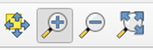
\includegraphics[width=0.95833in,height=\textheight]{images/clipboard-1487886273.png}
to zoom and out.

\textbf{Step 8:} Add the \textbf{P\_lakes.gpgk}. Right-click on this
layer in the layers panel and select \textbf{Attribute Table}. This
gives details about the polygon features of the dataset. The shape area
for each has been calculated in the `Shape\_Area' field.

\hypertarget{question-1}{%
\subsection*{Question 1:}\label{question-1}}
\addcontentsline{toc}{subsection}{Question 1:}

How many features (i.e.~shapes) are in the P\_lakes.gpkg?

\hypertarget{question-2}{%
\subsection*{Question 2:}\label{question-2}}
\addcontentsline{toc}{subsection}{Question 2:}

Where are the high versus low site indices relative to the terrain,
relative to the north versus south, and relative to roads?

\begin{center}\rule{0.5\linewidth}{0.5pt}\end{center}

\hypertarget{task-2-making-a-site-index-map}{%
\section*{Task 2: Making a Site Index
Map}\label{task-2-making-a-site-index-map}}
\addcontentsline{toc}{section}{Task 2: Making a Site Index Map}

\markright{Task 2: Making a Site Index Map}

\ul{Site index is a measure of productivity}. It is technically defined
as: \ul{\emph{expected height (m) of the best trees (not damaged,
biggest) of the dominant species at a reference age of 50 years breast
height age}}. The site index reflects the potential of the site to grow
this dominant species. Although this might also indicate how another
species might do, this does not give a measure of the possible
productivity of another species. For example, a site that is douglas-fir
leading and has a high site index would not indicate that a species like
whitebark pine (a high alpine species) would also do well. Also, if the
soils change (e.g., landslides, fertilization, etc.) or the
climate/hydrology changes, the site index might not be a good an
indicator of the productivity for the historically dominant species.
Importantly, for site index to be reported there have to be trees in the
stand. In the MKRF dataset some recently harvested stands may show a
``0'' for site index, but this is really an NA.

\textbf{Step 1} Load \textbf{P\_ForestCover\_1989.gpkg}. Right click on
the layer in the \textbf{layers} window and select \textbf{Open
Attribute Table}. this will open an attribute table that describes the
polygon components. Click on the the heading for \textbf{SITEINDX} to
sort the table from smallest to largest site index. Many polygons have
``0.0 m'' for a site index value. Scroll right to the ``non-forest
descriptor'' or \textbf{NFD} columbn. Here notes like ``NSR'' note sites
that are ``not-satisfactorily restocked, or there may be lakes. These
are examples of polygons where there are no trees and thus no site-index
value.

\textbf{Step 2} Click to the \textbf{SITEINDX} column heading again to
sort from largest to smallest. See \textbf{?@sec-Q3} to answer. Close
the attribute table.

\textbf{Step 3} Right click on the \textbf{P\_ForestCover\_1989} layer
again in the \textbf{layers} panel and select \textbf{Properties}

\begin{enumerate}
\def\labelenumi{\Alph{enumi}.}
\item
  Select \textbf{Symbology} and change the symbol from ``single Symbol''
  to ``Graduated''
\item
  Under \textbf{Value} click the small down arrow on the right to select
  the ``SITEINDX'' column.
\item
  In the \textbf{Color ramp} field click the small down arrow on the
  right to select the ``Viridis'' color palette
\item
  At the bottom of the symbology window, select \textbf{Classify}. This
  will classify the values in ``SITEINDX'' based on their values into
  different colors associated with the viridis color ramp.
\item
  Under \textbf{Classify} and \textbf{Mode} select ``Equal Interval''
  and change the number of \textbf{classes} to ``12''. Click
  \textbf{Classify} again.
\item
  In the \textbf{Classes} pain (the main white box) change these to
  \textbf{5 m classes} as 0.00 to 0.00 (i.e., no site index), 0.05 to
  5.05, 5.05 to 10.05, 10.05 to 15.05, etc.
\item
  Click \textbf{Apply and OK}. The symbology window will close and you
  can now see your recolored layer
\end{enumerate}

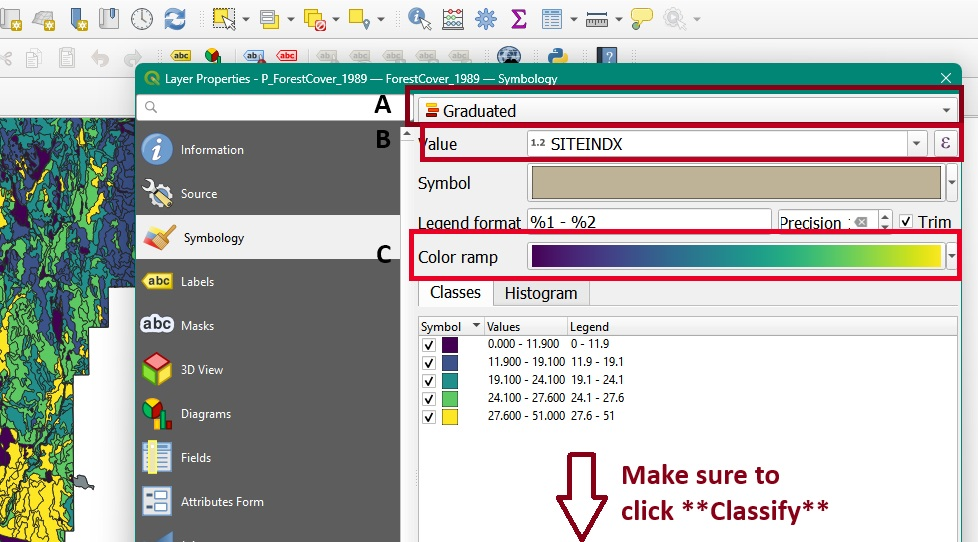
\includegraphics{images/QGIS image.jpg}

\textbf{Step 4} Create a site index map to export as a picture. :::
\{\#tip-mapmaking .callout-tip\} check out this link for some useful
resources on making maps in QGIS :::

\begin{enumerate}
\def\labelenumi{\Alph{enumi}.}
\item
  Select \textbf{Project} -\textgreater{} \textbf{New Print out}
  \textbf{Layout}. Name your print layout ``MRKF\_1989SiteIndex'' and
  click \textbf{OK.} A blank space appears in a new window with new
  Layout icons along the left-hand side.
\item
  In the left-hand of this new window, select
  
\includegraphics{images/clipboard-3366220892.png} to (\textbf{Add a
  New Map to the Layout)}. A \textbf{+} sign appears as a cursor. Drag
  the cursor around the blank area. Your map appears in this print
  layout. ~\textbf{NOTE:} If you do not see a map in \textbf{Layout
  View} use \textbf{Zoom Whole Page} =You may also need to reposition
  the map in the copied box using:
\end{enumerate}

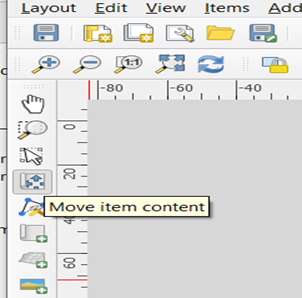
\includegraphics[width=2.57292in,height=3.13542in]{images/clipboard-3626068356.png}

\begin{enumerate}
\def\labelenumi{\Alph{enumi}.}
\setcounter{enumi}{2}
\item
  In the left-hand of this new window, select
  
\includegraphics{images/clipboard-3366220892.png} to (\textbf{Add a
  New Map to the Layout)}. A \textbf{+} sign appears as a cursor. Drag
  the cursor around the blank area. Your map appears in this print
  layout. ~\textbf{NOTE:} If you do not see a map in \textbf{Layout
  View} use \textbf{Zoom Whole Page} =You may also need to reposition
  the map in the copied box using:
\item
  \textbf{Right click} on your map and select \textbf{Page Properties}.
  Change the orientation from ``landscape'' to ``portrait''. ~
\item
  \textbf{Right click} on the map again and select \textbf{Item
  Properties} this time. Change the map scale (see the right-hand side
  of your screen for the properties) to expand your map to fill the
  page.~ A good scale value is 50000 which means 1 cm on the map
  represents 0.5 km (50,000 cm)
\item
  Use 
\includegraphics{images/clipboard-559090363.png} on the left-hand
  side to add a \textbf{Legend} (the + sign appears in the cursor, drag
  the cursor and Legend appears).
\item
  Use 
\includegraphics{images/clipboard-1747724821.png} to add a
  \textbf{Scale Bar.} Click on the \textbf{Item Properties} box. Change
  the ``Division Units'' to kilometres and then select a scale graphic
  you like.
\item
  Use 
\includegraphics{images/clipboard-769114577.png} to add a
  \textbf{Title}.
\item
  Add a north arrow by clicking
  
\includegraphics{images/clipboard-1756855161.png} and drag the curse
  to the map area.
\item
  Right click on each item on your map and select \textbf{Item
  Properties} to make any other changes to improve the appearance of
  your map. Alternatively, on the right-hand side there is \textbf{Item
  properties} icon where you can change the style of the items you added
  to the map (i.e., north arrow, legend, your map). NOTE: One could
  spend many hours on this! Just do some improvements.
\end{enumerate}

\textbf{Step 5} Export your map as an image. Go to \textbf{Layout} and
select \textbf{Export as Image.} Save the image the same location as
your document you are recording lab responses.

\hypertarget{question-3}{%
\subsection*{Question 3:}\label{question-3}}
\addcontentsline{toc}{subsection}{Question 3:}

What was the largest site index in m? What was the leading or dominant
species for that polygon? Give the full name and the Latin name for the
species.

\hypertarget{question-4}{%
\subsection*{Question 4:}\label{question-4}}
\addcontentsline{toc}{subsection}{Question 4:}

Add 5 m contours onto your map canvas. Where are the high versus low
site indices relative to the terrain, relative to the north versus
south, and relative to roads?

\hypertarget{map-1}{%
\subsection*{Map 1}\label{map-1}}
\addcontentsline{toc}{subsection}{Map 1}

Include your Site Index Map with a proper title, legend, scale, and
arrow bar.

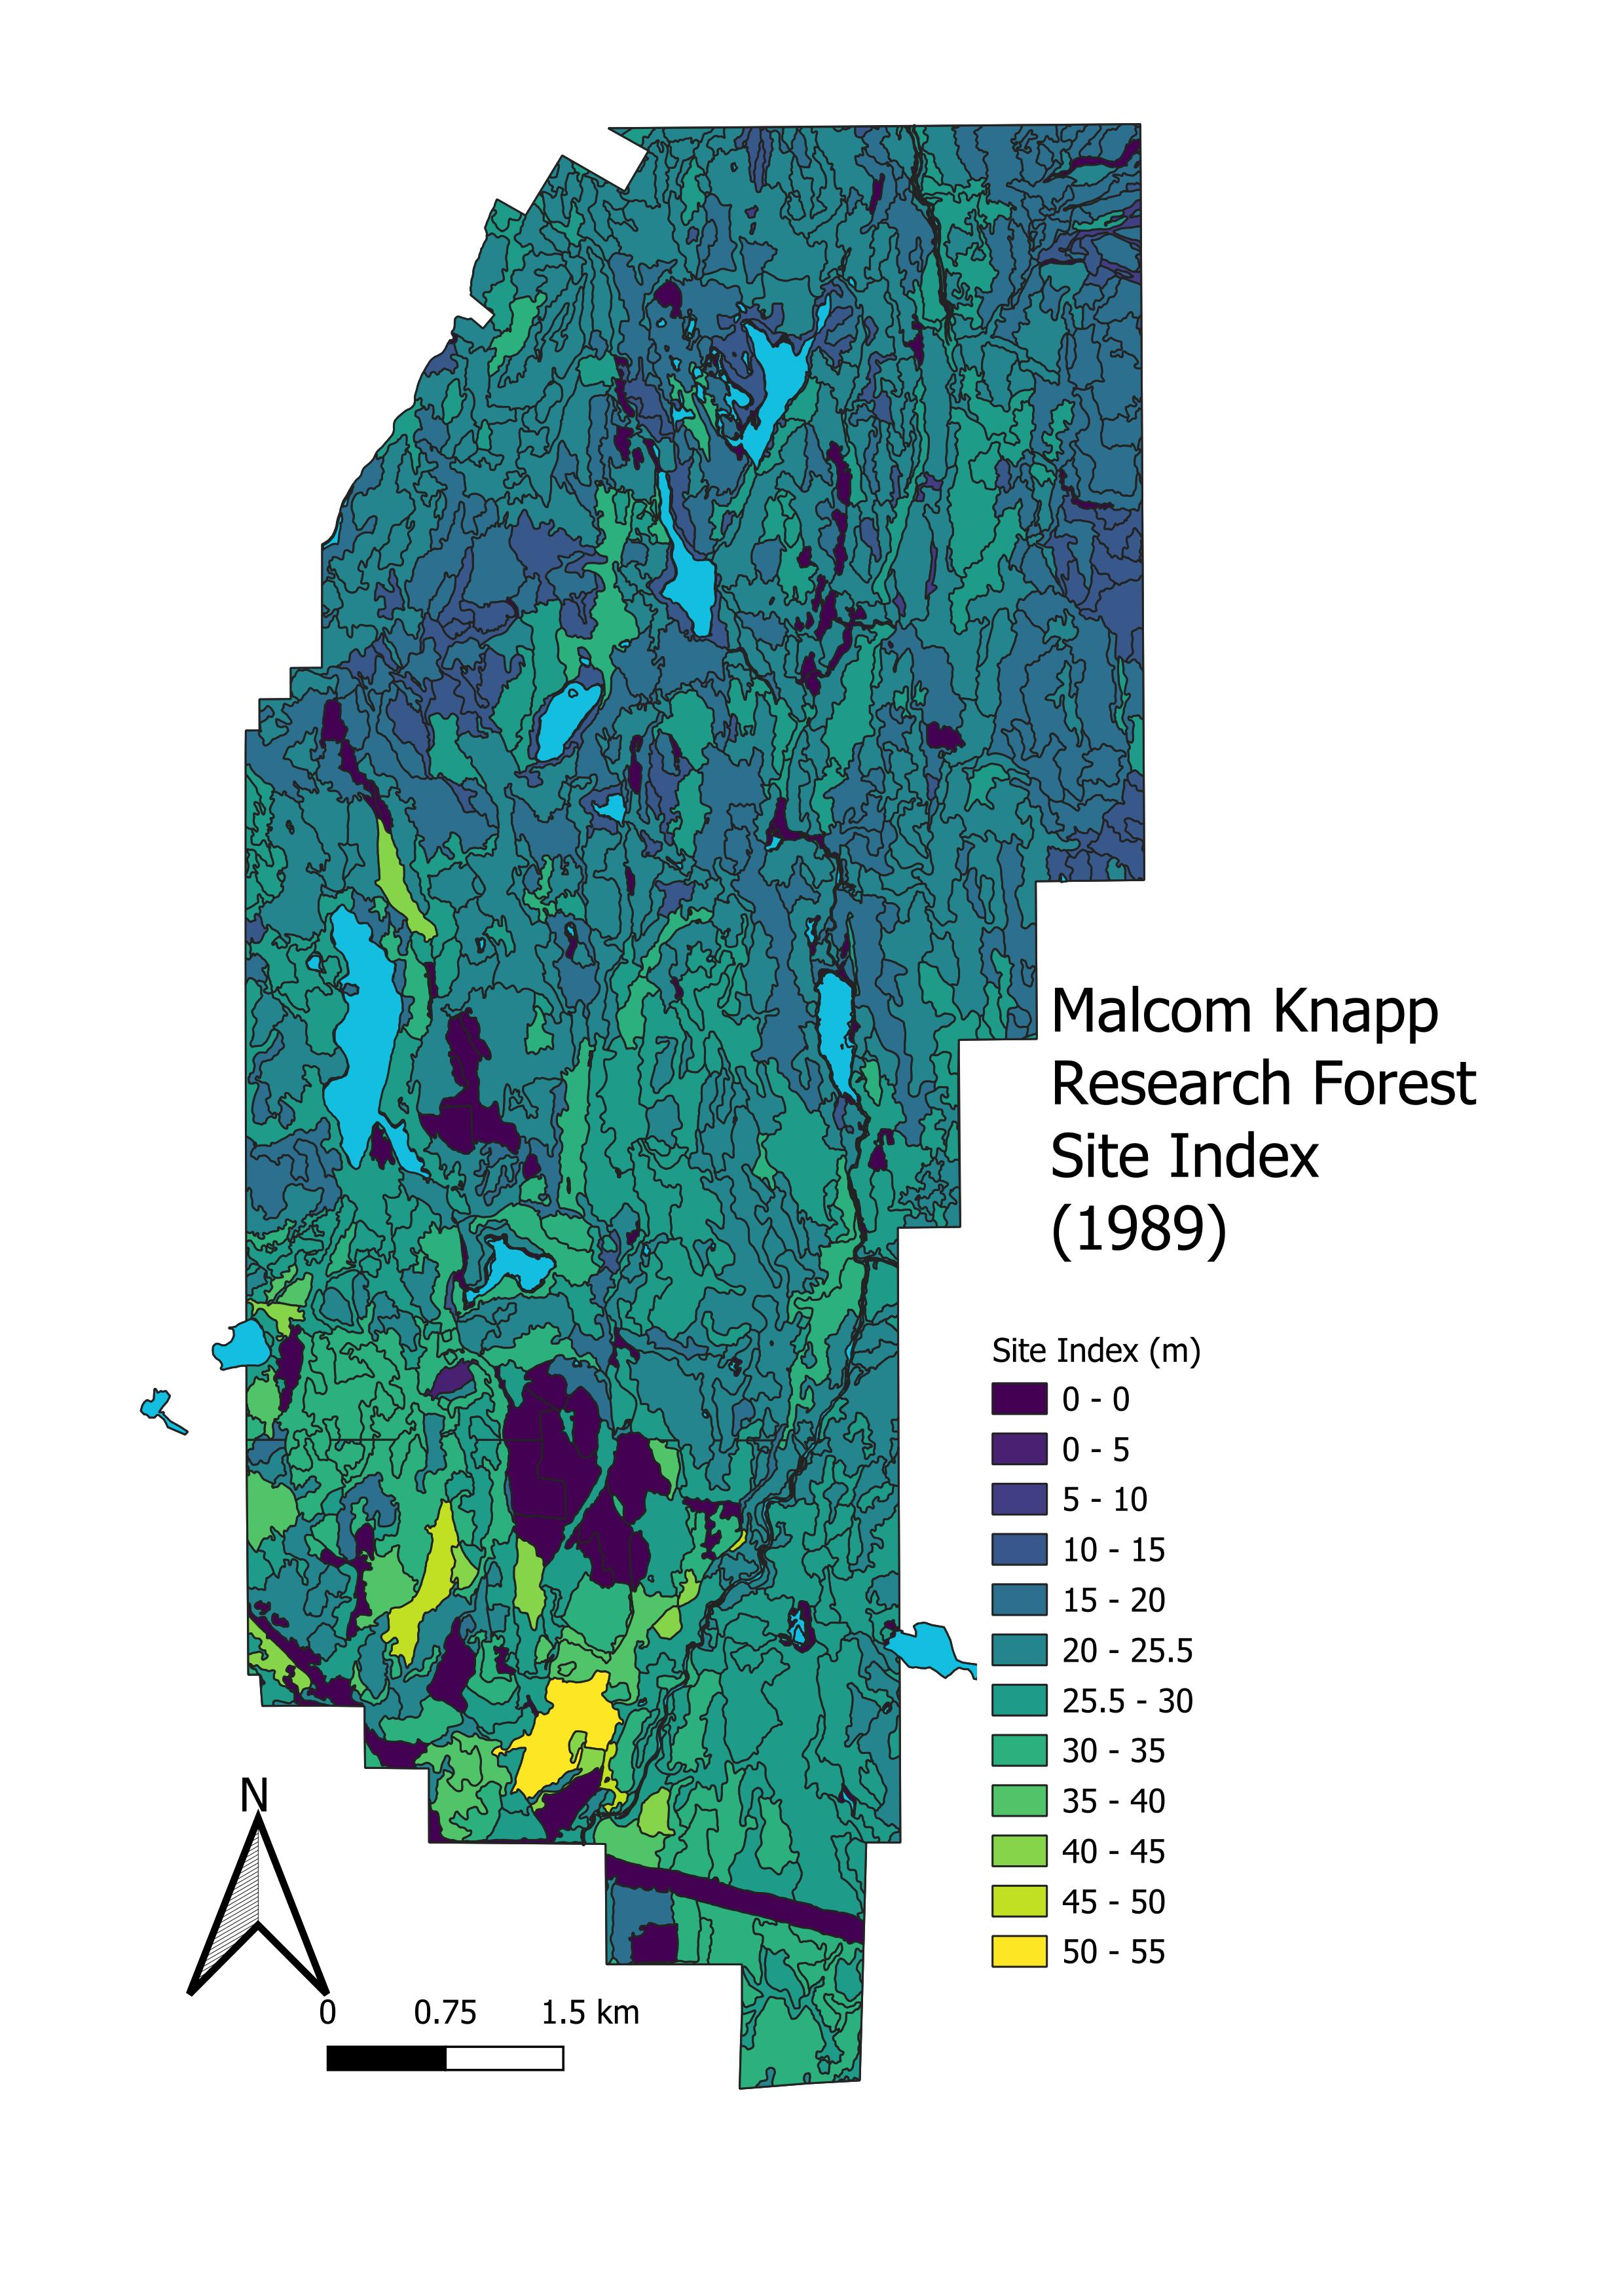
\includegraphics{images/Map1.jpg}

\begin{center}\rule{0.5\linewidth}{0.5pt}\end{center}

\hypertarget{task-3-visualize-stands-dominated-by-western-redcedar-in-1989}{%
\section*{Task 3: Visualize Stands Dominated by Western Redcedar in
1989}\label{task-3-visualize-stands-dominated-by-western-redcedar-in-1989}}
\addcontentsline{toc}{section}{Task 3: Visualize Stands Dominated by
Western Redcedar in 1989}

\markright{Task 3: Visualize Stands Dominated by Western Redcedar in
1989}

\textbf{Step 1} Close the \textbf{Layout} window and go back to the
\textbf{Data view} window again.

\textbf{Step 2} Change the \textbf{fc\_1989}-layer properties to a
\textbf{Single Symbol} again.

\textbf{Step 3} Right click on the \textbf{fc\_1989} layer and choose
\textbf{Open Attribute Table}. Each line of this table shows the
attributes for one polygon (including \textbf{SITEINDX} that you already
used). You can see the total number of polygons at the top of the
\textbf{Attribute Table} (1149 polygons). Keep this attribute table open
in this new window.

\textbf{Step 4} Select polygons where the first species is western
redcedar and the cedar is more than 50\% of the species composition. To
do so you will use a ``Query.'' To select \ul{polygons where the first
species is western redcedar and more than 50\% of the species
composition,} you will need to do a Query.

\begin{enumerate}
\def\labelenumi{\Alph{enumi}.}
\item
  In the \textbf{Attribute Table} select
  
\includegraphics{images/clipboard-3366763250.png} to open up the
  \textbf{Query Fields}
\item
  Scroll down a bit to find ``SPSC1'' and ``PCT1'', select for
  \textbf{SPSC1}=C and \textbf{PCT1}\textgreater=50. Click
  \textbf{Select Features}

  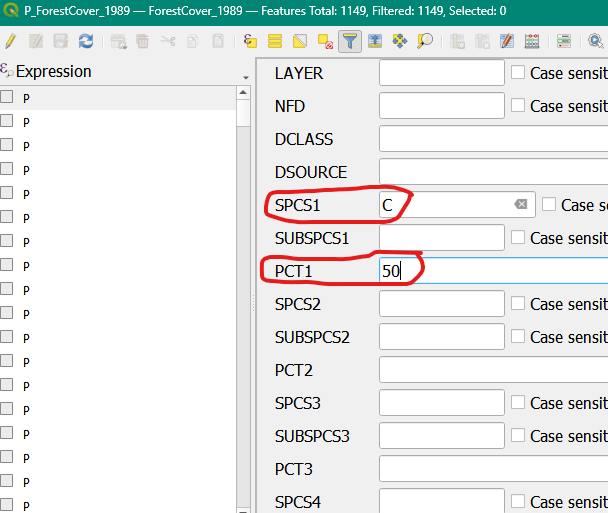
\includegraphics[width=3.75in,height=\textheight]{images/clipboard-1889425914.png}
\item
  Click the 
\includegraphics{images/clipboard-633541715.png} to return
  to the tabular format. You can see that we have now selected have a
  SPCS1 (leading species) of ``C'' for cedar, and that these polygons
  are \textgreater= 50\%. Use this to answer \textbf{question 5}
\end{enumerate}

\textbf{Step 6} Export your selection under it's own shapefile. You can
minimize or close the attribute table. In the \textbf{layers} panel
right click and select \textbf{Export -\textgreater{} Save Selected
Features As} save this as a gpkg file in the same folder as your MRKF
data. Name this \textbf{P\_FC\_1989\_CedarLeading.gpkg}.

\textbf{Step 7} Calculate the area and volume of cedar dominant stands
in 1989.

\begin{enumerate}
\def\labelenumi{\Alph{enumi}.}
\item
  Click on the \textbf{vector} icon in the top menu and go to
  \textbf{Analysis Tools -\textgreater{} Basic Statistics for Fields}
\item
  In the pop-up window select your P\_FC\_1989\_CedarLeading shapefile.
  In the \textbf{field to calculate statistics on} click the downward
  arrow and select ``Shape\_Area.'' Since this is a simple calculation,
  we will run this as a ``temporary output.'' Therefore, click
  \textbf{Run} on the bottom right.
\end{enumerate}

C. In the window that appears, find the \textbf{count, mean, and sum
values}. Use these to answer \textbf{?@sec-Q7} and question 8.

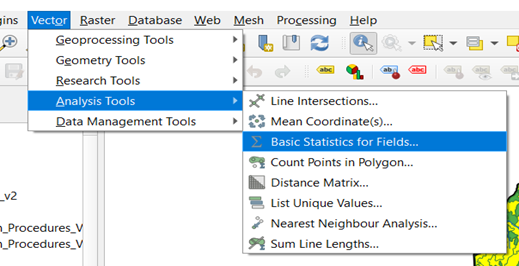
\includegraphics[width=4.83333in,height=\textheight]{images/clipboard-1197445832.png}

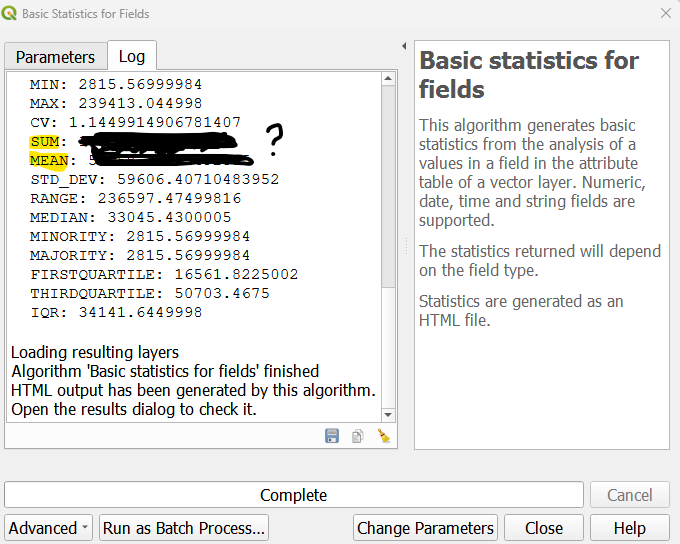
\includegraphics[width=3.5625in,height=\textheight]{images/clipboard-30022994.png}

\textbf{Step 9} Calculate the merchantable volume in the 1989 cedar
dominant stands.

\begin{enumerate}
\def\labelenumi{\Alph{enumi}.}
\item
  Right click on the P\_FC\_1989\_Cedarleading layer. Find the
  \textbf{Field Calculator}
  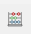
\includegraphics{images/clipboard-1506137763.png} tool.
\item
  In the pop-up window make sure \textbf{Create a new field} is checked.
  Input a formula to calculate shape area on. To calculate volume for
  the polygon, we need to use a measure of volume for the area. We have
  \textbf{VOL7\_5} which is the volume of trees per hectare that are
  \textgreater{} 7.5 cm. We also have \textbf{Shape\_Area} which is the
  area of the shape in m². We can use the following formula to calculate
  the volume per polygon

  \begin{equation}\protect\hypertarget{eq-volume}{}{Total~Volume (m³) = Polygon~Area (XX) * Volume (m³/ha)}\label{eq-volume}\end{equation}
\item
  Do a unit calculation to set up the equation. Shape\_area is in m² and
  VOL7\_5 is in m³/ha. If we want output to be in m³ what value do we
  need for XX ?
\item
  Name the field ``m3\_volume.'' Change the \textbf{Output field type}
  to ``Decimal number (real)'' and click \textbf{ok.} Estimates for
  volume for each polygon will now appear. Use these outputs to answer
  \textbf{?@sec-Q9}.
\item
  Use the \textbf{Calculate basic statistics tool} to calculate the
  average and total merchantable volumes in the cedar leading polygons.
\end{enumerate}

\textbf{Step 8} Make a map of the polygons dominated by western
redcedar. Look back towards @tip-mapmaking to remind yourself of the
process and the essential components to include in your map.

\hypertarget{question-5}{%
\subsection*{Question 5:}\label{question-5}}
\addcontentsline{toc}{subsection}{Question 5:}

\begin{enumerate}
\def\labelenumi{\Alph{enumi}.}
\tightlist
\item
  How many western redcedar (\textgreater= 50\%) polygons were there in
  1989?
\item
  Where are they located?
\item
  What polygons are not selected with the filter applied to the data?
\end{enumerate}

\hypertarget{question-6}{%
\subsection*{Question 6:}\label{question-6}}
\addcontentsline{toc}{subsection}{Question 6:}

What is the FULL latin name for western redcedar (including the namer -
a reference to the person that named the species)?

\hypertarget{sec-Q7}{%
\subsection*{Question 7:}\label{sec-Q7}}
\addcontentsline{toc}{subsection}{Question 7:}

What is the average polygon size (ha) for the western redcedar dominated
stands in 1989? NOTE: 10,000 m2=1 ha (i.e., 1 ha is 100m X 100 m =
10,000 m2)

\hypertarget{question-8}{%
\subsection*{Question 8:}\label{question-8}}
\addcontentsline{toc}{subsection}{Question 8:}

What is the total area in ha of all these selected polygons combined?

\hypertarget{question-9}{%
\subsection*{Question 9:}\label{question-9}}
\addcontentsline{toc}{subsection}{Question 9:}

What is the value of XX in Equation~\ref{eq-volume} above? Using this
equation, hat is the merchantable m3 volume (i.e., merchantable volume
for trees 7.50 DBH or larger) for all these selected polygons combined?
Do you feel like this a lot? (for reference a utility pole is
1m\^{}\^{}3)

\hypertarget{map-2}{%
\subsection*{Map 2:}\label{map-2}}
\addcontentsline{toc}{subsection}{Map 2:}

Include your map describing historically dominant cedar stands with a
proper title, legend, scale, and arrow bar.

\begin{center}\rule{0.5\linewidth}{0.5pt}\end{center}

\hypertarget{task-4-compare-changes-in-western-redcedar-from-1999-to-1989}{%
\section*{Task 4: Compare Changes in Western Redcedar from 1999 to
1989}\label{task-4-compare-changes-in-western-redcedar-from-1999-to-1989}}
\addcontentsline{toc}{section}{Task 4: Compare Changes in Western
Redcedar from 1999 to 1989}

\markright{Task 4: Compare Changes in Western Redcedar from 1999 to
1989}

Whew - you made it through the first interaction with QGIS in this
course. Congrats 🎉. Your instructors used the same steps that you used
for 989 to map and to get some statistics for western redcedar dominated
stands, but this time for 1999.~ There were 1,220 polygons in 1999 and
170 were dominated by western redcedar (Figure 1). The average polygon
size for these stands was 3.90 ha with a total number of ha of 662.53
ha. ~The merchantable volume for all of these stands combined was
319,903.0 m\textsuperscript{3}.

\hypertarget{question-10}{%
\subsection*{Question 10:}\label{question-10}}
\addcontentsline{toc}{subsection}{Question 10:}

Which year (1999 or 1989) had a large polygon size for western red-cedar
dominated stands? Please answer in hectares.

\hypertarget{question-11}{%
\subsection*{Question 11:}\label{question-11}}
\addcontentsline{toc}{subsection}{Question 11:}

Did the m3 for all these selected polygons combined increase or decrease
from 1989 to 1999?

\hypertarget{question-12}{%
\subsection*{Question 12:}\label{question-12}}
\addcontentsline{toc}{subsection}{Question 12:}

Based on your knowledge of forest dynamics so far, what might have
caused these differences area and volume of western redcedar dominated
stands between 1989 and 1999? HINT: Think about what human (e.g., new
roads, harvests, silvicultural treatments, etc.) and natural (e.g.,
fires, landslides, etc.) disturbances may have occurred for MKRF in the
CWH BEC zone in particular

\begin{center}\rule{0.5\linewidth}{0.5pt}\end{center}

\hypertarget{lab-questions-deliverables}{%
\section*{Lab Questions \&
Deliverables}\label{lab-questions-deliverables}}
\addcontentsline{toc}{section}{Lab Questions \& Deliverables}

\markright{Lab Questions \& Deliverables}

\begin{itemize}
\item[$\square$]
  Complete answers to the following questions:

  \begin{itemize}
  \tightlist
  \item[$\square$]
    Question 1: How many features (i.e.~shapes) are in the P\_lakes.gpkg
  \item[$\square$]
    Question 2: Where are the high versus low site indices relative to
    the terrain, relative to the north versus south and relative to
    roads?
  \item[$\square$]
    Question 3: What was the largest site index in m? What was the
    leading or dominant species for that polygon? Give the full name and
    the Latin name for the species.
  \item[$\square$]
    Question 4: Where are the high versus low site indices relative to
    the terrain, relative to the north versus south, and relative to
    roads?
  \item[$\square$]
    Question 5: (a) How many western redcedar (\textgreater= 50\%)
    polygons were there in 1989? (b) Where are they located? (c) What
    polygons are not selected with the filter applied to the data?
  \item[$\square$]
    Question 6: What is the FULL latin name for western redcedar
    (including the namer - a reference to the person that named the
    species)?
  \item[$\square$]
    Question 7: What is the average polygon size (ha) for the western
    redcedar dominated stands in 1989? NOTE: 10,000 m2=1 ha (i.e., 1 ha
    is 100m X 100 m = 10,000 m2)
  \item[$\square$]
    Question 8: What is the total area in ha of all these selected
    polygons combined?
  \item[$\square$]
    Question 9: What is the merchantable m3 volume (i.e., merchantable
    volume for trees 7.50 DBH or larger) for all these selected polygons
    combined? Do you feel like this a lot? (for reference a utility pole
    is 1m\^{}\^{}3)
  \item[$\square$]
    Question 10: Which year (1999 or 1989) had a large polygon size for
    western red-cedar dominated stands? Please answer in hectares.
  \item[$\square$]
    Question 11: Did the m3 for all these selected polygons combined
    increase or decrease from 1989 to 1999
  \item[$\square$]
    Question 12. Based on your knowledge of forest dynamics so far, what
    might have caused these differences area and volume of western
    redcedar dominated stands between 1989 and 1999? HINT: Think about
    what human (e.g., new roads, harvests, silvicultural treatments,
    etc.) and natural (e.g., fires, landslides, etc.) disturbances may
    have occurred for MKRF in the CWH BEC zone in particular
  \end{itemize}
\item[$\square$]
  Complete Maps for :

  \begin{itemize}
  \tightlist
  \item[$\square$]
    A site index map for Malcom Knapp Research Forest
  \item[$\square$]
    A map showing the locations of the Western Red Cedar leading forest
    polygons from 1989.
  \item
    Make sure that your map includes:

    \begin{itemize}
    \tightlist
    \item
      A title
    \item
      A scale bar
    \item
      A north arrow
    \item
      A proper legend
    \end{itemize}
  \end{itemize}
\end{itemize}

\hypertarget{summary}{%
\section*{Summary}\label{summary}}
\addcontentsline{toc}{section}{Summary}

\markright{Summary}

\bookmarksetup{startatroot}

\hypertarget{terrain-spatial-interpolation}{%
\chapter{Exercise 2: VRI Forest Cover and Digital
Imagery}\label{terrain-spatial-interpolation}}

Written by

Sarah Smith-Tripp

\hypertarget{lab-overview-1}{%
\section*{Lab Overview}\label{lab-overview-1}}
\addcontentsline{toc}{section}{Lab Overview}

\markright{Lab Overview}

British Columbia relies heavily on surveying from aerial imagery to
understand forest health. Aerial surveys have been used throughout BC's
recent history to understand forest composition and health. Aerial
imagery is the key input into the vegetation resource inventory (or VRI)
used to understand the composition of BCs forests. The process has two
phases:

\begin{itemize}
\item
  Phase 1: Using aerial imagery, forests are divided into homogeneous
  areas called ``polygons.''
\item
  Phase 2: Ground-reference plots are placed systematically throughout
  polygons. Ground-reference plots are used to determine the site-type
  or biogeoclimatic zone and subzone of each area. You can find more
  information on this process
  \href{https://cfcg.forestry.ubc.ca/resources/cataloguing-in-situ-genetic-resources/about-bec-and-bgc-units/}{here}.
\end{itemize}

These data are collectively used to obtain information on the forests of
BC.~However, since forests change over time, VRI also includes
\ul{regular updates} of original VRI data to reflect changes in forest
composition associated with:

\begin{itemize}
\item
  \ul{Large-scale} \ul{natural disturbances}:~e.g., fires, insects,
  windthrow, etc.
\item
  \ul{Human disturbances}:~e.g., clear-cuts, partial harvests, roads,
  new urban areas, etc.
\end{itemize}

These new openings result in \ul{changes to polygon boundaries and
attributes relative to prior dates for the same land area}.~ In
addition, \ul{the attributes of each forested polygon are forecasted for
stand-level growth to the current date (labelled as ``Projected'')}.~
For example, if the stand age was 50 years in 2000, the updated age
(called ``Projected Age'') in 2015 is 50+15=65 years. There are some
attributes such as species composition that cannot be accurately updated
via a forecast.~ \ul{At some point, a re-inventory is needed}.
Typically, the Province does not regularly update the VRI layers for
disturbances on private lands. The VRI for MKRF was actually updated to
an entirely new reference year in 2020. We've included this data with
the course and will introduce it at the end of lab. You can see that the
2014 VRI is largely the same as the 1996 VRI, but when the VRI was
updated to a new reference year there were many changes.

\begin{center}\rule{0.5\linewidth}{0.5pt}\end{center}

\hypertarget{learning-objectives-1}{%
\section*{Learning Objectives}\label{learning-objectives-1}}
\addcontentsline{toc}{section}{Learning Objectives}

\markright{Learning Objectives}

\begin{itemize}
\item
  Examine differences in the 2014 VRI compared to forest cover layers
\item
  Complete an initial photo-interpretation for forest cover maps using
  the 2014 VRI standards. Your approach will use a 2D image, but
  photointerpreters normally use images ``stereo-imagery'' which
  combines images to create a 3D representation of the imagery.
\item
  Compare the aerial images to images from Landsat satellites and
  consider how these might be useful for updated forest land changes.
\end{itemize}

\begin{center}\rule{0.5\linewidth}{0.5pt}\end{center}

\hypertarget{task-1-discover-the-difference-between-forest-cover-and-vri}{%
\section*{Task 1: Discover the difference between ``Forest Cover'' and
VRI}\label{task-1-discover-the-difference-between-forest-cover-and-vri}}
\addcontentsline{toc}{section}{Task 1: Discover the difference between
``Forest Cover'' and VRI}

\markright{Task 1: Discover the difference between ``Forest Cover'' and
VRI}

Last week, we used forest cover polygons to look at the forest cover
from 1989 and briefly compared changes between 1989 and 1999. These
forest cover polygons were created using interpretation of aerial
imagery. Both VRI and forest cover polygons intrept components of
forests using aerial imagery. However, their standards for
photo-interpretation are different.

In our dataset, the forest cover polygons are based on
photointepretation of 1987 photos, while the 2014 VRI is based on a
19996 aerial survey. Forest cover polygons are updated for natural and
human disturbances, whereas VRI polygons are updated for the same
disturbances. VRI polygons are also projected to the updated year.
Additionally, VRI includes information on four different forest
structure layers, from top canopy to the shrub layer. In this lab, we
will work with the top of canopy layer. You can find out more on what
attributes are recorded in
\href{https://www2.gov.bc.ca/assets/gov/farming-natural-resources-and-industry/forestry/stewardship/forest-analysis-inventory/data-management/standards/vegcomp_poly_rank1_data_dictionaryv5_2019.pdf}{the
VRI data dictionary.}

\hypertarget{building-familiarity-with-vri-data}{%
\subsubsection*{Building Familiarity with VRI
data}\label{building-familiarity-with-vri-data}}
\addcontentsline{toc}{subsubsection}{Building Familiarity with VRI data}

\textbf{Step 1:} Open QGIS and save a new map project. Set up this
project similarly to how we did in Task 1 lab 1 (INCLUDE REFERENCE
HERE).

\textbf{Step 2:} Add the following layers to your blank map:

\begin{itemize}
\tightlist
\item
  P\_Boundary\_MRKF
\item
  P\_BC\_VRI\_2014
\item
  P\_ForestCover\_1989
\end{itemize}

\textbf{Step 3:} Select ``P\_BC\_VRI\_2014'' and change the layer
symbology. Change the outline to ``white'' ⬜change the fill color to
``light grey'' and increase the outline stroke width 0.2 mm. Click
\textbf{Apply and Ok.}

\textbf{Step 4:} Select the ``P\_ForestCover\_1989'' and change the
symbology. Change the outline color to ``orange🟧''

\textbf{Step 5:} Compare the VRI polygons to the 2006 Orthomosaic. Are
there areas where the VRI projection does not make sense? To answer
this, set the fill color for the VRI to semi-translucent and zoom to:
1250396, 481902 (*\emph{make sure your map CRS is set to BC Conus
Albers; EPSG 3005)}. You can paste these values into the coordinate box
on the bottom of the screen.


\includegraphics[width=2.39583in,height=0.26042in]{images/clipboard-2547981647.png}

\textbf{Step 6:} Load in P\_ForestCover\_2008. This is the updated
forest cover layer as of 2006. Find the name of the forest disturbance
that occurred in 2006 at the location identified in \textbf{step 5}

\hypertarget{question-1-1}{%
\subsection{Question 1:}\label{question-1-1}}

Which description of forest composition and structure (VRI and forest
cover) has more polygons?

\hypertarget{question-2-1}{%
\subsection{Question 2:}\label{question-2-1}}

Which descriptor of forest composition has a larger average polygon?
Which one has a larger maximum polygon?

\hypertarget{question-3-1}{%
\subsection{Question 3:}\label{question-3-1}}

What is the projected age for the polygon at this site? Does this make
sense? Why or why not? Insert a screenshot (include a figure caption!)
to support your answer.

\hypertarget{question-4-1}{%
\subsection{Question 4:}\label{question-4-1}}

Look for two other forest disturbances or land-cover changes anywhere in
MKRF recorded in the 2006 orthomosaic but not recorded in the 2014 VRI.

\hypertarget{question-5-1}{%
\subsection{Question 5:}\label{question-5-1}}

Malcom Knapp is privately owned land, meaning not all disturbances are
consistently added to VRI. Given this, what are some of the
disadvantages of relying on VRI alone? What additional tools can we use
to better update VRI? Respond in a clear and well written paragraph
format.

\begin{center}\rule{0.5\linewidth}{0.5pt}\end{center}

\hypertarget{task-2-segmenting-forest-polygons}{%
\section*{Task 2: Segmenting Forest
Polygons}\label{task-2-segmenting-forest-polygons}}
\addcontentsline{toc}{section}{Task 2: Segmenting Forest Polygons}

\markright{Task 2: Segmenting Forest Polygons}

Read through the
\href{https://www2.gov.bc.ca/assets/gov/farming-natural-resources-and-industry/forestry/stewardship/forest-analysis-inventory/forest-cover-inventories/photo-interpretation/standards/vri_photo_interpretation_procedures_version_39.pdf\#page=21.84}{photo-interpretation
standards} provided by the Ministry. Note that the linked version is
version 5 - reflecting that these standards are fifth version of VRI
photo-interpretation standards since 1999 (when the VRI program was
established). Focus on \textbf{Figure 2.1 and Figure 2.2}. These show
initial steps in segmenting the land base into forest cover polygons.
You will be interpreting a 2006 photo of area of MKRF using these two
figures and ``heads-up digitizing.'' Normally, this first step would be
done using a 3-D view of overlapping aerial images. You will be using a
2-D view for this first step in photo-interpretation to get an idea of
how this is initially done. These larger polygons would be further
stratified using forest cover attributes, and all attributes added as
documented in the VRI photo-interpretation standards.

\textbf{Step 1} Add the 2008 and the 2006 aerial imagery to your map.
Note that the 2008 photo is only part of the MRKF

\textbf{Step 2} zoom into the three following locations below. Create a
\emph{formatted} table to answer question 6 (@sec-Q6)

\textbf{Step 3} zoom into a clearcut location in 2008. Think about what
characteristics support it is harvested

\hypertarget{sec-Q6}{%
\subsection*{Question 6:}\label{sec-Q6}}
\addcontentsline{toc}{subsection}{Question 6:}

Zoom into the locations noted on the table. Use the
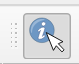
\includegraphics[width=0.28125in,height=\textheight]{images/clipboard-1450729439.png}
tool located in the upper right of QGIS to retrieve RGB values for the
following areas. Once you have filled in the table, discuss why you
think different landcovers have different pixel values.

\begin{tcolorbox}[enhanced jigsaw, colbacktitle=quarto-callout-note-color!10!white, leftrule=.75mm, left=2mm, opacitybacktitle=0.6, breakable, colframe=quarto-callout-note-color-frame, arc=.35mm, bottomtitle=1mm, rightrule=.15mm, title=\textcolor{quarto-callout-note-color}{\faInfo}\hspace{0.5em}{Note}, toptitle=1mm, titlerule=0mm, opacityback=0, coltitle=black, colback=white, bottomrule=.15mm, toprule=.15mm]

NOTE: Remember that for a color rendition of an image, white objects
reflect high in all visual bands; green objects reflect higher in the
green band; blue objects reflect higher in the blue band; red objects
reflect higher in the red band; and black objects have low reflectance
in all visual bands.

\end{tcolorbox}

\begin{longtable}[]{@{}
  >{\raggedright\arraybackslash}p{(\columnwidth - 10\tabcolsep) * \real{0.1139}}
  >{\raggedright\arraybackslash}p{(\columnwidth - 10\tabcolsep) * \real{0.1013}}
  >{\raggedright\arraybackslash}p{(\columnwidth - 10\tabcolsep) * \real{0.1392}}
  >{\raggedright\arraybackslash}p{(\columnwidth - 10\tabcolsep) * \real{0.2025}}
  >{\raggedright\arraybackslash}p{(\columnwidth - 10\tabcolsep) * \real{0.2278}}
  >{\raggedright\arraybackslash}p{(\columnwidth - 10\tabcolsep) * \real{0.2152}}@{}}
\caption{Pixel brightness values for different land cover types in
MKRF}\tabularnewline
\toprule\noalign{}
\begin{minipage}[b]{\linewidth}\raggedright
E
\end{minipage} & \begin{minipage}[b]{\linewidth}\raggedright
N
\end{minipage} & \begin{minipage}[b]{\linewidth}\raggedright
Landcover
\end{minipage} & \begin{minipage}[b]{\linewidth}\raggedright
Red Brightness
\end{minipage} & \begin{minipage}[b]{\linewidth}\raggedright
Green Brightness
\end{minipage} & \begin{minipage}[b]{\linewidth}\raggedright
Blue Brightness
\end{minipage} \\
\midrule\noalign{}
\endfirsthead
\toprule\noalign{}
\begin{minipage}[b]{\linewidth}\raggedright
E
\end{minipage} & \begin{minipage}[b]{\linewidth}\raggedright
N
\end{minipage} & \begin{minipage}[b]{\linewidth}\raggedright
Landcover
\end{minipage} & \begin{minipage}[b]{\linewidth}\raggedright
Red Brightness
\end{minipage} & \begin{minipage}[b]{\linewidth}\raggedright
Green Brightness
\end{minipage} & \begin{minipage}[b]{\linewidth}\raggedright
Blue Brightness
\end{minipage} \\
\midrule\noalign{}
\endhead
\bottomrule\noalign{}
\endlastfoot
1248400 & 481890 & & & & \\
1247760 & 848198 & & & & \\
1248195 & 483318 & & & & \\
1247019 & 483138 & & & & \\
\end{longtable}

\hypertarget{question-7}{%
\subsection*{Question 7:}\label{question-7}}
\addcontentsline{toc}{subsection}{Question 7:}

When you look at a clear cut area, what characteristics support an area
is harvested? Consider size, shape, texture, proximity to other
features, etc. List three specific characteristics to identify a
harvested area that you could give to someone else who has never seen an
above view of a clear cut.

\hypertarget{question-8-1}{%
\subsection*{Question 8:}\label{question-8-1}}
\addcontentsline{toc}{subsection}{Question 8:}

Create a reference table that describes specific characteristics that
can help differentiate land cover types using aerial imagery. For each
feature in the below table include 3 characteristics of the different
land covers.

\begin{longtable}[]{@{}ll@{}}
\toprule\noalign{}
Land cover type & Key Characteristics \\
\midrule\noalign{}
\endhead
\bottomrule\noalign{}
\endlastfoot
Road & \\
Partially Harvested Stand & \\
Hydro Electrical clearing & \\
\end{longtable}

\hypertarget{task-3-understand-variability-in-pixel-data}{%
\section*{Task 3: Understand Variability in Pixel
Data}\label{task-3-understand-variability-in-pixel-data}}
\addcontentsline{toc}{section}{Task 3: Understand Variability in Pixel
Data}

\markright{Task 3: Understand Variability in Pixel Data}

We have established an understanding of the key characteristics of
different land cover types and how these relate to brightness values. We
will now use QGIS to create a new polygon feature that will help better
understand variability in pixel data, and how this variability can help
us explore our datasets.

\textbf{Step 1} Create a new shapefile layer by going to \textbf{Layer
-\textgreater{} Create a Layer -\textgreater{} Create a new shapefile
layer}

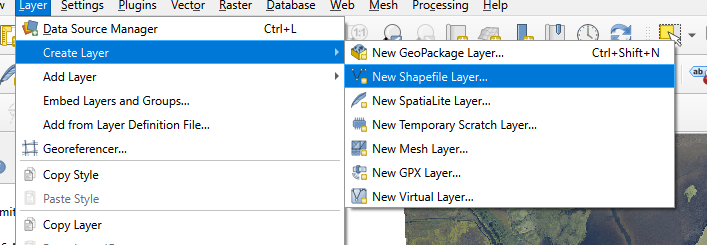
\includegraphics{images/clipboard-477174409.png}

\textbf{Step 2} Save your shapefile to the same location as your
exercise two, name this layer ``Landcover Types.shp''. For the
\textbf{Geometry Type} select ``polygon.'' In the \textbf{New Field}
window create a \textbf{Text} field called ``class.'' Make sure to click
\textbf{Add to Fields List.} Click \textbf{Ok.} Your new layer should
appear in the layers panel.

\textbf{Step 3} Right click on your new layer in the \textbf{layers
panel.} Select \textbf{Toggle Editing.} The layer can now be actively
edited.

\textbf{Step 4} Click on the polygon tool
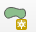
\includegraphics{images/clipboard-3885190170.png} in the upper left of
the screen. This tool allows you to add new polygons to your shapefile.
To add a polygon, left-click to begin a shape and add addition vertices.
To finish a shape \textbf{right-click.} Use this process to add polygons
that cover (a) a fresh clearcut (b) a lake (c) an older clearcut (d) a
mixed forest (e) coniferous forest in the \ul{\textbf{2006}} \textbf{RGB
image}. When you finish a polygon make sure to note the landcover type
in your ``class'' field.

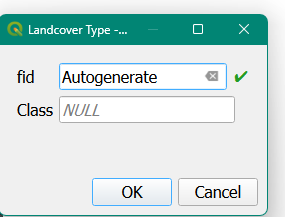
\includegraphics[width=2.46875in,height=\textheight]{images/clipboard-1460819033.png}

\textbf{Step 5} once you have finished right-click on your layer in the
\textbf{Layers} panel to save the layer edits. Additionally, change the
\textbf{symbology} of this layer to show the individual layer
attributes. See an example in Figure~\ref{fig-1}.

\begin{figure}

{\centering 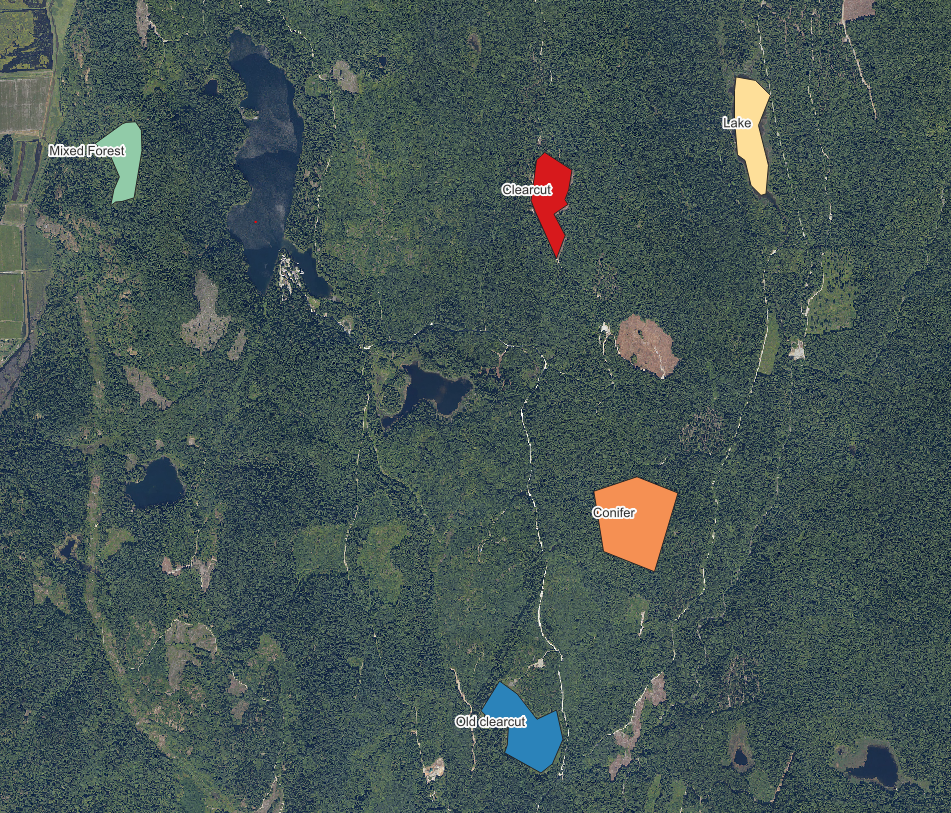
\includegraphics[width=5.75in,height=\textheight]{images/clipboard-1582844239.png}

}

\caption{\label{fig-1}Landcover types for polygon based on
interpretation of 2006 aerial RGB imagery. \emph{Note that 2008 is shown
in background}}

\end{figure}

\textbf{Step 5} We will now introduce the \textbf{processing toolbox}.
This is a great resource for finding tools that help analyze spatial
data. The processing toolbox is normally located on the upper right-hand
of of the QGIS window. If it is not there, you can load it by going to
\textbf{View -\textgreater{} Panels -\textgreater{} Processing Toolbox.}

\begin{figure}

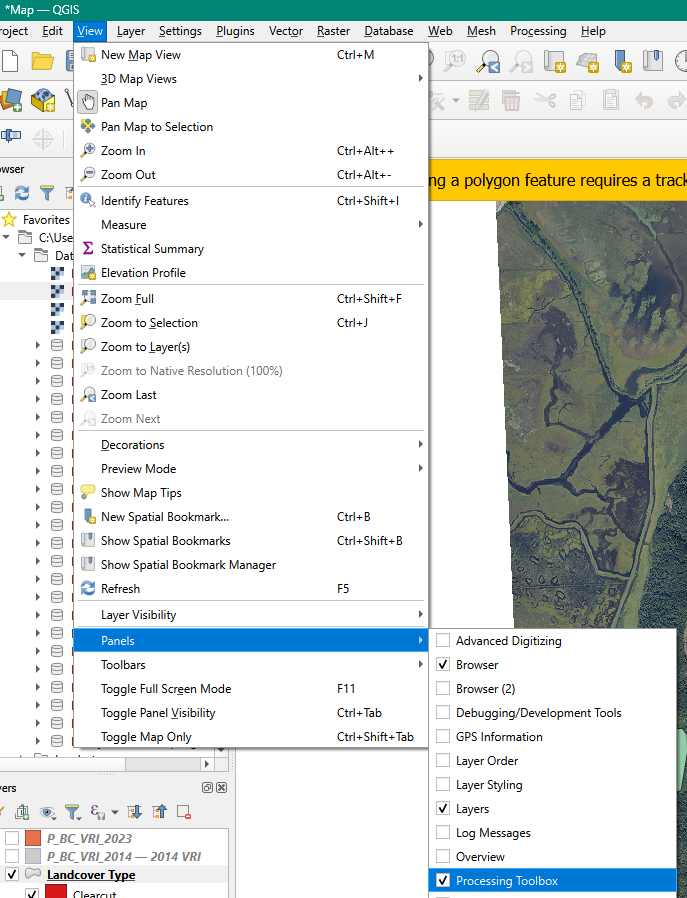
\includegraphics[width=4.89583in,height=\textheight]{images/clipboard-3381024759.png} \hfill{}

\end{figure}

\textbf{Step 6} In the search bar located at the top of the
\textbf{processing toolbox} type in ``Zonal'' and select \textbf{Zonal
statistics.} In the pop-up window make the following selections

\begin{enumerate}
\def\labelenumi{\Alph{enumi}.}
\tightlist
\item
  \textbf{Input layer:} Select your class polygons
\item
  \textbf{Raster layer}: Select the \textbf{2006 RGB} image
\item
  \textbf{Raster band:} Select the green band
\item
  \textbf{Output column prefix:} type ``\emph{Brt'' (for pixel
  brightness values})
\item
  \textbf{Right click on the ``\ldots{}'' in statistics to calculate.}
  In the new menu select (1) Mean (2) St Dec (2) Minimum and (3) maximum
\item
  \textbf{Save the file to the same location as your exercise 2}
\end{enumerate}

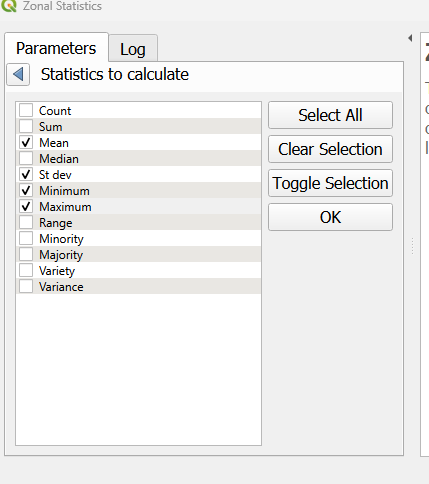
\includegraphics[width=4.17708in,height=\textheight]{images/clipboard-1244300705.png}

\textbf{Step 7} Using the new shapefile, color the shapefile by mean
brightness. Under \textbf{symbology} select ``graduated'' and for the
color palette choose ``greys.'' At the top to the color palette window
choose \textbf{invert color ramp}. Inverting the color ramp means that
the polygons where the mean brightness values is low will be closer to
black and polygons where the mean brightness is high will be closer to
white.

\textbf{Step 8} We will now create a new map layout to showcase some the
forest cover polygons we have created. Go to file \textbf{New print
layout} andcreate a new map layout named ``forest cover polygons.'' Make
the orientation of new map \textbf{horizontal.} Our new map layout will
have three different maps. The first, will describe the forest cover
polygons we have created. The second, will describe in the mean
brightness for the RGB data we have. Finally, we will have a third map
that will look at the variability in these brightness responses.

\textbf{Step 9} We'll start with the map the describes our forest
polygons.

\begin{enumerate}
\def\labelenumi{\Alph{enumi}.}
\tightlist
\item
  change the symbology of the forest polygons shapefile to give each
  polygon a unique color. Go to symbology -\textgreater{} categorized
  -\textgreater{} select your ``class'' field -\textgreater{} and
  classify. Click \textbf{Apply} but NOT \textbf{ok.}
\item
  On the left-hand of this pop-up window go to ``labels'' and select
  \textbf{Single Label} for \textbf{Value} select your ``class'' field.
\item
  Click on \textbf{Buffer} and check the box that says \textbf{Draw text
  Buffer} this will put a small white buffer around our labels
\item
  Click on \textbf{Placement} change the \textbf{mode} to \textbf{Offset
  from centroid}. Click the box that says \textbf{Allow placing of
  labels outside of polygons.} Change the \textbf{Quadrant} to the
  upper-left
\item
  Click \textbf{Apply} - labels should now appear on the map canvas
\item
  Click \textbf{Ok.}
\end{enumerate}

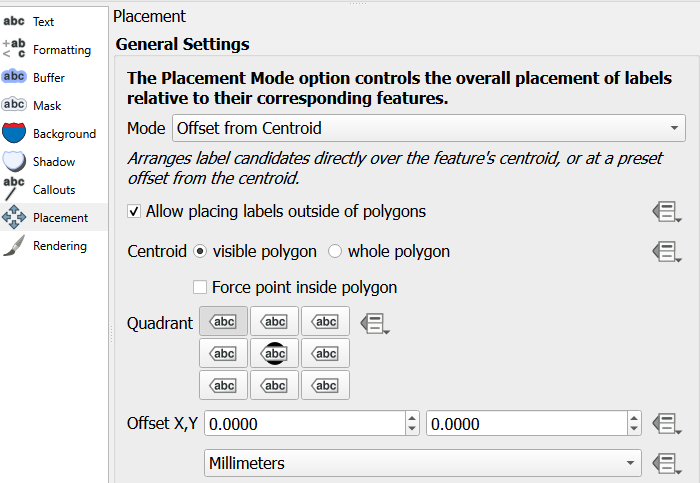
\includegraphics{images/clipboard-74741472.png}

\begin{enumerate}
\def\labelenumi{\Alph{enumi}.}
\setcounter{enumi}{6}
\tightlist
\item
  Navigate back to your map layout. Insert a new map for your forest
  polygons. In the background, include the BC VRI and 2008 RGB image.
  The screenshot below highlights what should be included. Set the map
  scale to 70000 to best include all of MKRF.
\end{enumerate}

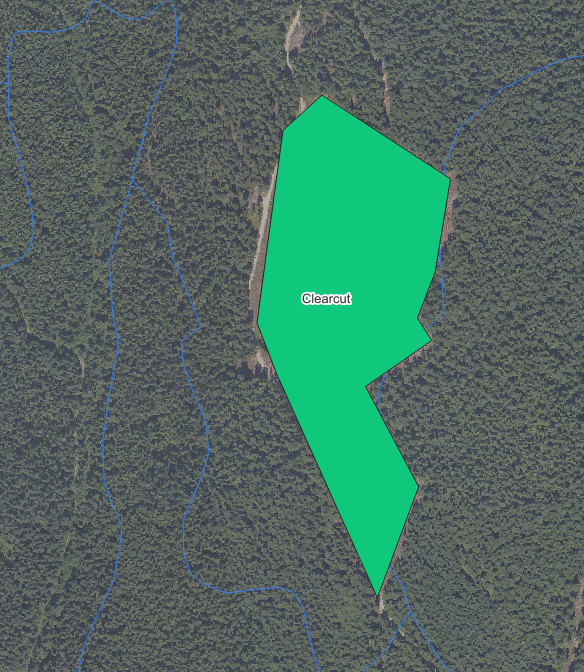
\includegraphics[width=3.60417in,height=\textheight]{images/clipboard-1857806976.png}

\begin{enumerate}
\def\labelenumi{\Alph{enumi}.}
\setcounter{enumi}{7}
\item
  In the right-hand side under \textbf{Layers} click the checkmark that
  says \textbf{Lock layers and Lock styles for Layers} this prevents
  your map from automatically updating.
\item
  Add a legend\textbf{.} In \textbf{Legend items} uncheck ``auto
  update'' and remove all legend items are are not your forest cover
  polygons. On the forest polygon layer right-click to check ``hidden.''
  In the \textbf{Title} for the legend put ``Forest Polygon Class''
\item
  Right click on the map on your map layout to \textbf{copy and paste}
  the map so there is a duplicate map next to your forest polygon map.
  With this map selected \textbf{uncheck} the \textbf{Lock layers and
  Lock styles for Layers}. Navigate back to your map canvas
\end{enumerate}

\textbf{Step 9} We'll now map the average green brightness value in
these polygons.

\begin{enumerate}
\def\labelenumi{\Alph{enumi}.}
\tightlist
\item
  Using your layer that we calculated zonal statistics on, which should
  still be colored black-to-white. Move this layer to the top of the map
  canvas.
\item
  Navigate back to your map layout. With the copied map selected change
  the name to ``zonal mean.'' In the item properties tab click the
  circular ``refresh'' button. This will update the map to the current
  canvas layers. Click \textbf{Lock layers and Lock styles for Layer.}\\
  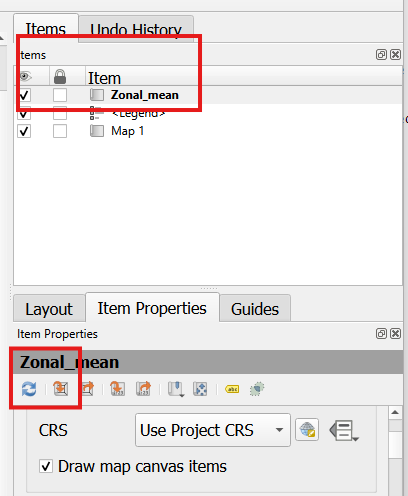
\includegraphics{images/clipboard-1003007197.png}
\item
  Copy the Legend from your polygons layer. Change the reference map to
  the zonal statistics layer. In the legend properties check ``update
  all''. Change the \textbf{Title} to ``Mean Bit Brightness (Green
  Band)''.\\
  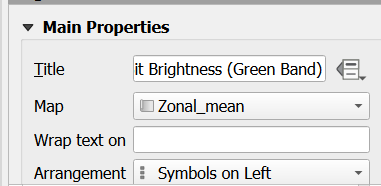
\includegraphics{images/clipboard-798660786.png}
\item
  Right click on the map on your map layout to \textbf{copy and paste}
  the map so there is a duplicate map next to your forest zonal
  statistics map. With this map selected \textbf{uncheck} the
  \textbf{Lock layers and Lock styles for Layers}. Navigate back to your
  map canvas.
\end{enumerate}

\textbf{Step 10} Follow a similar process to step 9, but this time
change the zonal statistics layer to the standard deviation. See
Figure~\ref{fig-2} for an example of your final output.

\begin{figure}

{\centering \includegraphics{images/ForestCoverMap.png}

}

\caption{\label{fig-2}Example output for forest cover map. **Note your
map will be different according to where you place your polygons}

\end{figure}

\hypertarget{question-9-1}{%
\subsection*{Question 9:}\label{question-9-1}}
\addcontentsline{toc}{subsection}{Question 9:}

How do values for your different forest polygons layer differ in terms
of brightness? What feature had the highest greenness reflectance? Which
feature had the most variable greenness reflectance? Use values to
support your results.

\hypertarget{question-10-1}{%
\subsection*{Question 10:}\label{question-10-1}}
\addcontentsline{toc}{subsection}{Question 10:}

Normally, photo-interpreters would have a 3-D view of a stereo-pair of
photos and they could see and measure stand heights. What other
information might help the photo-interpreter assign heights to each
stand?~ HINTS: As well as imagery, what other information might they
access? How do other attributes impact height?

\hypertarget{map-1-1}{%
\subsection*{Map 1:}\label{map-1-1}}
\addcontentsline{toc}{subsection}{Map 1:}

Include your map describing your forest polygon layer and the associated
brightness values from the 2006 orthophoto.

\begin{center}\rule{0.5\linewidth}{0.5pt}\end{center}

\hypertarget{task-4-satellite-images-compared-to-aerial-photographs}{%
\section*{Task 4: Satellite Images Compared to Aerial
Photographs}\label{task-4-satellite-images-compared-to-aerial-photographs}}
\addcontentsline{toc}{section}{Task 4: Satellite Images Compared to
Aerial Photographs}

\markright{Task 4: Satellite Images Compared to Aerial Photographs}

Images collected using satellites provide the base data used to create
Google Maps, Google Earth Views, etc. Of these, data collected on
Landsat satellites is very commonly used. However, other imagery is
often needed to provide finer spatial details, historic views, and 3-D
views. You will learn more about other imagery in FRST 538. For now, you
will look at the Landsat imagery provided for MKRF and compare these to
the aerial photographs. Specifically, you will look at how these images
might be used to update for natural and human disturbances.

\textbf{Step 1} Add the 2019 Landsat RGB image, keeping both the 2008
and 2006 orthoimages loaded. Clearly, there are differences in the
spectral reflectance and the resolution of these two images. However,
Landsat is free and is consistently capturing imagery from space every
two-weeks (when it is cloud free).

\textbf{Step 2} qualitatively compare the orthoimages from the satellite
data. Use this to answer the last lab questiosn

Which year (1999 or 1989) had a large polygon size for western red-cedar
dominated stands? Please answer in hectares.

\hypertarget{question-11-1}{%
\subsection*{Question 11:}\label{question-11-1}}
\addcontentsline{toc}{subsection}{Question 11:}

If you were monitoring a forest area for \ul{harvest disturbances},
would you choose to get new aerial photographs or would you use
available Landsat data? Consider \ul{the costs, the spatial resolution
of the images relative to the disturbance size, and the frequency that
images are acquired}.

\hypertarget{question-12-1}{%
\subsection*{Question 12:}\label{question-12-1}}
\addcontentsline{toc}{subsection}{Question 12:}

What about using landsat data for something like small-scale wind
damage? Or small-scale fires? What about roads?

\begin{center}\rule{0.5\linewidth}{0.5pt}\end{center}

\hypertarget{lab-questions-deliverables-1}{%
\section*{Lab Questions \&
Deliverables}\label{lab-questions-deliverables-1}}
\addcontentsline{toc}{section}{Lab Questions \& Deliverables}

\markright{Lab Questions \& Deliverables}

\begin{itemize}
\item[$\square$]
  Complete answers to the following questions:

  \begin{itemize}
  \item[$\square$]
    Question 1: Which description of forest composition and structure
    (VRI and forest cover) has more polygons?
  \item[$\square$]
    Question 2: Which descriptor of forest composition has a larger
    average polygon? Which one has a larger maximum polygon?
  \item[$\square$]
    Question 3: What is the projected age for the polygon at this site?
    Does this make sense? Why or why not? Insert a screenshot (include a
    figure caption!) to support your answer.
  \item[$\square$]
    Question 4: Look for two other forest disturbances or land-cover
    changes anywhere in MKRF recorded in the 2006 orthomosaic but not
    recorded in the 2014 VR
  \item[$\square$]
    Question 5: Malcom Knapp is privately owned land, meaning not all
    disturbances are consistently added to VRI. Given this, what are
    some of the disadvantages of relying on VRI alone? What additional
    tools can we use to better update VRI? Respond in a clear and well
    written paragraph format.
  \item[$\square$]
    Question 6: Zoom into the locations noted on the table. Use the
    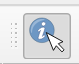
\includegraphics[width=0.28125in,height=\textheight]{images/clipboard-1450729439.png}
    tool located in the upper right of QGIS to retrieve RGB values for
    the following areas. Once you have filled in the table, discuss why
    you think different landcovers have different pixel values.

    \begin{longtable}[]{@{}
      >{\raggedright\arraybackslash}p{(\columnwidth - 10\tabcolsep) * \real{0.1139}}
      >{\raggedright\arraybackslash}p{(\columnwidth - 10\tabcolsep) * \real{0.1013}}
      >{\raggedright\arraybackslash}p{(\columnwidth - 10\tabcolsep) * \real{0.1392}}
      >{\raggedright\arraybackslash}p{(\columnwidth - 10\tabcolsep) * \real{0.2025}}
      >{\raggedright\arraybackslash}p{(\columnwidth - 10\tabcolsep) * \real{0.2278}}
      >{\raggedright\arraybackslash}p{(\columnwidth - 10\tabcolsep) * \real{0.2152}}@{}}
    \caption{Pixel brightness values for different land cover types in
    MKRF}\tabularnewline
    \toprule\noalign{}
    \begin{minipage}[b]{\linewidth}\raggedright
    E
    \end{minipage} & \begin{minipage}[b]{\linewidth}\raggedright
    N
    \end{minipage} & \begin{minipage}[b]{\linewidth}\raggedright
    Landcover
    \end{minipage} & \begin{minipage}[b]{\linewidth}\raggedright
    Red Brightness
    \end{minipage} & \begin{minipage}[b]{\linewidth}\raggedright
    Green Brightness
    \end{minipage} & \begin{minipage}[b]{\linewidth}\raggedright
    Blue Brightness
    \end{minipage} \\
    \midrule\noalign{}
    \endfirsthead
    \toprule\noalign{}
    \begin{minipage}[b]{\linewidth}\raggedright
    E
    \end{minipage} & \begin{minipage}[b]{\linewidth}\raggedright
    N
    \end{minipage} & \begin{minipage}[b]{\linewidth}\raggedright
    Landcover
    \end{minipage} & \begin{minipage}[b]{\linewidth}\raggedright
    Red Brightness
    \end{minipage} & \begin{minipage}[b]{\linewidth}\raggedright
    Green Brightness
    \end{minipage} & \begin{minipage}[b]{\linewidth}\raggedright
    Blue Brightness
    \end{minipage} \\
    \midrule\noalign{}
    \endhead
    \bottomrule\noalign{}
    \endlastfoot
    1248400 & 481890 & & & & \\
    1247760 & 848198 & & & & \\
    1248195 & 483318 & & & & \\
    1247019 & 483138 & & & & \\
    \end{longtable}
  \item[$\square$]
    Question 7: When you look at a clear cut area, what characteristics
    support an area is harvested? Consider size, shape, texture,
    proximity to other features, etc. List three specific
    characteristics to identify a harvested area that you could give to
    someone else who has never seen an above view of a clear cut.
  \item[$\square$]
    Question 8: Create a reference table that describes specific
    characteristics that can help differentiate land cover types using
    aerial imagery. For each feature in the below table include 3
    characteristics of the different land covers.
  \item[$\square$]
    Question 9: How do values for your different forest polygons layer
    differ in terms of brightness? What feature had the highest
    greenness reflectance? Which feature had the most variable greenness
    reflectance? Use values to support your results.
  \item[$\square$]
    Question 10: Normally, photo-interpreters would have a 3-D view of a
    stereo-pair of photos and they could see and measure stand heights.
    What other information might help the photo-interpreter assign
    heights to each stand?~ HINTS: As well as imagery, what other
    information might they access? How do other attributes impact
    height?
  \item[$\square$]
    Question 11: If you were monitoring a forest area for \ul{harvest
    disturbances}, would you choose to get new aerial photographs or
    would you use available Landsat data? Consider \ul{the costs, the
    spatial resolution of the images relative to the disturbance size,
    and the frequency that images are acquired}.
  \item[$\square$]
    Question 12. What about using landsat data for something like
    small-scale wind damage? Or small-scale fires? What about roads?
  \end{itemize}
\item[$\square$]
  Complete Maps for :

  \begin{itemize}
  \tightlist
  \item[$\square$]
    Your photo-interpreted forest polygons. Include the mean and
    standard deviation for the green birghtness values form the 2006
    orthomosaic.
  \item
    Make sure that your map includes:

    \begin{itemize}
    \tightlist
    \item
      A title
    \item
      A scale bar
    \item
      A north arrow
    \item
      A proper legend
    \end{itemize}
  \end{itemize}
\end{itemize}

\hypertarget{summary-1}{%
\section*{Summary}\label{summary-1}}
\addcontentsline{toc}{section}{Summary}

\markright{Summary}

\bookmarksetup{startatroot}

\hypertarget{terrain-spatial-interpolation}{%
\chapter{Exercise 3: Simple Sampling
Designs}\label{terrain-spatial-interpolation}}

Written by

Sarah Smith-Tripp

\hypertarget{lab-overview-2}{%
\section*{Lab Overview}\label{lab-overview-2}}
\addcontentsline{toc}{section}{Lab Overview}

\markright{Lab Overview}

This lab uses a ``simulated'' forest to practice simple random sampling,
summarizing the data, and then using that information as we would in a
real forest environment. We will use this sample data to estimate
important forest metrics and confidence around our estimates.

\begin{center}\rule{0.5\linewidth}{0.5pt}\end{center}

\hypertarget{learning-objectives-2}{%
\section*{Learning Objectives}\label{learning-objectives-2}}
\addcontentsline{toc}{section}{Learning Objectives}

\markright{Learning Objectives}

\begin{itemize}
\item
  Estimate the population mean and the confidence intervals using simple
  random sampling
\item
  Apply estimates + confidence intervals to answer management questions
\item
  Apply a systematic sampling design to estimate population mean and
  confidence intervals
\item
  Compare the cost and relative efficacy of different sampling regimes.
\end{itemize}

\begin{tcolorbox}[enhanced jigsaw, colbacktitle=quarto-callout-note-color!10!white, leftrule=.75mm, left=2mm, opacitybacktitle=0.6, breakable, colframe=quarto-callout-note-color-frame, arc=.35mm, bottomtitle=1mm, rightrule=.15mm, title=\textcolor{quarto-callout-note-color}{\faInfo}\hspace{0.5em}{Note}, toptitle=1mm, titlerule=0mm, opacityback=0, coltitle=black, colback=white, bottomrule=.15mm, toprule=.15mm]

Prior to completing this exercise go over the terminology and equations
included the course lecture material. It is important to know what a
\emph{population} mean is and how we describe this using
\emph{estimators}

\end{tcolorbox}

\hypertarget{data-overview}{%
\section*{Data Overview}\label{data-overview}}
\addcontentsline{toc}{section}{Data Overview}

\markright{Data Overview}

\includegraphics{03-Simple-Sampling-Design_files/figure-pdf/unnamed-chunk-4-1.pdf}

\begin{center}\rule{0.5\linewidth}{0.5pt}\end{center}

\hypertarget{task-1-simple-random-sampling}{%
\section*{Task 1: Simple Random
Sampling}\label{task-1-simple-random-sampling}}
\addcontentsline{toc}{section}{Task 1: Simple Random Sampling}

\markright{Task 1: Simple Random Sampling}

\textbf{Step 1}

\hypertarget{question-1-2}{%
\subsection*{Question 1}\label{question-1-2}}
\addcontentsline{toc}{subsection}{Question 1}

Using the map above select n=15 plots using simple random sampling
without replacement. Explain how you used \textbf{simple random sampling
replacement to select the data}. How did you choose random numbers?

\begin{Shaded}
\begin{Highlighting}[]
\DocumentationTok{\#\# develop a sample }
\NormalTok{plot\_sample }\OtherTok{\textless{}{-}} \FunctionTok{sample}\NormalTok{(}\AttributeTok{x =} \DecValTok{1}\SpecialCharTok{:}\DecValTok{112}\NormalTok{, }\AttributeTok{size =} \DecValTok{15}\NormalTok{, }\AttributeTok{replace =}\NormalTok{ F)}
\end{Highlighting}
\end{Shaded}

\hypertarget{question-2-2}{%
\subsection*{Question 2}\label{question-2-2}}
\addcontentsline{toc}{subsection}{Question 2}

Calculate:

\begin{enumerate}
\def\labelenumi{\arabic{enumi}.}
\tightlist
\item
  Mean volume per plot
\item
  The estimated plot-to-plot variance
\item
  The estimated variance of the mean (remember that this is sampling
  without replacement)
\item
  The estimated standard error of the mean
\item
  95\% confidence interval for this mean.
\end{enumerate}

\begin{tcolorbox}[enhanced jigsaw, colbacktitle=quarto-callout-note-color!10!white, leftrule=.75mm, left=2mm, opacitybacktitle=0.6, breakable, colframe=quarto-callout-note-color-frame, arc=.35mm, bottomtitle=1mm, rightrule=.15mm, title=\textcolor{quarto-callout-note-color}{\faInfo}\hspace{0.5em}{Note}, toptitle=1mm, titlerule=0mm, opacityback=0, coltitle=black, colback=white, bottomrule=.15mm, toprule=.15mm]

\emph{You must should calculations and include measurement units in your
responses. For your confidence interval calculation, shot is a range
with the lower value first.}

\end{tcolorbox}

\hypertarget{question-3-2}{%
\subsection*{Question 3}\label{question-3-2}}
\addcontentsline{toc}{subsection}{Question 3}

Convert the estimated mean volume per plot and the associated confidence
interval to an equivalent per hectare estimate (e.g.~200m3/ha with a
confidence interval of (100 m3/ha)

\hypertarget{question-4-2}{%
\subsection*{Question 4}\label{question-4-2}}
\addcontentsline{toc}{subsection}{Question 4}

Based on the volume per ha values, where in BC might these data have
come from? Consider (1) ecosystem type (2) time since disturbances. To
provide context, a very productive old stand in the Boreal Forest of
Canada could have up to 500 m\textsuperscript{3}/ha (most are much
less). A very productive old stand in the Temperate Rainforest of the
western coast of Canada could have 1,500 m\textsuperscript{3}/ha. Also,
1 m\textsuperscript{3} is about the size of a utility pole (e.g.,
telephone or electricity pole).

\hypertarget{question-5-2}{%
\subsection*{Question 5}\label{question-5-2}}
\addcontentsline{toc}{subsection}{Question 5}

How large is total plot area in hectares (you determined this in
Activity 3 already)? Use this to expand the mean in
m\textsuperscript{3}/ha and the associated confidence interval to obtain
the estimated total m\textsuperscript{3} volume for the land area and a
95\% confidence interval for this estimate. Based on this confidence
interval, would you say that there could be 3000 m\textsuperscript{3} of
volume in this area?

\hypertarget{question-6-1}{%
\subsection*{Question 6}\label{question-6-1}}
\addcontentsline{toc}{subsection}{Question 6}

Calculate the Percent Error achieved for your survey. Did you achieve
the desired percent error of~ + or -- 15\% of the mean with 95\%
probability? NOTE: This is the standard for operational cruising in BC
for scale-based sales (i.e., billing is based on scaled logs not on
standing estimated cruise volumes).

\begin{center}\rule{0.5\linewidth}{0.5pt}\end{center}

\hypertarget{task-2-systematic-random-sampling}{%
\section*{Task 2: Systematic Random
Sampling}\label{task-2-systematic-random-sampling}}
\addcontentsline{toc}{section}{Task 2: Systematic Random Sampling}

\markright{Task 2: Systematic Random Sampling}

For the following questions imaging a forester is planning a survey with
the with the following specifications:

\begin{enumerate}
\def\labelenumi{\Alph{enumi}.}
\item
  Intensity (\emph{I}) = 0.02 (i.e., 2 \%)
\item
  Forest land area (\emph{A}) = 100 ha (1000 m X 1000 m; 1 ha = 10,000
  m\textsuperscript{2})
\item
  Size of plot (\emph{a})= 0.02 ha (i.e., 14.14 X 14.14 square plot)
\end{enumerate}

\hypertarget{question-7-1}{%
\subsection*{Question 7}\label{question-7-1}}
\addcontentsline{toc}{subsection}{Question 7}

A. The area of the all of the plots of that will be needed for this
forester's survey using this intensity (A\emph{p}); and B. The number of
samples (\emph{n}) required for this desired sampling intensity, given
the specified plot size.

\hypertarget{question-8-2}{%
\subsection*{Question 8}\label{question-8-2}}
\addcontentsline{toc}{subsection}{Question 8}

Given that the length between plot centres (\emph{B}) is fixed at 40 m,
what is the length between lines (\emph{L})?~\textbf{NOTE: In practice,
we would round down to the nearest 5 m to lay this out in the field}.
For example, if the answer was 103 m, we would use 40 m by 100 m spacing
(not 105 m and not 103 m spacing), since forest land areas are often
irregular in shape and this would ``pull in'' the systematic sampling
grid to hopefully get enough plots.

What would the spacing be, if this square spacing between plot centres
was used instead? Again, in practice, we would round this answer down to
the nearest 5 m to lay this out in the field.

Which of these two options would you choose to use and why?

\hypertarget{question-9-2}{%
\subsection*{Question 9}\label{question-9-2}}
\addcontentsline{toc}{subsection}{Question 9}

Using the square spacing calculated in 2b and the plot size, select
random co-ordinates for you first plot centre in the first ``grid'' of
your systematic survey. Show all calculations you used to get the random
co-ordinates and to make sure that the plot will fit within the first
``grid square'' of your systematic survey given these random
co-ordinates and the plot dimensions.

\hypertarget{question-10-2}{%
\subsection*{Question 10}\label{question-10-2}}
\addcontentsline{toc}{subsection}{Question 10}

Given a fixed project cost of \$5,000 (i.e., truck rental and other
equipment) and a per day cost of \$1,000 for a 2-person crew with a
production rate of eight plots per day: A. How long would the survey
take? B. What would the cost of this survey be?

\hypertarget{question-11-2}{%
\subsection*{Question 11}\label{question-11-2}}
\addcontentsline{toc}{subsection}{Question 11}

if the budget was set at \$10,000:

A.How many plots could you have measured using the cost estimates in
\#10? B. What would the sampling intensity be for this fixed budget? C.
Would this sampling intensity be more or less than the sampling
intensity used in the sample plan (i.e., planned for 2\%)?

\begin{center}\rule{0.5\linewidth}{0.5pt}\end{center}

\hypertarget{lab-questions-deliverables-2}{%
\section*{Lab Questions \&
Deliverables}\label{lab-questions-deliverables-2}}
\addcontentsline{toc}{section}{Lab Questions \& Deliverables}

\markright{Lab Questions \& Deliverables}

\begin{itemize}
\tightlist
\item[$\square$]
  Complete answers for all 11 following questions:

  \begin{itemize}
  \tightlist
  \item[$\square$]
    Questions should show all work including calculations
  \item[$\square$]
    If you used code, make sure to include the code you used to answer
    the question.
  \end{itemize}
\end{itemize}

\hypertarget{summary-2}{%
\section*{Summary}\label{summary-2}}
\addcontentsline{toc}{section}{Summary}

\markright{Summary}

In this lab, we practiced the calculations of important summary
statistics from a random sampling design. We also learned and applied
our investigation to look at sampling intensity in systematic random
sampling.

\bookmarksetup{startatroot}

\hypertarget{compilation-of-fixed-area-plots-to-a-stand-level}{%
\chapter{04 - Compilation of Fixed-Area Plots to a Stand
Level}\label{compilation-of-fixed-area-plots-to-a-stand-level}}

Written by

Sarah Smith-Tripp

\hypertarget{lab-overview-3}{%
\section*{Lab Overview}\label{lab-overview-3}}
\addcontentsline{toc}{section}{Lab Overview}

\markright{Lab Overview}

This lab builds on our previous work to introduce more stand-level
summaries as well as using forest data to summarize important forest
attributes like volume and biomass. You will work with formulas, created
from test data, to understand a forest-stand. Using your estimates you
will produce a data summary for a landowner. You may work in groups for
this lab, but each student must be able to run the code on their own
computer.

\begin{center}\rule{0.5\linewidth}{0.5pt}\end{center}

\hypertarget{learning-objectives-3}{%
\section*{Learning Objectives}\label{learning-objectives-3}}
\addcontentsline{toc}{section}{Learning Objectives}

\markright{Learning Objectives}

\begin{itemize}
\item
  Practice analysis of fixed-area plots to obtain plot summaries.
\item
  Use simple random sampling to summarize plot-level data to obtain a
  stand-level summary
\item
  Summarize tree-level data to obtain plot-level stand and stock tables.
  Use this tree level data to obtain stand-level stock and stand tables
\end{itemize}

\hypertarget{problem-introduction}{%
\section*{Problem Introduction}\label{problem-introduction}}
\addcontentsline{toc}{section}{Problem Introduction}

\markright{Problem Introduction}

\textbf{General Description}

A landowner hires you to conduct a survey of a 30-ha forested parcel of
land (BC Coast).~In particular, the owner would like to know how much
they could make on the carbon market if they kept this forest intact and
sold the carbon credits.~From reading several documents, you find out
that: 1) about 50\% of aboveground biomass is carbon; and 2) the rate
for carbon credits is about \$65 CAD per C tonne. The owner would also
like to know general information about the timber characteristics for
general management purposes.

\begin{center}\rule{0.5\linewidth}{0.5pt}\end{center}

\hypertarget{key-formulas}{%
\section*{Key Formulas}\label{key-formulas}}
\addcontentsline{toc}{section}{Key Formulas}

\markright{Key Formulas}

For today's data investigation we will use formulas created by the
ministry to calculate volume and dry biomass for different tree species
in British Columbia. The coefficients are described in the table below.
Models for volume use Schumaker's volume function.

\$\$ Volume(m\^{}3) = 10\^{}\{(A +B(Log\_\{10\}(DBH(cm))) +
C*(Log\_\{10\}(Height(m))))\}\$\$

\global\setlength{\Oldarrayrulewidth}{\arrayrulewidth}

\global\setlength{\Oldtabcolsep}{\tabcolsep}

\setlength{\tabcolsep}{2pt}

\renewcommand*{\arraystretch}{1.5}



\providecommand{\ascline}[3]{\noalign{\global\arrayrulewidth #1}\arrayrulecolor[HTML]{#2}\cline{#3}}

\begin{longtable}[c]{|p{1.00in}|p{2.19in}|p{0.97in}|p{0.84in}|p{0.92in}}
\caption{BC Ministry of Forest Volume Coefficients}\tabularnewline




\ascline{1.5pt}{666666}{1-5}

\multicolumn{1}{>{\raggedright}m{\dimexpr 1in+0\tabcolsep}}{\textcolor[HTML]{000000}{\fontsize{11}{11}\selectfont{\global\setmainfont{Arial}{\textbf{Type}}}}} & \multicolumn{1}{>{\raggedright}m{\dimexpr 2.19in+0\tabcolsep}}{\textcolor[HTML]{000000}{\fontsize{11}{11}\selectfont{\global\setmainfont{Arial}{\textbf{Tree\ Types}}}}} & \multicolumn{1}{>{\raggedleft}m{\dimexpr 0.97in+0\tabcolsep}}{\textcolor[HTML]{000000}{\fontsize{11}{11}\selectfont{\global\setmainfont{Arial}{\textbf{A}}}}} & \multicolumn{1}{>{\raggedleft}m{\dimexpr 0.84in+0\tabcolsep}}{\textcolor[HTML]{000000}{\fontsize{11}{11}\selectfont{\global\setmainfont{Arial}{\textbf{B}}}}} & \multicolumn{1}{>{\raggedleft}m{\dimexpr 0.92in+0\tabcolsep}}{\textcolor[HTML]{000000}{\fontsize{11}{11}\selectfont{\global\setmainfont{Arial}{\textbf{C}}}}} \\

\ascline{1.5pt}{666666}{1-5}\endfirsthead 

\ascline{1.5pt}{666666}{1-5}

\multicolumn{1}{>{\raggedright}m{\dimexpr 1in+0\tabcolsep}}{\textcolor[HTML]{000000}{\fontsize{11}{11}\selectfont{\global\setmainfont{Arial}{\textbf{Type}}}}} & \multicolumn{1}{>{\raggedright}m{\dimexpr 2.19in+0\tabcolsep}}{\textcolor[HTML]{000000}{\fontsize{11}{11}\selectfont{\global\setmainfont{Arial}{\textbf{Tree\ Types}}}}} & \multicolumn{1}{>{\raggedleft}m{\dimexpr 0.97in+0\tabcolsep}}{\textcolor[HTML]{000000}{\fontsize{11}{11}\selectfont{\global\setmainfont{Arial}{\textbf{A}}}}} & \multicolumn{1}{>{\raggedleft}m{\dimexpr 0.84in+0\tabcolsep}}{\textcolor[HTML]{000000}{\fontsize{11}{11}\selectfont{\global\setmainfont{Arial}{\textbf{B}}}}} & \multicolumn{1}{>{\raggedleft}m{\dimexpr 0.92in+0\tabcolsep}}{\textcolor[HTML]{000000}{\fontsize{11}{11}\selectfont{\global\setmainfont{Arial}{\textbf{C}}}}} \\

\ascline{1.5pt}{666666}{1-5}\endhead



\multicolumn{1}{>{\raggedright}m{\dimexpr 1in+0\tabcolsep}}{\textcolor[HTML]{000000}{\fontsize{11}{11}\selectfont{\global\setmainfont{Arial}{BC}}}\textcolor[HTML]{000000}{\fontsize{11}{11}\selectfont{\global\setmainfont{Arial}{\linebreak }}}\textcolor[HTML]{000000}{\fontsize{11}{11}\selectfont{\global\setmainfont{Arial}{Traditional}}}} & \multicolumn{1}{>{\raggedright}m{\dimexpr 2.19in+0\tabcolsep}}{\textcolor[HTML]{000000}{\fontsize{11}{11}\selectfont{\global\setmainfont{Arial}{}}}} & \multicolumn{1}{>{\raggedleft}m{\dimexpr 0.97in+0\tabcolsep}}{\textcolor[HTML]{000000}{\fontsize{11}{11}\selectfont{\global\setmainfont{Arial}{}}}} & \multicolumn{1}{>{\raggedleft}m{\dimexpr 0.84in+0\tabcolsep}}{\textcolor[HTML]{000000}{\fontsize{11}{11}\selectfont{\global\setmainfont{Arial}{}}}} & \multicolumn{1}{>{\raggedleft}m{\dimexpr 0.92in+0\tabcolsep}}{\textcolor[HTML]{000000}{\fontsize{11}{11}\selectfont{\global\setmainfont{Arial}{}}}} \\

\ascline{0.75pt}{666666}{1-5}



\multicolumn{1}{>{\raggedright}m{\dimexpr 1in+0\tabcolsep}}{\textcolor[HTML]{000000}{\fontsize{11}{11}\selectfont{\global\setmainfont{Arial}{}}}} & \multicolumn{1}{>{\raggedright}m{\dimexpr 2.19in+0\tabcolsep}}{\textcolor[HTML]{000000}{\fontsize{11}{11}\selectfont{\global\setmainfont{Arial}{immature\ western\ red\ cedar}}}} & \multicolumn{1}{>{\raggedleft}m{\dimexpr 0.97in+0\tabcolsep}}{\textcolor[HTML]{000000}{\fontsize{11}{11}\selectfont{\global\setmainfont{Arial}{4.139118}}}} & \multicolumn{1}{>{\raggedleft}m{\dimexpr 0.84in+0\tabcolsep}}{\textcolor[HTML]{000000}{\fontsize{11}{11}\selectfont{\global\setmainfont{Arial}{1.71677}}}} & \multicolumn{1}{>{\raggedleft}m{\dimexpr 0.92in+0\tabcolsep}}{\textcolor[HTML]{000000}{\fontsize{11}{11}\selectfont{\global\setmainfont{Arial}{1.047420}}}} \\

\ascline{0.75pt}{666666}{1-5}



\multicolumn{1}{>{\raggedright}m{\dimexpr 1in+0\tabcolsep}}{\textcolor[HTML]{000000}{\fontsize{11}{11}\selectfont{\global\setmainfont{Arial}{}}}} & \multicolumn{1}{>{\raggedright}m{\dimexpr 2.19in+0\tabcolsep}}{\textcolor[HTML]{000000}{\fontsize{11}{11}\selectfont{\global\setmainfont{Arial}{immature\ western\ hemlock}}}} & \multicolumn{1}{>{\raggedleft}m{\dimexpr 0.97in+0\tabcolsep}}{\textcolor[HTML]{000000}{\fontsize{11}{11}\selectfont{\global\setmainfont{Arial}{-4.418820}}}} & \multicolumn{1}{>{\raggedleft}m{\dimexpr 0.84in+0\tabcolsep}}{\textcolor[HTML]{000000}{\fontsize{11}{11}\selectfont{\global\setmainfont{Arial}{1.86778}}}} & \multicolumn{1}{>{\raggedleft}m{\dimexpr 0.92in+0\tabcolsep}}{\textcolor[HTML]{000000}{\fontsize{11}{11}\selectfont{\global\setmainfont{Arial}{1.099890}}}} \\

\ascline{0.75pt}{666666}{1-5}



\multicolumn{1}{>{\raggedright}m{\dimexpr 1in+0\tabcolsep}}{\textcolor[HTML]{000000}{\fontsize{11}{11}\selectfont{\global\setmainfont{Arial}{}}}} & \multicolumn{1}{>{\raggedright}m{\dimexpr 2.19in+0\tabcolsep}}{\textcolor[HTML]{000000}{\fontsize{11}{11}\selectfont{\global\setmainfont{Arial}{immature\ douglas\ fir}}}} & \multicolumn{1}{>{\raggedleft}m{\dimexpr 0.97in+0\tabcolsep}}{\textcolor[HTML]{000000}{\fontsize{11}{11}\selectfont{\global\setmainfont{Arial}{-4.319071}}}} & \multicolumn{1}{>{\raggedleft}m{\dimexpr 0.84in+0\tabcolsep}}{\textcolor[HTML]{000000}{\fontsize{11}{11}\selectfont{\global\setmainfont{Arial}{1.81382}}}} & \multicolumn{1}{>{\raggedleft}m{\dimexpr 0.92in+0\tabcolsep}}{\textcolor[HTML]{000000}{\fontsize{11}{11}\selectfont{\global\setmainfont{Arial}{1.042420}}}} \\

\ascline{0.75pt}{666666}{1-5}



\multicolumn{1}{>{\raggedright}m{\dimexpr 1in+0\tabcolsep}}{\textcolor[HTML]{000000}{\fontsize{11}{11}\selectfont{\global\setmainfont{Arial}{}}}} & \multicolumn{1}{>{\raggedright}m{\dimexpr 2.19in+0\tabcolsep}}{\textcolor[HTML]{000000}{\fontsize{11}{11}\selectfont{\global\setmainfont{Arial}{mature\ western\ red\ cedar}}}} & \multicolumn{1}{>{\raggedleft}m{\dimexpr 0.97in+0\tabcolsep}}{\textcolor[HTML]{000000}{\fontsize{11}{11}\selectfont{\global\setmainfont{Arial}{-4.103107}}}} & \multicolumn{1}{>{\raggedleft}m{\dimexpr 0.84in+0\tabcolsep}}{\textcolor[HTML]{000000}{\fontsize{11}{11}\selectfont{\global\setmainfont{Arial}{1.74324}}}} & \multicolumn{1}{>{\raggedleft}m{\dimexpr 0.92in+0\tabcolsep}}{\textcolor[HTML]{000000}{\fontsize{11}{11}\selectfont{\global\setmainfont{Arial}{0.981729}}}} \\

\ascline{0.75pt}{666666}{1-5}



\multicolumn{1}{>{\raggedright}m{\dimexpr 1in+0\tabcolsep}}{\textcolor[HTML]{000000}{\fontsize{11}{11}\selectfont{\global\setmainfont{Arial}{}}}} & \multicolumn{1}{>{\raggedright}m{\dimexpr 2.19in+0\tabcolsep}}{\textcolor[HTML]{000000}{\fontsize{11}{11}\selectfont{\global\setmainfont{Arial}{mature\ western\ hemlock}}}} & \multicolumn{1}{>{\raggedleft}m{\dimexpr 0.97in+0\tabcolsep}}{\textcolor[HTML]{000000}{\fontsize{11}{11}\selectfont{\global\setmainfont{Arial}{-4.337400}}}} & \multicolumn{1}{>{\raggedleft}m{\dimexpr 0.84in+0\tabcolsep}}{\textcolor[HTML]{000000}{\fontsize{11}{11}\selectfont{\global\setmainfont{Arial}{1.78350}}}} & \multicolumn{1}{>{\raggedleft}m{\dimexpr 0.92in+0\tabcolsep}}{\textcolor[HTML]{000000}{\fontsize{11}{11}\selectfont{\global\setmainfont{Arial}{1.120230}}}} \\

\ascline{0.75pt}{666666}{1-5}



\multicolumn{1}{>{\raggedright}m{\dimexpr 1in+0\tabcolsep}}{\textcolor[HTML]{000000}{\fontsize{11}{11}\selectfont{\global\setmainfont{Arial}{}}}} & \multicolumn{1}{>{\raggedright}m{\dimexpr 2.19in+0\tabcolsep}}{\textcolor[HTML]{000000}{\fontsize{11}{11}\selectfont{\global\setmainfont{Arial}{mature\ douglas\ fir}}}} & \multicolumn{1}{>{\raggedleft}m{\dimexpr 0.97in+0\tabcolsep}}{\textcolor[HTML]{000000}{\fontsize{11}{11}\selectfont{\global\setmainfont{Arial}{-4.348375}}}} & \multicolumn{1}{>{\raggedleft}m{\dimexpr 0.84in+0\tabcolsep}}{\textcolor[HTML]{000000}{\fontsize{11}{11}\selectfont{\global\setmainfont{Arial}{1.69244}}}} & \multicolumn{1}{>{\raggedleft}m{\dimexpr 0.92in+0\tabcolsep}}{\textcolor[HTML]{000000}{\fontsize{11}{11}\selectfont{\global\setmainfont{Arial}{1.181970}}}} \\

\ascline{0.75pt}{666666}{1-5}



\multicolumn{1}{>{\raggedright}m{\dimexpr 1in+0\tabcolsep}}{\textcolor[HTML]{000000}{\fontsize{11}{11}\selectfont{\global\setmainfont{Arial}{}}}} & \multicolumn{1}{>{\raggedright}m{\dimexpr 2.19in+0\tabcolsep}}{\textcolor[HTML]{000000}{\fontsize{11}{11}\selectfont{\global\setmainfont{Arial}{red\ alder}}}} & \multicolumn{1}{>{\raggedleft}m{\dimexpr 0.97in+0\tabcolsep}}{\textcolor[HTML]{000000}{\fontsize{11}{11}\selectfont{\global\setmainfont{Arial}{-4.431705}}}} & \multicolumn{1}{>{\raggedleft}m{\dimexpr 0.84in+0\tabcolsep}}{\textcolor[HTML]{000000}{\fontsize{11}{11}\selectfont{\global\setmainfont{Arial}{1.77859}}}} & \multicolumn{1}{>{\raggedleft}m{\dimexpr 0.92in+0\tabcolsep}}{\textcolor[HTML]{000000}{\fontsize{11}{11}\selectfont{\global\setmainfont{Arial}{1.090770}}}} \\

\ascline{0.75pt}{666666}{1-5}



\multicolumn{1}{>{\raggedright}m{\dimexpr 1in+0\tabcolsep}}{\textcolor[HTML]{000000}{\fontsize{11}{11}\selectfont{\global\setmainfont{Arial}{}}}} & \multicolumn{1}{>{\raggedright}m{\dimexpr 2.19in+0\tabcolsep}}{\textcolor[HTML]{000000}{\fontsize{11}{11}\selectfont{\global\setmainfont{Arial}{bitter\ cherry}}}} & \multicolumn{1}{>{\raggedleft}m{\dimexpr 0.97in+0\tabcolsep}}{\textcolor[HTML]{000000}{\fontsize{11}{11}\selectfont{\global\setmainfont{Arial}{-4.431705}}}} & \multicolumn{1}{>{\raggedleft}m{\dimexpr 0.84in+0\tabcolsep}}{\textcolor[HTML]{000000}{\fontsize{11}{11}\selectfont{\global\setmainfont{Arial}{1.77859}}}} & \multicolumn{1}{>{\raggedleft}m{\dimexpr 0.92in+0\tabcolsep}}{\textcolor[HTML]{000000}{\fontsize{11}{11}\selectfont{\global\setmainfont{Arial}{1.090770}}}} \\

\ascline{1.5pt}{666666}{1-5}



\end{longtable}



\arrayrulecolor[HTML]{000000}

\global\setlength{\arrayrulewidth}{\Oldarrayrulewidth}

\global\setlength{\tabcolsep}{\Oldtabcolsep}

\renewcommand*{\arraystretch}{1}

The Biomass equations use the following formula:

\[
Biomass = Intercept+ Slope * DDH
\]

Where DDH is the diameter squared times the height of the tree. \[
DDH = (DBH(cm)/100)*(DBH(cm)/100)*Height(m) 
\]

\global\setlength{\Oldarrayrulewidth}{\arrayrulewidth}

\global\setlength{\Oldtabcolsep}{\tabcolsep}

\setlength{\tabcolsep}{2pt}

\renewcommand*{\arraystretch}{1.5}



\providecommand{\ascline}[3]{\noalign{\global\arrayrulewidth #1}\arrayrulecolor[HTML]{#2}\cline{#3}}

\begin{longtable*}[c]{|p{2.03in}|p{0.93in}|p{0.70in}}



\ascline{1.5pt}{666666}{1-3}

\multicolumn{1}{>{\raggedright}m{\dimexpr 2.03in+0\tabcolsep}}{\textcolor[HTML]{000000}{\fontsize{11}{11}\selectfont{\global\setmainfont{Arial}{\textbf{Tree\ Types}}}}} & \multicolumn{1}{>{\raggedleft}m{\dimexpr 0.93in+0\tabcolsep}}{\textcolor[HTML]{000000}{\fontsize{11}{11}\selectfont{\global\setmainfont{Arial}{\textbf{Intercept}}}}} & \multicolumn{1}{>{\raggedleft}m{\dimexpr 0.7in+0\tabcolsep}}{\textcolor[HTML]{000000}{\fontsize{11}{11}\selectfont{\global\setmainfont{Arial}{\textbf{Slope}}}}} \\

\ascline{1.5pt}{666666}{1-3}\endfirsthead 

\ascline{1.5pt}{666666}{1-3}

\multicolumn{1}{>{\raggedright}m{\dimexpr 2.03in+0\tabcolsep}}{\textcolor[HTML]{000000}{\fontsize{11}{11}\selectfont{\global\setmainfont{Arial}{\textbf{Tree\ Types}}}}} & \multicolumn{1}{>{\raggedleft}m{\dimexpr 0.93in+0\tabcolsep}}{\textcolor[HTML]{000000}{\fontsize{11}{11}\selectfont{\global\setmainfont{Arial}{\textbf{Intercept}}}}} & \multicolumn{1}{>{\raggedleft}m{\dimexpr 0.7in+0\tabcolsep}}{\textcolor[HTML]{000000}{\fontsize{11}{11}\selectfont{\global\setmainfont{Arial}{\textbf{Slope}}}}} \\

\ascline{1.5pt}{666666}{1-3}\endhead



\multicolumn{1}{>{\raggedright}m{\dimexpr 2.03in+0\tabcolsep}}{\textcolor[HTML]{000000}{\fontsize{11}{11}\selectfont{\global\setmainfont{Arial}{mature\ western\ red\ cedar}}}} & \multicolumn{1}{>{\raggedleft}m{\dimexpr 0.93in+0\tabcolsep}}{\textcolor[HTML]{000000}{\fontsize{11}{11}\selectfont{\global\setmainfont{Arial}{40.4}}}} & \multicolumn{1}{>{\raggedleft}m{\dimexpr 0.7in+0\tabcolsep}}{\textcolor[HTML]{000000}{\fontsize{11}{11}\selectfont{\global\setmainfont{Arial}{96.9}}}} \\

\ascline{0.75pt}{666666}{1-3}



\multicolumn{1}{>{\raggedright}m{\dimexpr 2.03in+0\tabcolsep}}{\textcolor[HTML]{000000}{\fontsize{11}{11}\selectfont{\global\setmainfont{Arial}{mature\ western\ hemlock}}}} & \multicolumn{1}{>{\raggedleft}m{\dimexpr 0.93in+0\tabcolsep}}{\textcolor[HTML]{000000}{\fontsize{11}{11}\selectfont{\global\setmainfont{Arial}{29.8}}}} & \multicolumn{1}{>{\raggedleft}m{\dimexpr 0.7in+0\tabcolsep}}{\textcolor[HTML]{000000}{\fontsize{11}{11}\selectfont{\global\setmainfont{Arial}{155.8}}}} \\

\ascline{0.75pt}{666666}{1-3}



\multicolumn{1}{>{\raggedright}m{\dimexpr 2.03in+0\tabcolsep}}{\textcolor[HTML]{000000}{\fontsize{11}{11}\selectfont{\global\setmainfont{Arial}{mature\ douglas\ fir}}}} & \multicolumn{1}{>{\raggedleft}m{\dimexpr 0.93in+0\tabcolsep}}{\textcolor[HTML]{000000}{\fontsize{11}{11}\selectfont{\global\setmainfont{Arial}{37.2}}}} & \multicolumn{1}{>{\raggedleft}m{\dimexpr 0.7in+0\tabcolsep}}{\textcolor[HTML]{000000}{\fontsize{11}{11}\selectfont{\global\setmainfont{Arial}{139.3}}}} \\

\ascline{0.75pt}{666666}{1-3}



\multicolumn{1}{>{\raggedright}m{\dimexpr 2.03in+0\tabcolsep}}{\textcolor[HTML]{000000}{\fontsize{11}{11}\selectfont{\global\setmainfont{Arial}{red\ alder}}}} & \multicolumn{1}{>{\raggedleft}m{\dimexpr 0.93in+0\tabcolsep}}{\textcolor[HTML]{000000}{\fontsize{11}{11}\selectfont{\global\setmainfont{Arial}{4.8}}}} & \multicolumn{1}{>{\raggedleft}m{\dimexpr 0.7in+0\tabcolsep}}{\textcolor[HTML]{000000}{\fontsize{11}{11}\selectfont{\global\setmainfont{Arial}{206.5}}}} \\

\ascline{0.75pt}{666666}{1-3}



\multicolumn{1}{>{\raggedright}m{\dimexpr 2.03in+0\tabcolsep}}{\textcolor[HTML]{000000}{\fontsize{11}{11}\selectfont{\global\setmainfont{Arial}{bitter\ cherry}}}} & \multicolumn{1}{>{\raggedleft}m{\dimexpr 0.93in+0\tabcolsep}}{\textcolor[HTML]{000000}{\fontsize{11}{11}\selectfont{\global\setmainfont{Arial}{4.8}}}} & \multicolumn{1}{>{\raggedleft}m{\dimexpr 0.7in+0\tabcolsep}}{\textcolor[HTML]{000000}{\fontsize{11}{11}\selectfont{\global\setmainfont{Arial}{206.5}}}} \\

\ascline{1.5pt}{666666}{1-3}



\end{longtable*}



\arrayrulecolor[HTML]{000000}

\global\setlength{\arrayrulewidth}{\Oldarrayrulewidth}

\global\setlength{\tabcolsep}{\Oldtabcolsep}

\renewcommand*{\arraystretch}{1}

\hypertarget{data-description}{%
\section*{Data Description}\label{data-description}}
\addcontentsline{toc}{section}{Data Description}

\markright{Data Description}

You decide to use a systematic sampling approach to determine plot
centres for \emph{n}=4 plots.~For each plot center, you establish a
circular, fixed-area plot (r=11.27 m; 0.04 ha) aiming to sample all
trees which are ≥ 2.0 cm DBH within this radius. Some plots had a lot of
trees and thus a process of ``Half Sweeps'' was conducted, where a
randomly chosen half of the 0.04 ha (or a slice) was selected and only
trees in that half of the plot were recorded (i.e., each tree counts
twice in the 0.04 ha plot OR the plot size was reduced to 0.02 ha).

For each tree (DBH≥2.0 cm) in the plot (full or half plot), the species
was recorded and the DBH (cm) was measured. On a subset of trees, the
height (m) was measured in the field. For the remaining trees, the
height was estimated in the office using existing height/DBH models
(i.e., for each tree without height, the species-specific models
developed for this area were used to estimate height from DBH). ~{[}For
broken trees,{]} the height to the break was measured in the field, and
an estimate of the height that the tree might have been if not broken
was also recorded in the field. A snapshot of these data are provided
below.

From these data, you determine the characteristics of the forest land
and report these to the landowner, along with your estimate of potential
carbon credits.

\begin{verbatim}
# A tibble: 4 x 3
  PlotNo number_trees plot_type
   <int>        <int> <chr>    
1      1           15 Half     
2      2           21 Full     
3      3           10 Half     
4      4           12 Full     
\end{verbatim}

\hypertarget{plot-level-analyses}{%
\section*{Plot Level Analyses}\label{plot-level-analyses}}
\addcontentsline{toc}{section}{Plot Level Analyses}

\markright{Plot Level Analyses}

Following the example code below (using fake data!) use the \emph{real}
data included in your lab exercises to calculate the average tree size
in terms of DBH, height and basal area per tree, total volume per tree,
and biomass. Remember to report the measurements units for each of these
metrics. The code below includes both a right and a wrong version. In
your analysis, discuss which version you used and why. Additionally,
there were some useful formulas created to analyse data in lab 3. We'll
be working work this code for our analyses.

\begin{Shaded}
\begin{Highlighting}[]
\FunctionTok{set.seed}\NormalTok{(}\DecValTok{1234}\NormalTok{)}
\CommentTok{\# load packages }
\FunctionTok{library}\NormalTok{(pacman)}
\FunctionTok{p\_load}\NormalTok{(tidyverse, ggplot2, dplyr)}
\DocumentationTok{\#\# set up some useful functions }
\DocumentationTok{\#\# variance around the maean }
\NormalTok{var\_simple\_random }\OtherTok{\textless{}{-}} \ControlFlowTok{function}\NormalTok{(data)\{}
\NormalTok{  ybar }\OtherTok{\textless{}{-}} \FunctionTok{mean}\NormalTok{(data, }\AttributeTok{na.rm =}\NormalTok{T) }\DocumentationTok{\#\# calculate the mean}
\NormalTok{  top\_sum }\OtherTok{\textless{}{-}} \FunctionTok{sum}\NormalTok{((data }\SpecialCharTok{{-}}\NormalTok{ ybar) }\SpecialCharTok{\^{}} \DecValTok{2}\NormalTok{)}
\NormalTok{  df }\OtherTok{\textless{}{-}} \FunctionTok{length}\NormalTok{(data)}
\NormalTok{  var\_simple }\OtherTok{\textless{}{-}}\NormalTok{ top\_sum}\SpecialCharTok{/}\NormalTok{ (df}\DecValTok{{-}1}\NormalTok{)}
  \FunctionTok{return}\NormalTok{(var\_simple)}
\NormalTok{\}}
\DocumentationTok{\#\# standard deviation w and without replacement }
\NormalTok{sd\_simple\_random }\OtherTok{\textless{}{-}} \ControlFlowTok{function}\NormalTok{(data, }\AttributeTok{replacement =}\NormalTok{ T, }\AttributeTok{N\_big =} \ConstantTok{NULL}\NormalTok{) \{}
\NormalTok{  ybar }\OtherTok{\textless{}{-}} \FunctionTok{mean}\NormalTok{(data, }\AttributeTok{na.rm =}\NormalTok{ T) }\DocumentationTok{\#\# calculate the mean}
\NormalTok{  top\_sum }\OtherTok{\textless{}{-}} \FunctionTok{sum}\NormalTok{((data }\SpecialCharTok{{-}}\NormalTok{ ybar) }\SpecialCharTok{\^{}} \DecValTok{2}\NormalTok{)}
\NormalTok{  df }\OtherTok{\textless{}{-}} \FunctionTok{length}\NormalTok{(data)}
\NormalTok{  var\_simple }\OtherTok{\textless{}{-}}\NormalTok{ top\_sum }\SpecialCharTok{/}\NormalTok{ (df }\SpecialCharTok{{-}} \DecValTok{1}\NormalTok{)}
  \ControlFlowTok{if}\NormalTok{ (replacement }\SpecialCharTok{==}\NormalTok{ F) \{}
    \DocumentationTok{\#\# adjustment neded to control for the limited sampel}
    \ControlFlowTok{if}\NormalTok{ (}\FunctionTok{length}\NormalTok{(N\_big) }\SpecialCharTok{==} \DecValTok{0}\NormalTok{) \{}
      \FunctionTok{return}\NormalTok{(}\StringTok{\textquotesingle{}Total Possible Needed\textquotesingle{}}\NormalTok{)}
\NormalTok{    \} }\ControlFlowTok{else} \ControlFlowTok{if}\NormalTok{ (}\FunctionTok{length}\NormalTok{(N\_big) }\SpecialCharTok{\textgreater{}} \DecValTok{0}\NormalTok{) \{}
\NormalTok{      adj\_fct }\OtherTok{\textless{}{-}}\NormalTok{ (N\_big }\SpecialCharTok{{-}}\NormalTok{ df) }\SpecialCharTok{/}\NormalTok{ N\_big}
\NormalTok{      sd\_mean }\OtherTok{=}\NormalTok{ (var\_simple }\SpecialCharTok{/}\NormalTok{ df) }\SpecialCharTok{*}\NormalTok{ adj\_fct}
      \FunctionTok{return}\NormalTok{(sd\_mean)}
\NormalTok{    \}}
\NormalTok{  \}}
  \ControlFlowTok{else}\NormalTok{ \{}
\NormalTok{    sd\_mean }\OtherTok{=}\NormalTok{ var\_simple }\SpecialCharTok{/}\NormalTok{ df}
    \FunctionTok{return}\NormalTok{(sd\_mean)}
\NormalTok{  \}}
\NormalTok{\}}
\DocumentationTok{\#\# confidence intervals for mean of population}
\NormalTok{confident\_interval }\OtherTok{\textless{}{-}} \ControlFlowTok{function}\NormalTok{(x, }\AttributeTok{alpha =} \FloatTok{0.05}\NormalTok{)\{}
\NormalTok{  n }\OtherTok{\textless{}{-}} \FunctionTok{length}\NormalTok{(x)}
\NormalTok{  mean\_x }\OtherTok{\textless{}{-}} \FunctionTok{mean}\NormalTok{(x, }\AttributeTok{na.rm =}\NormalTok{ T)}
  \DocumentationTok{\#\# this is the sd of the mean }
\NormalTok{  se }\OtherTok{\textless{}{-}} \FunctionTok{sd}\NormalTok{(x, }\AttributeTok{na.rm =}\NormalTok{T)}\SpecialCharTok{/}\FunctionTok{sqrt}\NormalTok{(n)}
\NormalTok{  t\_value }\OtherTok{\textless{}{-}} \FunctionTok{qt}\NormalTok{(}\DecValTok{1} \SpecialCharTok{{-}}\NormalTok{ alpha}\SpecialCharTok{/}\DecValTok{2}\NormalTok{, }\AttributeTok{df =}\NormalTok{ n }\SpecialCharTok{{-}} \DecValTok{1}\NormalTok{)}
  \DocumentationTok{\#\# confidence ofthe mean of the population}
\NormalTok{  ci }\OtherTok{\textless{}{-}}\NormalTok{ mean\_x }\SpecialCharTok{+} \FunctionTok{c}\NormalTok{(}\SpecialCharTok{{-}}\DecValTok{1}\NormalTok{, }\DecValTok{1}\NormalTok{) }\SpecialCharTok{*}\NormalTok{ t\_value }\SpecialCharTok{*}\NormalTok{ se}
  \FunctionTok{return}\NormalTok{(ci)}
\NormalTok{\}}
\NormalTok{new\_sample\_size }\OtherTok{\textless{}{-}} \ControlFlowTok{function}\NormalTok{(Allowable\_Error, }
\NormalTok{                            data,}
                            \AttributeTok{replacement =} \ConstantTok{TRUE}\NormalTok{,}
                            \AttributeTok{N =} \DecValTok{100}\NormalTok{) \{}
  \DocumentationTok{\#\# calculate confidence interval }
\NormalTok{  CI }\OtherTok{\textless{}{-}} \FunctionTok{confident\_interval}\NormalTok{(data)}
  
  \DocumentationTok{\#\# percent error }
\NormalTok{  PE }\OtherTok{\textless{}{-}}\NormalTok{ (}\FunctionTok{diff}\NormalTok{(CI) }\SpecialCharTok{*} \FloatTok{0.5}\NormalTok{) }\SpecialCharTok{/} \FunctionTok{mean}\NormalTok{(data) }\SpecialCharTok{*} \DecValTok{100}
  
  \DocumentationTok{\#\# calculate mean}
\NormalTok{  mean\_val }\OtherTok{\textless{}{-}} \FunctionTok{mean}\NormalTok{(data)}

  \CommentTok{\#test\_stat \textless{}{-} mean\_val {-} 0.95 / (var(data)\^{}0.5)}
\NormalTok{  t\_val }\OtherTok{\textless{}{-}} \FunctionTok{qt}\NormalTok{(}\FloatTok{0.95}\NormalTok{, }\AttributeTok{df =} \FunctionTok{length}\NormalTok{(data)}\SpecialCharTok{{-}}\DecValTok{1}\NormalTok{, }\AttributeTok{lower.tail =}\NormalTok{ T)}
\NormalTok{  t\_val}
\NormalTok{  sd\_ }\OtherTok{\textless{}{-}} \FunctionTok{sd}\NormalTok{(data)}
\NormalTok{  CV }\OtherTok{=}\NormalTok{ (sd\_ }\SpecialCharTok{/}\NormalTok{ mean\_val) }\SpecialCharTok{*} \DecValTok{100} 
  \ControlFlowTok{if}\NormalTok{ (replacement }\SpecialCharTok{==} \ConstantTok{FALSE}\NormalTok{) \{}
\NormalTok{    Q }\OtherTok{\textless{}{-}}\NormalTok{ Allowable\_Error}\SpecialCharTok{\^{}}\DecValTok{2} \SpecialCharTok{/}\NormalTok{ (t\_val}\SpecialCharTok{\^{}}\DecValTok{2} \SpecialCharTok{*}\NormalTok{ CV}\SpecialCharTok{\^{}}\DecValTok{2}\NormalTok{)}
\NormalTok{    n\_out }\OtherTok{\textless{}{-}} \DecValTok{1} \SpecialCharTok{/}\NormalTok{ ((}\DecValTok{1} \SpecialCharTok{/}\NormalTok{ N) }\SpecialCharTok{+}\NormalTok{ Q)}
\NormalTok{    n\_out}
\NormalTok{    \} }\ControlFlowTok{else}\NormalTok{ \{}
\NormalTok{    n\_out }\OtherTok{\textless{}{-}}\NormalTok{ (t\_val}\SpecialCharTok{\^{}}\DecValTok{2} \SpecialCharTok{*}\NormalTok{ CV}\SpecialCharTok{\^{}}\DecValTok{2}\NormalTok{)}\SpecialCharTok{/}\NormalTok{ Allowable\_Error}\SpecialCharTok{\^{}}\DecValTok{2}
\NormalTok{  \}}
  \FunctionTok{return}\NormalTok{(}\FunctionTok{round}\NormalTok{(n\_out))}
\NormalTok{\}}
\end{Highlighting}
\end{Shaded}

\hypertarget{first-we-will-calculate-the-tree-level-variables}{%
\subsubsection{First we will calculate the tree level
variables}\label{first-we-will-calculate-the-tree-level-variables}}

\begin{Shaded}
\begin{Highlighting}[]
\DocumentationTok{\#\# read in our data }
\NormalTok{plot\_data }\OtherTok{\textless{}{-}} \FunctionTok{read.csv}\NormalTok{(}\StringTok{"Lab4\_Plotdata.csv"}\NormalTok{)}
\DocumentationTok{\#\# we are using fake data here }
\NormalTok{species\_list }\OtherTok{\textless{}{-}} \FunctionTok{unique}\NormalTok{(plot\_data}\SpecialCharTok{$}\NormalTok{Species)}
\DocumentationTok{\#\# species mapping }
\NormalTok{species\_fullnames }\OtherTok{\textless{}{-}} \FunctionTok{c}\NormalTok{(}\StringTok{\textquotesingle{}Cw\textquotesingle{}}\OtherTok{=}\StringTok{\textquotesingle{}western redcedar\textquotesingle{}}\NormalTok{, }\StringTok{\textquotesingle{}Hw\textquotesingle{}}\OtherTok{=}\StringTok{\textquotesingle{}western hemlock\textquotesingle{}}\NormalTok{, }\StringTok{\textquotesingle{}Fd\textquotesingle{}}\OtherTok{=}\StringTok{\textquotesingle{}douglas fir\textquotesingle{}}\NormalTok{, }\StringTok{\textquotesingle{}Ra\textquotesingle{}}\OtherTok{=}\StringTok{\textquotesingle{}red alder\textquotesingle{}}\NormalTok{, }\StringTok{\textquotesingle{}Bc\textquotesingle{}}\OtherTok{=}\StringTok{\textquotesingle{}bitter cherry\textquotesingle{}}\NormalTok{)}
\DocumentationTok{\#\# convert species in the volume coefficients factor }
\DocumentationTok{\#\# assuming all trees are mature }
\FunctionTok{p\_load}\NormalTok{(stringr)}
\NormalTok{coeff\_vol\_bio\_mat }\OtherTok{\textless{}{-}} \FunctionTok{filter}\NormalTok{(volume\_df, }\FunctionTok{str\_starts}\NormalTok{(tree\_types, }\StringTok{"mature"}\NormalTok{) }\SpecialCharTok{\&}\NormalTok{ Type }\SpecialCharTok{==}
                          \StringTok{\textquotesingle{}BC}\SpecialCharTok{\textbackslash{}n}\StringTok{Traditional\textquotesingle{}}\NormalTok{) }\SpecialCharTok{\%\textgreater{}\%} 
  \FunctionTok{mutate}\NormalTok{(}\AttributeTok{short\_names =} \FunctionTok{case\_when}\NormalTok{(tree\_types }\SpecialCharTok{==} \StringTok{\textquotesingle{}mature western red cedar\textquotesingle{}} \SpecialCharTok{\textasciitilde{}} \StringTok{\textquotesingle{}Cw\textquotesingle{}}\NormalTok{,}
\NormalTok{                                 tree\_types }\SpecialCharTok{==} \StringTok{\textquotesingle{}mature western hemlock\textquotesingle{}} \SpecialCharTok{\textasciitilde{}} \StringTok{\textquotesingle{}Hw\textquotesingle{}}\NormalTok{, }
\NormalTok{                                 tree\_types }\SpecialCharTok{==} \StringTok{\textquotesingle{}mature douglas fir\textquotesingle{}} \SpecialCharTok{\textasciitilde{}} \StringTok{\textquotesingle{}Fd\textquotesingle{}}\NormalTok{)) }\SpecialCharTok{\%\textgreater{}\%} 
  \FunctionTok{left\_join}\NormalTok{(biomass\_df, }\AttributeTok{by =} \FunctionTok{c}\NormalTok{(}\StringTok{\textquotesingle{}tree\_types\textquotesingle{}} \OtherTok{=} \StringTok{\textquotesingle{}trees\_types\_biomass\textquotesingle{}}\NormalTok{))}

\DocumentationTok{\#\# create a random list of species}
\NormalTok{fake\_data }\OtherTok{\textless{}{-}} \FunctionTok{data.frame}\NormalTok{(}\AttributeTok{Species =} \FunctionTok{sample}\NormalTok{(species\_list, }\DecValTok{100}\NormalTok{, }\AttributeTok{replace =} \ConstantTok{TRUE}\NormalTok{), }
                        \AttributeTok{DBH =} \FunctionTok{rnorm}\NormalTok{(}\DecValTok{100}\NormalTok{, }\DecValTok{30}\NormalTok{, }\DecValTok{2}\NormalTok{),}
                        \AttributeTok{Height =} \FunctionTok{rnorm}\NormalTok{(}\DecValTok{100}\NormalTok{, }\DecValTok{25}\NormalTok{, }\DecValTok{5}\NormalTok{),}
                        \AttributeTok{PlotNo =} \FunctionTok{sample}\NormalTok{(}\DecValTok{1}\SpecialCharTok{:}\DecValTok{4}\NormalTok{, }\DecValTok{100}\NormalTok{, }\AttributeTok{replace =} \ConstantTok{TRUE}\NormalTok{),}
                        \AttributeTok{Partial =} \FunctionTok{sample}\NormalTok{(}\FunctionTok{c}\NormalTok{(}\StringTok{"Full"}\NormalTok{, }\StringTok{"Half"}\NormalTok{), }\DecValTok{100}\NormalTok{, }\AttributeTok{replace =} \ConstantTok{TRUE}\NormalTok{),}
                        \AttributeTok{Treeno =} \FunctionTok{seq}\NormalTok{(}\DecValTok{1}\NormalTok{, }\DecValTok{100}\NormalTok{, }\AttributeTok{by =} \DecValTok{1}\NormalTok{))}
\DocumentationTok{\#\# using fake data and the volume coefficients and the species fullnames calculate the volume for each tree}
\NormalTok{fake\_data\_calcs\_tree }\OtherTok{\textless{}{-}}\NormalTok{ fake\_data }\SpecialCharTok{\%\textgreater{}\%} \FunctionTok{left\_join}\NormalTok{(coeff\_vol\_bio\_mat, }\AttributeTok{by =} \FunctionTok{c}\NormalTok{(}\StringTok{"Species"}\OtherTok{=}\StringTok{"short\_names"}\NormalTok{))}\SpecialCharTok{\%\textgreater{}\%} 
  \FunctionTok{group\_by}\NormalTok{(Treeno) }\SpecialCharTok{\%\textgreater{}\%}
  \FunctionTok{mutate}\NormalTok{(}\AttributeTok{BA =}\NormalTok{ (}\FunctionTok{sqrt}\NormalTok{(DBH}\SpecialCharTok{/}\NormalTok{(}\DecValTok{2}\SpecialCharTok{*}\DecValTok{100}\NormalTok{)) }\SpecialCharTok{*}\NormalTok{ pi), }\CommentTok{\# basal area per tree}
         \AttributeTok{Vol =}\NormalTok{  (}\DecValTok{10}\SpecialCharTok{\^{}}\NormalTok{(A }\SpecialCharTok{+}\NormalTok{ (B}\SpecialCharTok{*}\FunctionTok{log10}\NormalTok{(DBH)) }\SpecialCharTok{+}\NormalTok{ (C}\SpecialCharTok{*}\FunctionTok{log10}\NormalTok{(Height)))),}\DocumentationTok{\#\# volume per tree}
         \AttributeTok{biomass =}\NormalTok{ int }\SpecialCharTok{+}\NormalTok{ (slope }\SpecialCharTok{*}\NormalTok{ ((DBH}\SpecialCharTok{/}\DecValTok{100}\NormalTok{)}\SpecialCharTok{\^{}}\DecValTok{2}\NormalTok{) }\SpecialCharTok{*}\NormalTok{ Height)) }\CommentTok{\#biomass per tree}
\FunctionTok{head}\NormalTok{(fake\_data\_calcs\_tree)}
\end{Highlighting}
\end{Shaded}

\begin{verbatim}
# A tibble: 6 x 16
# Groups:   Treeno [6]
  Species   DBH Height PlotNo Partial Treeno tree_types     A     B      C Type 
  <chr>   <dbl>  <dbl>  <int> <chr>    <dbl> <chr>      <dbl> <dbl>  <dbl> <chr>
1 DD       26.4   23.1      3 Half         1 <NA>       NA    NA    NA      <NA>
2 DD       28.8   25.5      2 Half         2 <NA>       NA    NA    NA      <NA>
3 Fd       27.8   33.2      4 Half         3 mature do~ -4.35  1.69  1.18  "BC\~
4 Fd       28.0   20.6      2 Half         4 mature do~ -4.35  1.69  1.18  "BC\~
5 Cw       29.7   25.6      4 Half         5 mature we~ -4.10  1.74  0.982 "BC\~
6 DD       31.1   31.8      1 Half         6 <NA>       NA    NA    NA      <NA>
# i 5 more variables: int <dbl>, slope <dbl>, BA <dbl>, Vol <dbl>,
#   biomass <dbl>
\end{verbatim}

\hypertarget{then-we-will-calculate-the-per-hectare-variables-for-each-tree}{%
\subsubsection{Then we will calculate the per hectare variables for each
tree}\label{then-we-will-calculate-the-per-hectare-variables-for-each-tree}}

\begin{Shaded}
\begin{Highlighting}[]
\DocumentationTok{\#\# option a }
\NormalTok{opt\_A\_pHa }\OtherTok{\textless{}{-}}\NormalTok{ fake\_data\_calcs\_tree }\SpecialCharTok{\%\textgreater{}\%} 
  \FunctionTok{mutate}\NormalTok{(}\AttributeTok{SPH =} \DecValTok{1}\SpecialCharTok{/}\FloatTok{0.04}\NormalTok{) }\SpecialCharTok{\%\textgreater{}\%} 
  \FunctionTok{group\_by}\NormalTok{(Treeno) }\SpecialCharTok{\%\textgreater{}\%} 
  \FunctionTok{mutate}\NormalTok{(}\AttributeTok{BA\_pHa =}\NormalTok{ BA }\SpecialCharTok{*}\NormalTok{ SPH, }
         \AttributeTok{Vol\_pHa =}\NormalTok{ Vol }\SpecialCharTok{*}\NormalTok{ SPH, }
         \AttributeTok{biomass\_pHa =}\NormalTok{ biomass }\SpecialCharTok{*}\NormalTok{ SPH) }
\CommentTok{\# option b }
\NormalTok{opt\_B\_pHa }\OtherTok{\textless{}{-}}\NormalTok{ fake\_data\_calcs\_tree }\SpecialCharTok{\%\textgreater{}\%} 
  \FunctionTok{mutate}\NormalTok{(}\AttributeTok{SPH =} \FunctionTok{ifelse}\NormalTok{(Partial }\SpecialCharTok{==} \StringTok{"Half"}\NormalTok{, }\DecValTok{1}\SpecialCharTok{/}\FloatTok{0.02}\NormalTok{, }\DecValTok{1}\SpecialCharTok{/}\FloatTok{0.04}\NormalTok{)) }\SpecialCharTok{\%\textgreater{}\%} 
  \FunctionTok{group\_by}\NormalTok{(Treeno) }\SpecialCharTok{\%\textgreater{}\%} 
  \FunctionTok{mutate}\NormalTok{(}\AttributeTok{BA\_pHa =}\NormalTok{ BA, }
         \AttributeTok{Vol\_pHa =}\NormalTok{ Vol, }
         \AttributeTok{biomass\_pHa =}\NormalTok{ biomass)}
\NormalTok{trees\_pHa }\OtherTok{\textless{}{-}}\NormalTok{ opt\_A\_pHa}
\end{Highlighting}
\end{Shaded}

\hypertarget{finally-we-can-calculate-the-plot-and-stand-level-variables}{%
\subsubsection{Finally, we can calculate the plot and stand-level
variables}\label{finally-we-can-calculate-the-plot-and-stand-level-variables}}

\begin{Shaded}
\begin{Highlighting}[]
\DocumentationTok{\#\# option a}
\NormalTok{opt\_A\_plot }\OtherTok{\textless{}{-}}\NormalTok{ opt\_A\_pHa }\SpecialCharTok{\%\textgreater{}\%} 
  \FunctionTok{group\_by}\NormalTok{(PlotNo) }\SpecialCharTok{\%\textgreater{}\%} 
  \FunctionTok{summarise}\NormalTok{(}\AttributeTok{mean\_DBH =} \FunctionTok{mean}\NormalTok{(DBH, }\AttributeTok{na.rm =}\NormalTok{ T), }
            \AttributeTok{mean\_Height =} \FunctionTok{mean}\NormalTok{(Height, }\AttributeTok{na.rm =}\NormalTok{ T), }
            \AttributeTok{mean\_BA =} \FunctionTok{mean}\NormalTok{(BA, }\AttributeTok{na.rm=}\NormalTok{ T), }
            \AttributeTok{mean\_Vol =} \FunctionTok{mean}\NormalTok{(Vol, }\AttributeTok{na.rm =}\NormalTok{T), }
            \AttributeTok{mean\_biomass =} \FunctionTok{mean}\NormalTok{(biomass, }\AttributeTok{na.rm =}\NormalTok{ T),}
            \AttributeTok{mean\_BApHa =} \FunctionTok{sum}\NormalTok{(BA\_pHa, }\AttributeTok{na.rm =}\NormalTok{T), }
            \AttributeTok{mean\_VolpHa =} \FunctionTok{sum}\NormalTok{(Vol\_pHa, }\AttributeTok{na.rm =}\NormalTok{ T),}
            \AttributeTok{mean\_biomass\_pHa =} \FunctionTok{sum}\NormalTok{(biomass\_pHa, }\AttributeTok{na.rm =}\NormalTok{ T)) }\SpecialCharTok{\%\textgreater{}\%} 
  \FunctionTok{summarise\_all}\NormalTok{(mean)}
\DocumentationTok{\#\# option b}
\NormalTok{opt\_B\_plot }\OtherTok{\textless{}{-}} \FunctionTok{ungroup}\NormalTok{(opt\_B\_pHa) }\SpecialCharTok{\%\textgreater{}\%} \DocumentationTok{\#\# ungroup data to calculate stand level means }
  \FunctionTok{mutate}\NormalTok{(}\AttributeTok{Adjst =} \FunctionTok{ifelse}\NormalTok{(Partial }\SpecialCharTok{==} \StringTok{"Half"}\NormalTok{, }\FloatTok{0.5}\NormalTok{, }\DecValTok{1}\NormalTok{)) }\SpecialCharTok{\%\textgreater{}\%}
  \FunctionTok{reframe}\NormalTok{(}\AttributeTok{mean\_DBH =} \FunctionTok{mean}\NormalTok{(DBH, }\AttributeTok{na.rm =}\NormalTok{ T), }
            \AttributeTok{mean\_Height =} \FunctionTok{mean}\NormalTok{(Height, }\AttributeTok{na.rm =}\NormalTok{ T), }
            \AttributeTok{mean\_BA =} \FunctionTok{mean}\NormalTok{(BA, }\AttributeTok{na.rm=}\NormalTok{ T), }
            \AttributeTok{mean\_Vol =} \FunctionTok{mean}\NormalTok{(Vol, }\AttributeTok{na.rm =}\NormalTok{T), }
            \AttributeTok{mean\_biomass =} \FunctionTok{mean}\NormalTok{(biomass, }\AttributeTok{na.rm =}\NormalTok{ T),}
            \AttributeTok{mean\_BApHa =}\NormalTok{ mean\_DBH }\SpecialCharTok{*}\NormalTok{ SPH }\SpecialCharTok{*}\NormalTok{ Adjst, }
            \AttributeTok{mean\_VolHa =}\NormalTok{ mean\_Height }\SpecialCharTok{*}\NormalTok{ SPH }\SpecialCharTok{*}\NormalTok{ Adjst, }
            \AttributeTok{mean\_biomasspHa =}\NormalTok{ mean\_biomass }\SpecialCharTok{*}\NormalTok{ SPH }\SpecialCharTok{*}\NormalTok{ Adjst) }\SpecialCharTok{\%\textgreater{}\%} 
  \FunctionTok{distinct}\NormalTok{()}
\end{Highlighting}
\end{Shaded}

\hypertarget{question-1-3}{%
\subsection{Question 1}\label{question-1-3}}

In the the code chunks above which options correctly calculated: A. the
tree-level per hectare variables? Why? B. the stand-level variables?
Why?

\hypertarget{question-2-3}{%
\subsection{Question 2}\label{question-2-3}}

Using you answer to question 2 adjust the code below to also calculate
confidence intervals for volume per hectare, and biomass per hectare.

\hypertarget{calculating-confidence-intervales-for-dbh-and-mean-height}{%
\subsubsection{Calculating Confidence intervales for DBH and Mean
Height}\label{calculating-confidence-intervales-for-dbh-and-mean-height}}

\begin{Shaded}
\begin{Highlighting}[]
\DocumentationTok{\#\# calculate the confidence intervals for the mean of the population}
\DocumentationTok{\#\# for the mean DBH}
\NormalTok{adjust\_confidence\_func }\OtherTok{\textless{}{-}} \ControlFlowTok{function}\NormalTok{(x, alpha, confident\_interval) \{}
\NormalTok{  splitted }\OtherTok{\textless{}{-}} \FunctionTok{str\_split}\NormalTok{(}\FunctionTok{confident\_interval}\NormalTok{(x, }\AttributeTok{alpha =}\NormalTok{ alpha), }\StringTok{\textquotesingle{} \textquotesingle{}}\NormalTok{)}
\NormalTok{  out }\OtherTok{\textless{}{-}} \FunctionTok{paste0}\NormalTok{( }\FunctionTok{round}\NormalTok{(}\FunctionTok{as.numeric}\NormalTok{(splitted[[}\DecValTok{1}\NormalTok{]]), }\DecValTok{2}\NormalTok{),}\StringTok{\textquotesingle{}{-}\textquotesingle{}}\NormalTok{, }\FunctionTok{round}\NormalTok{(}\FunctionTok{as.numeric}\NormalTok{(splitted[[}\DecValTok{2}\NormalTok{]]),}\DecValTok{2}\NormalTok{))}
\NormalTok{\}}

\NormalTok{confidence\_intervals }\OtherTok{\textless{}{-}}\NormalTok{ trees\_pHa }\SpecialCharTok{\%\textgreater{}\%} 
  \FunctionTok{group\_by}\NormalTok{(PlotNo) }\SpecialCharTok{\%\textgreater{}\%} 
  \FunctionTok{summarise}\NormalTok{(}\AttributeTok{DBH\_means =} \FunctionTok{mean}\NormalTok{(DBH, }\AttributeTok{na.rm =}\NormalTok{ T),}
            \AttributeTok{Height\_means =} \FunctionTok{mean}\NormalTok{(Height, }\AttributeTok{na.rm =}\NormalTok{ T),}
            \AttributeTok{stems\_per =} \FunctionTok{ifelse}\NormalTok{(Partial }\SpecialCharTok{==} \StringTok{"Half"}\NormalTok{, }\FunctionTok{n}\NormalTok{()}\SpecialCharTok{*}\DecValTok{2}\NormalTok{, }\FunctionTok{n}\NormalTok{()) }\SpecialCharTok{*}\NormalTok{ (}\DecValTok{1}\SpecialCharTok{/}\FloatTok{0.04}\NormalTok{), }
            \AttributeTok{volume\_pHa =} \FunctionTok{sum}\NormalTok{(BA\_pHa, }\AttributeTok{na.rm =}\NormalTok{ T)) }\SpecialCharTok{\%\textgreater{}\%}
  \DocumentationTok{\#\# Add values here to calculate by plot }
  \FunctionTok{ungroup}\NormalTok{() }\SpecialCharTok{\%\textgreater{}\%} 
  \FunctionTok{summarise}\NormalTok{(}\AttributeTok{DBH\_CI =} \FunctionTok{adjust\_confidence\_func}\NormalTok{(DBH\_means, }\FloatTok{0.05}\NormalTok{, confident\_interval),}
            \AttributeTok{mean\_DBH =} \FunctionTok{mean}\NormalTok{(DBH\_means, }\AttributeTok{na.rm =}\NormalTok{ T),}
            \AttributeTok{Height\_CI =} \FunctionTok{adjust\_confidence\_func}\NormalTok{(Height\_means, }\FloatTok{0.05}\NormalTok{, confident\_interval),}
            \AttributeTok{mean\_Height =} \FunctionTok{mean}\NormalTok{(Height\_means, }\AttributeTok{na.rm =}\NormalTok{ T),}
            \AttributeTok{volume\_CI =} \FunctionTok{adjust\_confidence\_func}\NormalTok{(volume\_pHa, }\FloatTok{0.05}\NormalTok{, confident\_interval),}
            \AttributeTok{mean\_volume =} \FunctionTok{mean}\NormalTok{(volume\_pHa, }\AttributeTok{na.rm =}\NormalTok{ T),}
            \AttributeTok{stems\_CI =} \FunctionTok{adjust\_confidence\_func}\NormalTok{(stems\_per, }\FloatTok{0.05}\NormalTok{, confident\_interval),}
            \AttributeTok{mean\_stems =} \FunctionTok{mean}\NormalTok{(stems\_per, }\AttributeTok{na.rm =}\NormalTok{ T))}
  \DocumentationTok{\#\# add values here to calculate for the stand{-}level }
\NormalTok{confidence\_intervals}
\end{Highlighting}
\end{Shaded}

\begin{verbatim}
# A tibble: 1 x 8
  DBH_CI     mean_DBH Height_CI   mean_Height volume_CI    mean_volume stems_CI 
  <chr>         <dbl> <chr>             <dbl> <chr>              <dbl> <chr>    
1 30.1-30.22     30.2 25.66-25.71        25.7 766.31-837.3        802. 897.27-1~
# i 1 more variable: mean_stems <dbl>
\end{verbatim}

\hypertarget{question-3-3}{%
\subsection{Question 3}\label{question-3-3}}

Calculate the estimated total volume and total biomass for the 30-ha
area and a 95\% confidence interval for each of these with measurement
units

\begin{Shaded}
\begin{Highlighting}[]
\NormalTok{mean\_volume }\OtherTok{\textless{}{-}}\NormalTok{ confidence\_intervals}\SpecialCharTok{$}\NormalTok{mean\_volume }\SpecialCharTok{*} \DecValTok{30}
\CommentTok{\#mean\_biomass \textless{}{-} confidence\_intervals$mean\_biomass * 30}
\end{Highlighting}
\end{Shaded}

\hypertarget{question-4-3}{%
\subsection{Question 4}\label{question-4-3}}

What is the estimated carbon (tonnes) and estimated carbon credits
(\$CAD) and 95\% confidence intervals for the 30-ha area?
\emph{Remember: biomass estimates are in kg}

\hypertarget{question-5-3}{%
\subsection{Question 5}\label{question-5-3}}

Using your formatted data, create a table that summarizes the plot and
stand-level variables by DBH class and species. In this instance, we
will need to the group the data by both Plot \& DBH class prior to
summarizing the data. The code below shows this to the plot level.
Adjust the code to also summarize the data to the stand level.

\begin{Shaded}
\begin{Highlighting}[]
\DocumentationTok{\#\# using our trees\_pHa data}
\CommentTok{\# create DBH cutoffs every 10 cm}
\NormalTok{plot\_stock\_table }\OtherTok{\textless{}{-}}\NormalTok{ trees\_pHa }\SpecialCharTok{\%\textgreater{}\%} 
  \FunctionTok{mutate}\NormalTok{(}\AttributeTok{DBH\_class =} \FunctionTok{cut}\NormalTok{(DBH, }\AttributeTok{breaks =} \FunctionTok{seq}\NormalTok{(}\DecValTok{0}\NormalTok{, }\DecValTok{100}\NormalTok{, }\AttributeTok{by =} \DecValTok{10}\NormalTok{))) }\SpecialCharTok{\%\textgreater{}\%}
  \FunctionTok{group\_by}\NormalTok{(PlotNo, DBH\_class, Species) }\SpecialCharTok{\%\textgreater{}\%}
  \FunctionTok{summarise}\NormalTok{(}\AttributeTok{mean\_DBH =} \FunctionTok{mean}\NormalTok{(DBH, }\AttributeTok{na.rm =}\NormalTok{ T),}
            \AttributeTok{mean\_VolpHa =} \FunctionTok{sum}\NormalTok{(Vol\_pHa, }\AttributeTok{na.rm =}\NormalTok{ T)) }\SpecialCharTok{\%\textgreater{}\%} 
  \FunctionTok{group\_by}\NormalTok{(DBH\_class, Species) }
  \DocumentationTok{\#\# add the stand level summary here}

\DocumentationTok{\#\# we can plot use this plot the data }
\FunctionTok{ggplot}\NormalTok{(plot\_stock\_table, }\FunctionTok{aes}\NormalTok{(}\AttributeTok{x =}\NormalTok{ DBH\_class, }\AttributeTok{y =}\NormalTok{ mean\_VolpHa, }\AttributeTok{fill =}\NormalTok{ Species)) }\SpecialCharTok{+} 
  \FunctionTok{geom\_bar}\NormalTok{(}\AttributeTok{stat =} \StringTok{"identity"}\NormalTok{, }\AttributeTok{position =} \StringTok{"dodge"}\NormalTok{) }\SpecialCharTok{+} 
  \FunctionTok{theme\_minimal}\NormalTok{() }\SpecialCharTok{+} 
  \FunctionTok{labs}\NormalTok{(}\AttributeTok{title =} \StringTok{"Volume per Hectare by DBH Class and Species"}\NormalTok{, }
       \AttributeTok{x =} \StringTok{"DBH Class (cm)"}\NormalTok{, }\AttributeTok{y =} \StringTok{"Volume per Hectare (m\^{}3)"}\NormalTok{)}
\end{Highlighting}
\end{Shaded}

\begin{figure}[H]

{\centering \includegraphics{04-Compilation-of-Fixed-Area-Plots-to-a-Stand-Level_files/figure-pdf/unnamed-chunk-12-1.pdf}

}

\end{figure}

\hypertarget{reporting}{%
\section*{Reporting}\label{reporting}}
\addcontentsline{toc}{section}{Reporting}

\markright{Reporting}

Prepare a short summary report for the landowner that includes the
following:

\begin{enumerate}
\def\labelenumi{\Alph{enumi}.}
\tightlist
\item
  An introduction to the report including the location of the survey,
  type of forest and size of the forest, along with the survey
  objectives.
\item
  A methods section indicating how the data were obtained (Sampling
  design? Spacing? Random start? Plot size? Map of plot centres? What
  was measured for each tree in each plot?
\item
  A results section providing a summary of the important information
  about this stand, using Q1 to Q4 to guide you on what to include in
  this section (What would you want your reader to know about the stand?
  Tree size? Volume perha and biomass per ha? Species composition?).
  Include tables to support your results. \emph{Make sure to include
  captions and units for all tables and figures}
\item
  A clearly arranged appendix including your code and answers to the
  questions in this lab.
\end{enumerate}

\begin{center}\rule{0.5\linewidth}{0.5pt}\end{center}

\hypertarget{lab-questions-deliverables-3}{%
\section*{Lab Questions \&
Deliverables}\label{lab-questions-deliverables-3}}
\addcontentsline{toc}{section}{Lab Questions \& Deliverables}

\markright{Lab Questions \& Deliverables}

\begin{itemize}
\tightlist
\item[$\square$]
  Complete answers for all 5 questions in the lab \emph{including code
  when asked}
\item[$\square$]
  A summary report for the landowner including an introduction, methods,
  results, and an appendix with code and answers to the questions in
  this lab.
\end{itemize}

\hypertarget{summary-3}{%
\section*{Summary}\label{summary-3}}
\addcontentsline{toc}{section}{Summary}

\markright{Summary}

In this lab, we used R to calculate important plot and stand level
attributes. We used these attributes to produce a summary report for a
forest stand that will be given to a landowner. We also calculated
confidence intervals for our estimates to provide a measure of
uncertainty around our estimates.

\bookmarksetup{startatroot}

\hypertarget{volume-biomass-and-taper-models}{%
\chapter{05 - Volume, Biomass, and Taper
Models}\label{volume-biomass-and-taper-models}}

Written by

Sarah Smith-Tripp

\hypertarget{lab-overview-4}{%
\section*{Lab Overview}\label{lab-overview-4}}
\addcontentsline{toc}{section}{Lab Overview}

\markright{Lab Overview}

\begin{figure}

{\centering 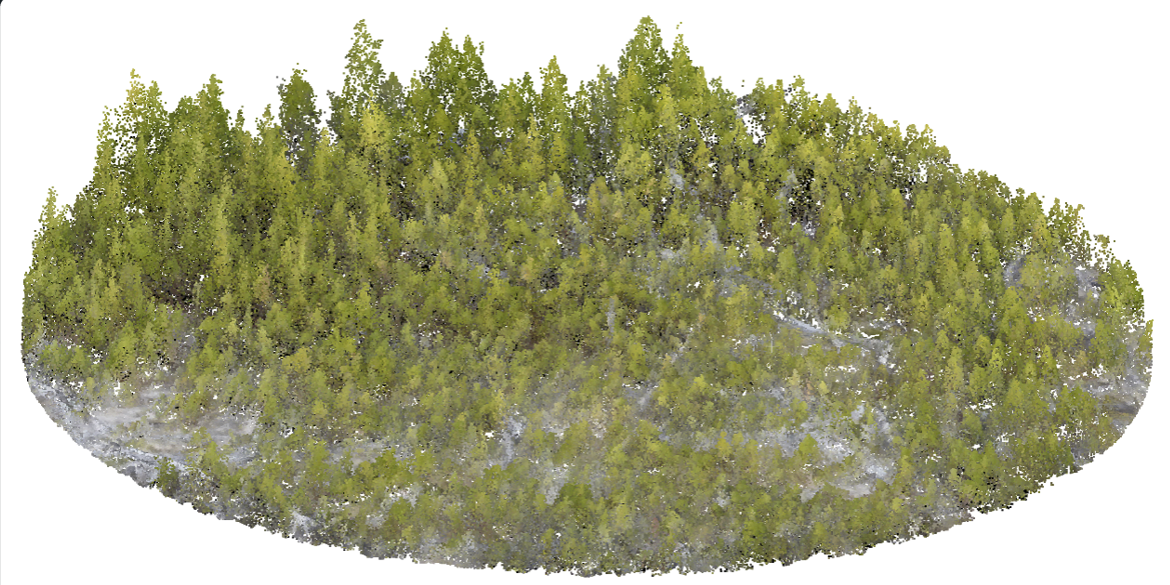
\includegraphics[width=5.3125in,height=\textheight]{images/clipboard-543746522.png}

}

\end{figure}

To gain a better understanding of how to use tree allometric models for
volume, taper, merchantable length/height, log volume, and biomass. If
you are comfortable working with R or python for this lab please feel
free to do so. This lab does not require using R for final computations.
To successfully run this lab in code format feel free to talk to your
TA. Instructions are given for the excel version.

\begin{center}\rule{0.5\linewidth}{0.5pt}\end{center}

\hypertarget{learning-objectives-4}{%
\section*{Learning Objectives}\label{learning-objectives-4}}
\addcontentsline{toc}{section}{Learning Objectives}

\markright{Learning Objectives}

\begin{itemize}
\tightlist
\item
  Use allometric equations to get merchantable volume, merchantable
  length and height, log-volum, and biomass.
\item
  Compare the results of different volume models.
\item
  Engage with scientific literature to find relevant models to calculate
  biomass and volume
\end{itemize}

\hypertarget{task-1---total-volume}{%
\section*{Task 1 - Total Volume}\label{task-1---total-volume}}
\addcontentsline{toc}{section}{Task 1 - Total Volume}

\markright{Task 1 - Total Volume}

\textbf{General Description}

\hypertarget{question-1-4}{%
\subsection*{Question 1}\label{question-1-4}}
\addcontentsline{toc}{subsection}{Question 1}

\begin{enumerate}
\def\labelenumi{\arabic{enumi}.}
\tightlist
\item
  Calculate \ul{the estimated total tree volume} for a hybrid spruce
  (Picea \emph{glauca} (Moench) Voss X P. e\emph{nglemannii} Parry ex
  Engelm.) tree growing in the ESSF near Smithers, BC with a DBH=80.0 cm
  and height= 35.0 m \ul{using the Kozak (2002) taper model}.
\item
  Use the EXCEL example provided modify necessary values for DBH,
  height, and betas (see the top of the sheet).
\item
  Once modified, get the total volume as well as a taper graph. Input
  both of these as your answer to question
\end{enumerate}

\hypertarget{question-2-.unnumbered-calculate-the-estimated-total-tree-volume-for-a-hybrid-spruce-picea-glauca-moench-voss-x-p.-englemannii-parry-ex-engelm.-tree-growing-in-the-essf-near-smithers-bc-with-a-dbh20.0-cm-and-and-12.0-m-in-height.-do-this-as-well-for-a-tree-of-100-cm-and-42.0-m-in-height.-in-your-answer-for-this-question-include-a-3-row-table-with-the-volumes-dbh-and-height-of-each-tree.}{%
\subsection{\texorpdfstring{Question 2 \{.unnumbered\} Calculate \ul{the
estimated total tree volume} for a hybrid spruce (Picea \emph{glauca}
(Moench) Voss X P. \emph{englemannii} Parry ex Engelm.) tree growing in
the ESSF near Smithers, BC with a DBH=20.0 cm and and 12.0 m in height.
Do this as well for a tree of 100 cm and 42.0 m in height. In your
answer for this question, include a 3 row table with the volumes, DBH,
and height of each
tree.}{Question 2 \{.unnumbered\} Calculate the estimated total tree volume for a hybrid spruce (Picea glauca (Moench) Voss X P. englemannii Parry ex Engelm.) tree growing in the ESSF near Smithers, BC with a DBH=20.0 cm and and 12.0 m in height. Do this as well for a tree of 100 cm and 42.0 m in height. In your answer for this question, include a 3 row table with the volumes, DBH, and height of each tree.}}\label{question-2-.unnumbered-calculate-the-estimated-total-tree-volume-for-a-hybrid-spruce-picea-glauca-moench-voss-x-p.-englemannii-parry-ex-engelm.-tree-growing-in-the-essf-near-smithers-bc-with-a-dbh20.0-cm-and-and-12.0-m-in-height.-do-this-as-well-for-a-tree-of-100-cm-and-42.0-m-in-height.-in-your-answer-for-this-question-include-a-3-row-table-with-the-volumes-dbh-and-height-of-each-tree.}}

\hypertarget{question-3-4}{%
\subsection*{Question 3}\label{question-3-4}}
\addcontentsline{toc}{subsection}{Question 3}

Compare the estimated taper shape for the original tree to the smaller
and larger trees in a short report. Why would this shape change for
different tree sizes? How does this ``help'' the tree? Give at least two
reasons why the shape changes as the tree size gets larger. Add in the
three graphs of tree shapes to your short report to support your
statements.

\hypertarget{task-2---merchantable-volume}{%
\section*{Task 2 - Merchantable
Volume}\label{task-2---merchantable-volume}}
\addcontentsline{toc}{section}{Task 2 - Merchantable Volume}

\markright{Task 2 - Merchantable Volume}

\hypertarget{question-4-4}{%
\subsection*{Question 4}\label{question-4-4}}
\addcontentsline{toc}{subsection}{Question 4}

Use the Kozak (2002) taper model again, but this time to calculate the
estimated merchantable volume for the large tree from a 0.3 m stump
height to a 10.0 cm top diameter inside bark. Some parts of the tree
will not be included in this merchantable volume and will have a zero
volume, namely the stump segment, and the parts of the tree above 10.0
cm top diameter inside bark. You will have to modify the section lengths
to obtain a 10.0 cm top diameter inside bark and then sections higher
than this will have a zero volume. What is the merchantable tree volume?
Again, keep four decimals only.

\hypertarget{question-5-4}{%
\subsection*{Question 5}\label{question-5-4}}
\addcontentsline{toc}{subsection}{Question 5}

Determine the estimated merchantable height (i.e., ground to
merchantable limit) and the estimated merchantable length (i.e., stump
to merchantable limit) of this tree. You will not be modifying your
Merchantable Volume worksheet for this; instead, use the worksheet to
get the answers (i.e.~when is the tree too small in width). The
merchantable length and merchantable height will be in m. By convention,
we keep one decimal place for tree heights and for merchantable lengths.
NOTE: We often keep two decimals for distances, and for log lengths,
however, and we keep one decimal place for DBH in cm.

\hypertarget{question-6-2}{%
\subsection*{Question 6}\label{question-6-2}}
\addcontentsline{toc}{subsection}{Question 6}

What is the merchantable volume over total volume proportion? If the
tree was larger, would this proportion be smaller or larger?

\hypertarget{question-7-2}{%
\subsection*{Question 7}\label{question-7-2}}
\addcontentsline{toc}{subsection}{Question 7}

How many logs of 2.5 m long could we get from this tree, within the
boundaries of the stump height and the minimum diameter inside bark of
10.0 cm? What could be done with the rest of the merchantable part of
the tree?

\hypertarget{question-8-bonus}{%
\subsection*{\texorpdfstring{\textbf{Question 8}
\emph{Bonus}}{Question 8 Bonus}}\label{question-8-bonus}}
\addcontentsline{toc}{subsection}{\textbf{Question 8} \emph{Bonus}}

What is the value of the first log (i.e., the largest one starting at
stump height) in CAD, assuming it is a high-quality log (i.e., no decay,
no knots, few growth rings per inch, and no defects)? HINT: You will
need to look up log prices online. You may also need the log grade given
the species, log size, and condition to estimate a likely log price.

\hypertarget{task-3---whole-tree-volume-models}{%
\section*{Task 3 - Whole Tree Volume
Models}\label{task-3---whole-tree-volume-models}}
\addcontentsline{toc}{section}{Task 3 - Whole Tree Volume Models}

\markright{Task 3 - Whole Tree Volume Models}

For the same tree large hybrid spruce as in Question 1 of Part I,
calculate the estimated total volume using the BC coefficients based on
Schumacher's model (Schumacher and Hall, 1933), but fitted using BC tree
data, and compare this to volume using Kozak's model.You will need to
use the Key Equations from Excercise 4 to calculate the volume using the
mature douglas fir coefficients. \#\#\# Question 9 \{.unnumbered\}
Compare this to the estimated total volume you calculated using Kozak's
taper model for this large hybrid spruce. NOTES: Since these were both
found using models, they are both estimated volumes. However, on one
hand, the volume models would be expected to be more precise for
estimating tree volume since they estimate this directly whereas the
volume using the taper model are calculated by first calculating the
estimated diameters inside bark up the stem. On the other hand, taper
models can be used for more than just estimated total volume (i.e.,
merchantable volume, log volumes, etc. as you did in Task 1 \& 2).

\hypertarget{task-4---engaging-with-the-literature}{%
\section{Task 4 - Engaging with the
literature}\label{task-4---engaging-with-the-literature}}

\hypertarget{question-10-3}{%
\subsection*{Question 10}\label{question-10-3}}
\addcontentsline{toc}{subsection}{Question 10}

\begin{enumerate}
\def\labelenumi{\arabic{enumi}.}
\tightlist
\item
  You used biomass models by Standish et al.~(1985) in Exercise 4 to
  find aboveground total biomass for trees in fixed-area plots. Find the
  following publication for tree biomass models of several species in
  Australia:
\end{enumerate}

\begin{tcolorbox}[enhanced jigsaw, colbacktitle=quarto-callout-tip-color!10!white, leftrule=.75mm, left=2mm, opacitybacktitle=0.6, breakable, colframe=quarto-callout-tip-color-frame, arc=.35mm, bottomtitle=1mm, rightrule=.15mm, title={Search the Literature}, toptitle=1mm, titlerule=0mm, opacityback=0, coltitle=black, colback=white, bottomrule=.15mm, toprule=.15mm]

Bi H, S Murphy, L Volkova, C Weston, T Fairman, Y Li, R Law, J Norris, X
Lei, G. 2015. Additive biomass equations based on complete weighing of
sample trees for open eucalypt forest species in south-eastern
Australia. Forest Ecology and Management Volume 349, pages 106 to 121.
https://doi.org/10.1016/j.foreco.2015.03.007

\end{tcolorbox}

Then, estimate the aboveground biomass (kg) for a E. regnans that is
120.0 cm DBH (Note: Measured at 1.37 m above ground in Australia) and
51.0 m in height. For this, use Eq. 8 that uses DBH only (labelled as D,
cm) or Eq. 10 that uses D2H,(DBH (cm) squared time height (m)) from the
paper. The parameter estimates for each of these models and that species
are found in Table 2. You will need to calculate the total stem biomass
and the crown biomass first, and add them together to get total tree
(aboveground) biomass, as shown in Eq. 8 or 10, to get aboveground
biomass. :::\{.callout-note\} NOTE: You might want to input these DBH
and height measures into Standish et al.~(1985) biomass model for mature
Coastal Douglas-fir that you already used in Exercise 4 to estimate the
kg and use that as a rough guide as to what the estimated biomass might
be for this E. regnans tree using the Bi et al.~(2015) models. :::

\hypertarget{question-11-bonus}{%
\subsection*{\texorpdfstring{\textbf{Question 11}
\emph{Bonus}}{Question 11 Bonus}}\label{question-11-bonus}}
\addcontentsline{toc}{subsection}{\textbf{Question 11} \emph{Bonus}}

Find a publication with a tree biomass model for white spruce (Picea
glauca (Moench) Voss growing in Ontario, Canada. Give the full citation
for this publication. (See Question 10 for an example of a full
citation).

\begin{center}\rule{0.5\linewidth}{0.5pt}\end{center}

\hypertarget{lab-questions-deliverables-4}{%
\section*{Lab Questions \&
Deliverables}\label{lab-questions-deliverables-4}}
\addcontentsline{toc}{section}{Lab Questions \& Deliverables}

\markright{Lab Questions \& Deliverables}

\begin{itemize}
\tightlist
\item[$\square$]
  Complete answers for all 11 questions in the lab \emph{including
  graphs and tables with captions and proper units}
\end{itemize}

\hypertarget{summary-4}{%
\section*{Summary}\label{summary-4}}
\addcontentsline{toc}{section}{Summary}

\markright{Summary}

In this lab, we used a taper model to estimate total tree volume,
merchantable volume, merchantable height, and merchantable length. We
also compared the results of different volume models and engaged with
scientific literature to find relevant models to calculate biomass and
volume.

\bookmarksetup{startatroot}

\hypertarget{vdyp-tipsy-for-forecasting-inventory-records}{%
\chapter{06 - VDYP \& TIPSY for Forecasting Inventory
Records}\label{vdyp-tipsy-for-forecasting-inventory-records}}

\hypertarget{lab-overview-5}{%
\section*{Lab Overview}\label{lab-overview-5}}
\addcontentsline{toc}{section}{Lab Overview}

\markright{Lab Overview}

For timber supply (and other forest-level analyses), forecasts of each
stand (or aggregates of similar stands) are needed to evaluate different
management scenarios. For these analyses, yield tables for each stand
type and management regime are needed to make these forecasts. In BC,
VDYP is used for ``unmanaged'' stands and TIPSY is used for ``managed''
stands. There are other models (e.g., PrognosisBC) also available for
use by BC forest professionals. :::\{.callout-note collapse=`true'\}
\#\# Growth \& Yield Models in BC

\textbf{TIPSY}

\begin{itemize}
\item
  For managed stands
\item
  Used in Timber Supply Analysis for managed stands (i.e., post harvest)
\item
  Can also be used for ``silvicultural gaming''
\item
  Prorates pure species stand yields to get mixed species stand yields
  (as does VDYP)
\item
  Can add silvicultural treatments
\item
  Look up forecasts from a database using the input variables you supply

  \begin{itemize}
  \tightlist
  \item
    Where did this database come from? Run TASS -\textgreater{} get
    yield tables and other things -\textgreater{} add to TIPSY's
    database -\textgreater{} now ready to use in TIPSY - Where is TASS
    from?
  \item
    About 50 years of research using primarily data from experimental
    installations (not representative of the landbase)
  \end{itemize}
\item
  Limited options -- More in TASS (not yet available to everyone)
\item
  When you run TIPSY, you get access to TIPSY help -- very useful!! Lots
  of info there.
\item
  \textbf{Inputs needed} (* indicates these are optional)

  \begin{itemize}
  \tightlist
  \item
    Species composition
  \item
    OAFs: The TASS and TIPSY yields will be too high because they assume
    no forest gaps, and low rates of pathogen/insect attacks.
  \end{itemize}
\item
  \textbf{Outputs obtained}

  \begin{itemize}
  \tightlist
  \item
    Volume per ha over age
  \item
    MAI (m3/ha/year) over age
  \end{itemize}

  \textbf{VDYP}
\item
  For ``naturally-regenerated'' stands (so-called ``unmanaged'' stands)
\item
  Used in Timber Supply Analysis for unmanaged stands (i.e., naturally
  regenerated)
\item
  Data used is more representative of the land base (not simple random
  sampling, but more representative)
\item
  Prorates yields of pure species stands to get mixed species (as does
  TASS)
\item
  \textbf{Inputs needed}

  \begin{itemize}
  \tightlist
  \item
    Species composition
  \item
    BEC zone
  \item
    Site productivity: Site index OR site height + age (SI calculated)
  \item
    Density
  \end{itemize}
\item
  \textbf{Outputs obtained}

  \begin{itemize}
  \item
    Volume per ha over age
  \item
    MAI (m3/ha/year) over age

    \textbf{TASS}
  \end{itemize}
\item
  Tree-level distance dependent model developed for managed stands
\item
  Is the ``engine'' behind TIPSY database
\item
  New version coming out soon (beta-testing right now) that will be
  available to more users
\item
  Grows each tree crown and then the stem from this crown growth
\item
  Competition depends on overlap of crowns
\item
  50 years of research

  \textbf{SORTIEBC}
\item
  Tree-level distance dependent model that is considered a ``hybrid''
  model since competition is based on light interception by crowns
\item
  Limited support by BC MFLNRO right now
\item
  SORTIE was originally developed by Canham in the USA.

  \textbf{PROGNOSIS BC}
\item
  Tree-level, distance independent model for mixed-species stands
  (managed or natural)
\item
  Is the GY model behind the FVS system (most locations, not all) that
  has been adopted for use throughout the USA.
\item
  Not supported by BC MFLNRO right now (``moth-balled'')
\item
  Original Prognosis model was developed by Stage (1973 publication)

  \textbf{Others}
\item
  Forsyte, Forsee, Fortoon: Developed by Kimmins, professor emeritus at
  UBC. A hybrid model. Zelig: GAP model MGM: Developed for mixed species
  stands at the University of Alberta by Titus
\item
  \emph{every province has its own collection (e.g.~PROGNOSIS Ontario,
  GYPSY (Alberta), etc.)} :::
\end{itemize}

To become familiar with how VDYP and TIPSY can be used to forecast the
growth and yield of stands, you will forecast three polygons from MKRF.
You will use the VRI forest inventory, layer 1 attributes, as inputs to
VDYP. This links the VDYP model to forest inventory information, which
is what happens for ``unmanaged'' stands in timber supply analyses. You
will then simulate harvests of these stands and forecast future growth
and yield post-harvest using TIPSY.

\begin{center}\rule{0.5\linewidth}{0.5pt}\end{center}

\hypertarget{learning-objectives-5}{%
\section*{Learning Objectives}\label{learning-objectives-5}}
\addcontentsline{toc}{section}{Learning Objectives}

\markright{Learning Objectives}

\begin{itemize}
\item
  Understand the application of TIPSY and VDYP on the landbase
\item
  Utilize TIPSY and VDYP to better understand forecasting for management
  decisions.
\end{itemize}

\begin{center}\rule{0.5\linewidth}{0.5pt}\end{center}

\hypertarget{task-1-vdyp-stand-level-yield-forecasts-using-vri-as-inputs}{%
\section*{Task 1 VDYP: Stand-level Yield Forecasts using VRI as
Inputs}\label{task-1-vdyp-stand-level-yield-forecasts-using-vri-as-inputs}}
\addcontentsline{toc}{section}{Task 1 VDYP: Stand-level Yield Forecasts
using VRI as Inputs}

\markright{Task 1 VDYP: Stand-level Yield Forecasts using VRI as Inputs}

You looked at the 2014 VRI forest cover for MKRF in FRST 556, Ex.1 and
2. Using these data, all stands where western redcedar (\emph{Thuja
plicata}) was species with the largest percent were selected using QGIS.
The attributes were exported as a .csv file, which was sorted,
attributes were trimmed (i.e., some attributes were removed), and then
the results were saved as CW dominated polygons trimmed.xlsx. Three of
these stands in the northwestern part of MKRF were selected as stands of
interest (CW dominated three polygons trimmed.xlsx). A few of the
attributes of these polygons are shown in Table~\ref{tbl-polys}, and an
image of the location of these stands is shown in Figure 1

\hypertarget{tbl-polys}{}
\begin{longtable}[]{@{}
  >{\raggedright\arraybackslash}p{(\columnwidth - 10\tabcolsep) * \real{0.0909}}
  >{\raggedright\arraybackslash}p{(\columnwidth - 10\tabcolsep) * \real{0.1558}}
  >{\raggedright\arraybackslash}p{(\columnwidth - 10\tabcolsep) * \real{0.1558}}
  >{\raggedright\arraybackslash}p{(\columnwidth - 10\tabcolsep) * \real{0.1558}}
  >{\raggedright\arraybackslash}p{(\columnwidth - 10\tabcolsep) * \real{0.2078}}
  >{\raggedright\arraybackslash}p{(\columnwidth - 10\tabcolsep) * \real{0.2338}}@{}}
\caption{\label{tbl-polys}Table 1. Three polygons selected from the
western redcedar dominated stands of MKRF (Data Source: VRI 2014 forest
cover map, layer 1).}\tabularnewline
\toprule\noalign{}
\begin{minipage}[b]{\linewidth}\raggedright
LY\_ID
\end{minipage} & \begin{minipage}[b]{\linewidth}\raggedright
LBL\_SPECIS
\end{minipage} & \begin{minipage}[b]{\linewidth}\raggedright
EST\_SI\_SPC
\end{minipage} & \begin{minipage}[b]{\linewidth}\raggedright
EST\_SI (m)
\end{minipage} & \begin{minipage}[b]{\linewidth}\raggedright
CR\_CLOSURE (\%)
\end{minipage} & \begin{minipage}[b]{\linewidth}\raggedright
Shape\_Ar (in ha)
\end{minipage} \\
\midrule\noalign{}
\endfirsthead
\toprule\noalign{}
\begin{minipage}[b]{\linewidth}\raggedright
LY\_ID
\end{minipage} & \begin{minipage}[b]{\linewidth}\raggedright
LBL\_SPECIS
\end{minipage} & \begin{minipage}[b]{\linewidth}\raggedright
EST\_SI\_SPC
\end{minipage} & \begin{minipage}[b]{\linewidth}\raggedright
EST\_SI (m)
\end{minipage} & \begin{minipage}[b]{\linewidth}\raggedright
CR\_CLOSURE (\%)
\end{minipage} & \begin{minipage}[b]{\linewidth}\raggedright
Shape\_Ar (in ha)
\end{minipage} \\
\midrule\noalign{}
\endhead
\bottomrule\noalign{}
\endlastfoot
611 & CwHw(Fd) & CW & 20 & 65 & 11.1 \\
621 & CwHw(Fd) & CW & 21 & 65 & 2.1 \\
622 & CwHw(Fd) & CW & 18 & 70 & 7.1 \\
\end{longtable}

\begin{tcolorbox}[enhanced jigsaw, colbacktitle=quarto-callout-note-color!10!white, leftrule=.75mm, left=2mm, opacitybacktitle=0.6, breakable, colframe=quarto-callout-note-color-frame, arc=.35mm, bottomtitle=1mm, rightrule=.15mm, title=\textcolor{quarto-callout-note-color}{\faInfo}\hspace{0.5em}{Table Notes}, toptitle=1mm, titlerule=0mm, opacityback=0, coltitle=black, colback=white, bottomrule=.15mm, toprule=.15mm]

• POLY\_ID is the ID for the polygon: • LBL\_SPECIS shows the species
from the highest to lowest percent (species in brackets have very low
percentages) • EXT\_SI\_SPC is the species used for the site index
reported; EST\_SI is the site index for the stand in m; • CR\_CLOSURE is
the percent of the ground covered by trees; and • Shape\_Area is
reported in m2 by QGIS (and in ARCGIS software), but these have been
converted to ha (This may be less than POLY\_AREA in the VRI data, since
the polygon may extend outside of the MKRF boundary).

\end{tcolorbox}

\begin{figure}

{\centering 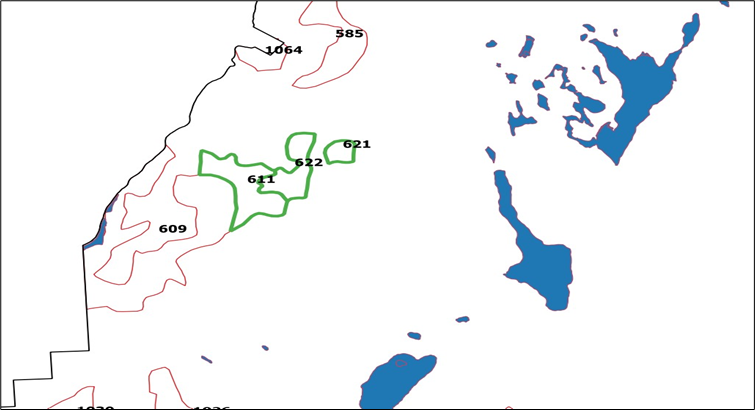
\includegraphics{images/clipboard-1804548772.png}

}

\caption{Figure 1. Map of three selected (in green) western redcedar
dominated polygons of MKRF. (Data Source: VRI 2014 forest cover map,
layer 1).}

\end{figure}

In the CW dominated three polygons \textbf{trimmed.xlsx} file, you will
also find the species percentages for these three selected polygons, and
other attributes that you may need as inputs to VDYP to forecast this
stand. Using VDYP, forecast these three stands from 0 to 250 years total
age at 10-year intervals. You will get a yield a yield trajectory for
each attribute in each of three stands (i.e., total volume per ha,
merchantable volume per ha, stems per ha, etc. over time).

\begin{enumerate}
\def\labelenumi{\arabic{enumi}.}
\item
  To get you started, first do the example stand in the Quick Intro to
  VDYP7.pdf (or .docx) file to get the yield trajectory, export these to
  EXCEL, trim off any labels, and then graphs the trajectories.
\item
  Use similar steps to get forecasts for each of these three stands, and
  export growth and yield table to an EXCEL file. Include merchantable
  volume (12.5 + cm DBH) in your outputs, as well as the MAI's for total
  and merchantable volume. (See POLYGON1 2020 VDYP trimmed.xlsx as an
  example of VDYP outputs for a stand).
\item
  Using these growth and yield outputs, answer the questions posed and
  put these answers in your submission
\end{enumerate}

\hypertarget{question-1-vdyp-questions}{%
\subsection{Question 1 (VDYP
Questions)}\label{question-1-vdyp-questions}}

\begin{enumerate}
\def\labelenumi{\arabic{enumi}.}
\tightlist
\item
  Graph the total volume per ha (m\textsuperscript{3}/ha) over total age
  (years) for each stand.~ Which stand appears to be the most
  productive? Explain your answer.~
\item
  Graph the total volume mean annual increment (MAI or m.a.i.,
  m\textsuperscript{3}/ha/year) over total age for each of these three
  stands.~~ What is the biological rotation age for each stand?
\end{enumerate}

\begin{figure}

{\centering 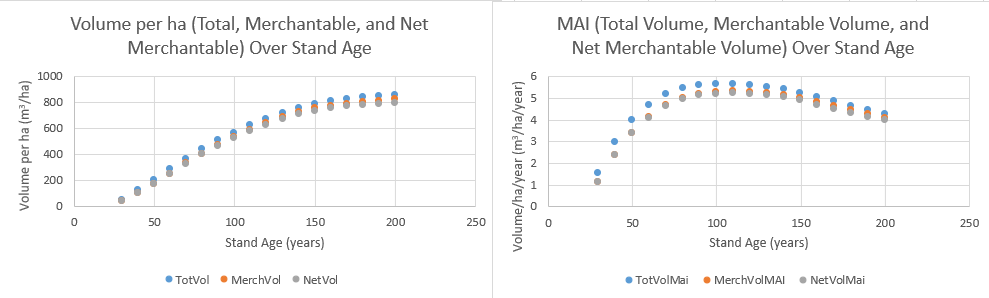
\includegraphics{images/clipboard-1872295870.png}

}

\caption{Figure 2. Example of the total volume per ha and MAI for three
selected stands.}

\end{figure}

\begin{enumerate}
\def\labelenumi{\arabic{enumi}.}
\setcounter{enumi}{2}
\tightlist
\item
  Repeat \#2, but this time use the merchantable volume per ha (i.e.,
  all trees 12.5 cm + DBH).~~ Are the biological rotation ages different
  than using the total volume per ha?
\item
  For each stand, what is the merchantable volume per ha (12.5 cm + DBH)
  at the biological rotation age (i.e., at the maximum m.a.i. for this
  volume)?~ What is the average tree size in terms of average height
  (here Lorey's height) and average DBH (here Quadratic Mean DBH)?
\item
  For each stand, what is current, estimated merchantable volume (12.5
  cm + DBH) for the entire stand? HINT: First, determine the stand age
  as of 2014 using the VRI polygon attributes, and adjust this age to
  current year (2024) Then, look up the merchantable volume per ha (12.5
  cm+ DBH) for that stand age. Finally, determine the current
  merchantable volume for the entire stand.
\item
  Based on the information you now have, would you recommend that any of
  these stands be harvested in the next 10 years or not? Explain your
  answer.
\end{enumerate}

\begin{center}\rule{0.5\linewidth}{0.5pt}\end{center}

\hypertarget{task-2---forecasting-using-tipsy}{%
\section{Task 2 - Forecasting Using
TIPSY}\label{task-2---forecasting-using-tipsy}}

If these stands were harvested, we would need to forecast the stands
again post-harvest. This is less complicated if stands were clearcut
(i.e., called a \emph{regeneration cut} or \emph{clearfelling} in some
places in the world), than if the stands were partially harvested.~ We
will assume that each of these stands was clearcut and you want to
project the stands after harvest.~ Following harvest:

\begin{itemize}
\item
  We could assume that the stands will naturally follow the \ul{same
  trajectory} as prior to harvest, meaning that they will start again at
  total age = 0 and follow the VDYP trajectories you created in Part I.~
\item
  Alternatively, we could plant the pre-harvest dominant species or a
  different species, control the planting density, and forecast each
  stand using this management regime. We would then forecast the stand
  using TIPSY.
\end{itemize}

Here, we will assume that \ul{\textbf{you will plant 1600 stems/ha of
Coastal Douglas-fir following harvest}}. For each stand, show the
\ul{\textbf{forecast trajectories from 0 to 150 years by 10-year
intervals},} as you did previously for the existing stand using VDYP,
but this time using TIPSY for ``managed'' stands.~ You will need to use
some of the VRI information from the old stand that was there prior to
harvest in doing the trajectory (e.g., Site Index).~ Before you do these
stand forecasts, \ul{\textbf{do the forecast for the example stand}} in
the \textbf{Quick Guide to Using TIPSY 4.4.docx (}or pdf).

\hypertarget{question-2-tipsy-questions}{%
\subsection{Question 2 (TIPSY
Questions)}\label{question-2-tipsy-questions}}

Using EXCEL and the outputs from your VDYP and TIPSY forecasts:

\begin{enumerate}
\def\labelenumi{\arabic{enumi}.}
\tightlist
\item
  For the post-harvest plan, 1600 stems/ha was used. What is the spacing
  between the trees (m) assuming square spacing? Show your calculations.
\item
  Coastal Douglas-fir (FD) was used as the species to be planted
  post-harvest, whereas CW was the main species in the original stands
  at the time of the VRI inventory (Reference year: 1999). Since the
  Site Index was for CW not for FD, is the TIPSY forecast reliable?
  Explain briefly, considering the ecology of these three species in
  CWH.
\item
  Graph the total volume per ha (m\textsuperscript{3}/ha) over total age
  (years) for the post-harvest TIPSY forecast versus the VDYP forecast
  for each of these stands (NOTE: The TIPSY forecast will be for 0 to
  150 years only).~ Compare these trajectories, and explain why they are
  different using principles of stand and tree growth for the existing
  stand versus the post-harvest planted stand.
\item
  Is the cost of planting justified? Briefly discuss under what
  circumstances this cost would be justified for these three stands.
\end{enumerate}

\begin{center}\rule{0.5\linewidth}{0.5pt}\end{center}

\hypertarget{lab-questions-deliverables-5}{%
\section*{Lab Questions \&
Deliverables}\label{lab-questions-deliverables-5}}
\addcontentsline{toc}{section}{Lab Questions \& Deliverables}

\markright{Lab Questions \& Deliverables}

\begin{itemize}
\tightlist
\item[$\square$]
  Complete answers VDYP Questions
\item[$\square$]
  Complete answers for TIPSY questions
\item[$\square$]
  \emph{all graphs and tables have captions and proper units}
\end{itemize}

\hypertarget{summary-5}{%
\section*{Summary}\label{summary-5}}
\addcontentsline{toc}{section}{Summary}

\markright{Summary}

\bookmarksetup{startatroot}

\hypertarget{data-description-for-frst-556-course-data}{%
\chapter{Data Description for FRST 556 course
data}\label{data-description-for-frst-556-course-data}}

\hypertarget{sec-data}{%
\section{Course Data}\label{sec-data}}

Written by

Sarah Smith-Tripp

FRST 556 is mostly concentrated on Malcom Knapp Research Forest (MKRF)
located outside of Maple Ridge, British Columbia. The research forest
maintains an extensive GIS database available to researchers and
students alike. We have included the necessary files in the material
posted on the UBC canvas page. Casual users can access the data here:
\href{https://www.mkrf.forestry.ubc.ca/education/gis/}{Access MKRF Data}

\hypertarget{data-incorporated-in-course-material}{%
\section{Data Incorporated in Course
Material}\label{data-incorporated-in-course-material}}

The original GIS material available from MKRF have been converted from
the ESRI geodatabase format into a series of geopackages. In the folder,
the first letter describes the datatype. These are described in the
table below in addition to the data included

\begin{longtable}[]{@{}
  >{\raggedright\arraybackslash}p{(\columnwidth - 4\tabcolsep) * \real{0.0794}}
  >{\raggedright\arraybackslash}p{(\columnwidth - 4\tabcolsep) * \real{0.0529}}
  >{\raggedright\arraybackslash}p{(\columnwidth - 4\tabcolsep) * \real{0.8624}}@{}}
\caption{Description of Files included in the
`Data\_Folder'}\tabularnewline
\toprule\noalign{}
\begin{minipage}[b]{\linewidth}\raggedright
Start Letter
\end{minipage} & \begin{minipage}[b]{\linewidth}\raggedright
Type
\end{minipage} & \begin{minipage}[b]{\linewidth}\raggedright
Description
\end{minipage} \\
\midrule\noalign{}
\endfirsthead
\toprule\noalign{}
\begin{minipage}[b]{\linewidth}\raggedright
Start Letter
\end{minipage} & \begin{minipage}[b]{\linewidth}\raggedright
Type
\end{minipage} & \begin{minipage}[b]{\linewidth}\raggedright
Description
\end{minipage} \\
\midrule\noalign{}
\endhead
\bottomrule\noalign{}
\endlastfoot
I & Image & I\_2006\_MKRF\_RGB.ecw - 2006 aerial RGB image

I\_2008\_MKRF\_RGB.tif - 2008 mosaiced aerial RGB image

\includegraphics{.pdf}I\_2019\_LandsatBAP\_MKRF-01.tif - 2019
`\href{https://code.earthengine.google.com/e27240a92ecf64bbadf8a082b91c711c?hideCode=true}{Best
Available Pixel}' composite

I\_Lake\_Mask\_MKRF.tif - Binary mask of Lakes within MKRF Boundaer \\
L & Line & L\_contours\_1m.gpkg - 1 m elevation contours

L\_contours\_5m.gpkg - 5 m elevation contours

L\_hydroline.gkpg - Location of hydroline crossing MKRF

L\_roads\_y2010.gpkg - Location of roads (as of 2010)

L\_streams\_major.gkpg - Major streams

L\_streams.gkpg - all streams

L\_trails.gkpg - Location of trails within MKRF \\
P & Polygon & P\_BC\_Biogeoclimatic.gpkg - Biogeoclimatic areas of MRKF

P\_BC\_VRI\_2014.gpkg - 2014 VRI based on 1996 aerial imagery and then
updated (i.e.~projected) to 2014

P\_Boundary\_MKRF.gpkg - MKRF boundary

P\_BoundaryWoodlot.gpkg - Boundary for woodlot adjacent to MKRF also
managed by MKRF staff

P\_Buildings.gpkg - Location of structures for Loon Lake Retreat Center

P\_ForestCover\_1989.gpkg - Photo- interpretation of forest cover from
BC sterography

P\_ForestCover\_1999.gpkg - Updated version of the 1989 assessment based
on known locations of human and natural disturbances

P\_ForestCover\_2008.gpkg - Updated version of 1989 and 1999 assessment
based on known location of human and natural disturbances

P\_ForestDevelopmentPlan\_2019.gpkg - Location of forest development
plans as per 2019

P\_lakes.gpgk - Polygon of lakes in MKRF

P\_proposedharvest\_y2020.gpkg - Location of proposed harvests as of
2020

P\_proposedharvest\_y2023.gpkg - Location of proposed harvests as of
2023

P\_ReserveAreas.gpkg - Location of reserves where generally no harvest
occur (except for safety issues) \\
Pts & Points & Pts\_SelectiveSampling\_2016.gpkg - Locations of
selective sampling for 2016

Pts\_SystematiceSampling\_1995.gpkg - Locations of the systematic
sampling areas \\
\end{longtable}

\bookmarksetup{startatroot}

\hypertarget{sec-fieldcodes}{%
\chapter{Field Code Descriptions for ``Forest Cover''
Layers}\label{sec-fieldcodes}}

\begin{longtable}[]{@{}
  >{\raggedright\arraybackslash}p{(\columnwidth - 4\tabcolsep) * \real{0.0604}}
  >{\raggedright\arraybackslash}p{(\columnwidth - 4\tabcolsep) * \real{0.0687}}
  >{\raggedright\arraybackslash}p{(\columnwidth - 4\tabcolsep) * \real{0.8709}}@{}}
\toprule\noalign{}
\begin{minipage}[b]{\linewidth}\raggedright
Type
\end{minipage} & \begin{minipage}[b]{\linewidth}\raggedright
Field
\end{minipage} & \begin{minipage}[b]{\linewidth}\raggedright
Description
\end{minipage} \\
\midrule\noalign{}
\endhead
\bottomrule\noalign{}
\endlastfoot
Description & SHAPE & Internally ArcView \\
Description & Fc99\# & Internally Arc/INFO \\
Description & Fc99-id & Internally Arc/INFO \\
Description & Poly\# & Internally Arc/INFO \\
Description & Subclass & Internally Arc/INFO \\
Description & Subclass\# & Internally Arc/INFO \\
Description & Rings\_ok & Internally Arc/INFO \\
Description & Rings\_nok & Internally Arc/INFO \\
Description & ID & Polygon ID -- unique for every polygon in the map \\
Description & AREA & Polygon area \\
Description & PERIMETER & Polygon perimeter \\
Description & MAPNO & Map number (1, 2 or 3) \\
Description & UID & Unit ID -- Combination of map sheet number and
polygon ID \\
Description & UID2 & Unit ID Specification -- range from ``a'' to ``z''
and is due to the process of splitting the initial polygons by the
partial cuttings \\
Description & NAME & Ex. 97A80\_01 97-Date of treatment, A80-name of
road, \_01- \# of cutblock along road \\
Description & TREATMENT & Silvicultural Treatment (Clearcut or
Thinning) \\
Description & LAYER & Horizontal stratum or layer: 1 - most important, 2
- next most important layer \\
Description & RANK & Order of importance of each layer in a
multi-layered stand \\
Description & NFD & Non-forest descriptor- \textbf{C} -- cultivated-
\textbf{LK} -- lake- \textbf{NCBR} -- non-commercial brush-
\textbf{NPBR} -- non-productive brush- \textbf{NP} -- non-productive-
\textbf{NSR} -- non-sufficiently restocked- \textbf{RIV} -- river-
\textbf{SW} --- \textbf{TS} -- mine tailing prevent growth- \textbf{U} -
urban \\
Description & DCLASS & Data collection class: 0 - photo interpretation,
1- air call, 8 - ground observation \\
Description & DSOURCE & Data collection source: 0 - no qualification, 1
- Ionut Aron, 2 - MRKF staff \\
Description & DATE\_IN & Data of the initial forest inventory
(YYMMDD) \\
Description & DATE\_PROJ & Date for any projected fields (YYMMDD) \\
Photo interpretation & SPCS1\ldots{} SPCS6 & Species from the most
prevalent (\textbf{SPSC1})- \textbf{AC} -- Balsam poplar- \textbf{H} --
Western hemlock- \textbf{F} -- Douglas-fir- \textbf{BG} -- Grand fir-
\textbf{D} -- Red alder- \textbf{C} -- Western redcedar- \textbf{L} --
Larch- \textbf{MB} -- Broadleaf maple- \textbf{CY} -- Yellow cedar-
\textbf{PL} -- Lodgepole pine- \textbf{PW} -- Western white pine \\
Photo interpretation & PCT1 \ldots{} PCT6 & Percentages for
\textbf{SPCS1} -- \textbf{SPCS6} \\
Photo interpretation & AGECL\_IN & Initial age class at the time of the
forest inventory- \textbf{1} - \textless20 years- \textbf{2} -- 21-40
years- \textbf{3} -- 41-60 years- \textbf{4} -- 61-80 years- \textbf{5}
-- 81-100 years- \textbf{6} -- 101-120 years- \textbf{7} -- 121-140
years- \textbf{8} -- 141-250 years- \textbf{9} - \textgreater{} 250
years \\
Photo interpretation & HTCL\_IN & Initial height class at the time of
the forest inventory- \textbf{1} - \textless{} 10.4 m- \textbf{2} --
10.5-19.4 m- \textbf{3} -- 19.5-28.4 m- \textbf{4} -- 28.5-37.4 m-
\textbf{5} -- 37.5-46.4 m- \textbf{6} -- 46.5-55.4 m- \textbf{7} --
55.5-64.4 m- \textbf{8} - \textgreater64.5 m \\
Photo interpretation & SITE\_IN & Site index class- \textbf{L} -- low-
\textbf{P} -- poor- \textbf{M} -- medium- \textbf{G} -- good \\
Photo interpretation & CRNCLCL & Crown closure class- \textbf{0} --
0-5\%- \textbf{1} -- 6-15\%- \textbf{2} -- 16-25\%- \textbf{3} --
26-35\%- \textbf{4} -- 36-45\%- \textbf{5} -- 46-55\%- \textbf{6} --
56-65\%- \textbf{7} -- 66-75\%- \textbf{8} -- 76-85\%- \textbf{9} --
86-95\%- \textbf{10} -- 96-100\% \\
Photo interpretation & BASICL & Basic Class -- the class or type of
non-productive areas- \textbf{0} -- Forest Cover- \textbf{3} -- Rock-
\textbf{4} -- This code does not appear in the Ministry of Forests'
documentation- \textbf{11} -- Non-productive brush- \textbf{12} --
Non-productive- \textbf{15} -- Lake- \textbf{25} -- River- \textbf{35}
-- Wwamp (muskeg)- \textbf{42} -- Clearing- \textbf{54} -- Urban \\
Photo interpretation & EPA & Environmentally sensitive areas-
\textbf{ER} -- High recreation- \textbf{RW} -- Recreation and wildlife-
\textbf{W} -- wildlife- \textbf{S} -- unstable \\
Derived Values & AGE\_PLANTE & Age of trees when planted \\
Derived Values & HEIGHT\_IN & Initial average height (m) \\
Derived Values & AGE\_IN & Initial stand age \\
Derived Values & SITEINDX & VDYP site index \\
Derived Values & VOL12\_5 & Average stand volume above 12.5 cm diameter
limit \\
Derived Values & VOL7\_5 & Average stand volume above 7.5 cm diameter
limit \\
Derived Values & DIAM12\_5 & Average stand diameter above 12.5 cm
diameter limit \\
Derived Values & DIAM7\_5 & Average stand diameter above 7.5 cm diameter
limit \\
Derived Values & CRNCLOS & Crown closure (\%) \\
Derived Values & DENSITY & Density (stems per hectare \\
Derived Values & REFYR & Reference year for update \\
Derived Values & AGE\_PROJ & Projected age -- range from 0 to 500
years \\
Derived Values & HEIGHT\_PRO & Projected height (m) -- range from 0 to
50 m \\
Derived Values & AGECL\_PROJ & Projected age class (same as Initial age
class coding) -- range from 1 to 9 \\
Derived Values & HTCL\_PROJ & Projected height class (same as Initial
height class coding) -- range from 1 to 8 \\
Derived Values & DATE\_EST & Date forest established calculated by
subtracting the mean age of the leading species of the stand or plot
from the calendar year that the measurement or estimate was made \\
Ground Data & DBH\_LIM & Diameter at Breast Height Limit -- minimum
diameter at breast height to which trees are to be recorded or measured
(all records have value of 22.5 cm) \\
Ground Data & BAGE & Age at breast height -- the number of annual rings
counted at 1.30 m height \\
Ground Data & BAGECORR & Breast age corrected to total age \\
Ground Data & TOPHT & Top Height -- average height of 100 trees of
largest diameter per hectare \\
Ground Data & GSPCS1 \ldots{} GSPCS3 & Same as \textbf{SPCS1} \ldots{}
\textbf{SPCS6} but data from ground observations \\
Ground Data & GPCT1 \ldots{} GPCT3 & Same as \textbf{PCT1} \ldots{}
\textbf{PCT6} but data from ground observations \\
Ground Data & BA\_HA\_SP1 \ldots BA\_HA\_SP3 & Basal area per hectare
for \textbf{SPCS1} \ldots{} \textbf{SPCS6} \\
Ground Data & SITE\_H\_SP1 \ldots{} SITE\_H\_SP3 & The height for the
site tree per species \\
\end{longtable}


\backmatter

\end{document}
